\documentclass[10pt,a4paper]{article}
\usepackage[margin=22mm]{geometry}
\usepackage{amsmath,amssymb}
\usepackage{booktabs}
\usepackage{longtable}
\usepackage{graphicx}
\usepackage{array}
\usepackage{enumitem}
\usepackage[table]{xcolor}
\usepackage[colorlinks=true,linkcolor=blue!50!black,urlcolor=blue!50!black]{hyperref}
\usepackage{microtype}
\usepackage{caption}
\usepackage{listings}
\lstset{basicstyle=\ttfamily\scriptsize, breaklines=true, breakatwhitespace=false,
  columns=fullflexible, keepspaces=true, frame=single, framesep=3pt, rulecolor=\color{black!25},
  xleftmargin=2pt, aboveskip=6pt, belowskip=6pt, showstringspaces=false, literate={\-}{{-}}1}

\graphicspath{{../}}
\newcommand{\fn}[1]{\nolinkurl{#1}}
\urlstyle{tt}
\makeatletter\def\UrlBreaks{\do\/\do\_\do\-\do\.\do\+\do\=\do\:}\makeatother
\setcounter{tocdepth}{2}
\newcommand{\NR}{\emph{not recorded}}
\setlength{\tabcolsep}{4pt}
\renewcommand{\arraystretch}{1.12}
\captionsetup{font=small}

\title{\bf Deployable Kirigami on Arbitrary Planar Graphs\\[2mm]
\large Internal run notebook --- autonomous ideation-to-demo run}
\author{Chronicler (Opus 5), for the Fable 5.1 orchestrator}
\date{Compiled 2026-09-04 from the repository at\\ \fn{/Users/emredayangac/Documents/kirigami-experiments}}

\begin{document}
\maketitle

\begin{abstract}
\noindent
This is an internal laboratory notebook, not a paper. It records, exhaustively and with file
citations, what the autonomous research run on deployable kirigami has done between
2026-09-03 and 2026-09-04: the two base papers and the errata found in them, three literature
screens, a from-scratch C\texttt{++} reimplementation of the 2026 pipeline and its parity against the
authors' own code, four personas' ideation and a hostile ranking, seven theorem families with
five rounds of adversarial checking, ten kill experiments, and a fabrication export path.
Every number below is traceable to a named file. Where a quantity is not on disk, the notebook
says \NR{} rather than supplying one. Two of the six deliverables of MISSION \S1
(\fn{IDEA.md} and \fn{REPORT.md}) do not yet exist; \S10 states exactly what is missing.
\end{abstract}

\tableofcontents
\newpage

%=====================================================================
\section{Mission and setup}
%=====================================================================

\subsection{The goal, verbatim in substance}

The mission brief lives at \fn{/Users/emredayangac/Desktop/MISSION.md}. Its \S1 asks for
\emph{one novel, heavily computational research idea} extending the arbitrary-planar-graph
kirigami framework at the level of a TOG-style technical contribution --- a theorem, a
characterization, or a principled algorithm, explicitly \emph{not} a fabrication route and
\emph{not} a tool --- together with a working C\texttt{++} demo on real graphs, figures, and a
fabricable export. Scope is restricted to computer graphics plus digital fabrication: no HCI,
no user studies, no application-domain claims.

The base papers are Segall, Ren, Padilla and Sorkine-Hornung, \emph{Reconfigurable Hinged
Kirigami Tessellations} (SIGGRAPH Asia 2025, Art.~99, DOI \fn{10.1145/3757377.3763895}) and
Segall, Ren and Sorkine-Hornung, \emph{Uniformly Deployable Kirigami on Arbitrary Planar
Graphs} (TOG 45(4), 2026). Their PDFs are at
\fn{/Users/emredayangac/Desktop/ref-paper/3757377.3763895.pdf} and
\fn{/Users/emredayangac/Desktop/ref-paper/tuttekiri.pdf}; the text extractions used by the
agents are \fn{papers/paper_2025_hinged.txt} (11 pp.) and \fn{papers/paper_2026_tutte.txt}
(17 pp.), with \fn{*_flow.txt} variants in reading order.

\subsection{The six deliverables and their gates}

MISSION \S1 lists six artefacts that must exist on disk before the run ends.
Table~\ref{tab:deliverables} records their state as of the last commit.

\begin{table}[h]
\centering
\small
\begin{tabular}{@{}llp{88mm}@{}}
\toprule
\# & Artefact & State at 2026-09-04 03:29 \\
\midrule
1 & \fn{IDEA.md} & \textbf{absent}. The chosen idea is recorded only as decisions D5--D8 in \fn{STATE.md}. \\
2 & \fn{derivations/core.md} & present, 1971 lines, T1--T7 proved or labelled; \fn{derivations/check.md}, 1154 lines, five Checker rounds. \\
3 & \fn{code/} & present: \fn{src/core} (11 headers), \fn{src/method} (6 modules), \fn{src/export} (8 modules), 27 apps, 12 test files. \\
4 & \fn{results/} & present for \emph{kill} experiments and core validation. The MISSION-\S1 figure set ``baseline vs.\ new method on $\ge 20$ graphs plus one hero example'' does \textbf{not} exist as such; K2b is the nearest thing and it is a FAIL. \\
5 & \fn{export/} & present: SVG, STL and 3MF for two patterns in closed and open states. \\
6 & \fn{REPORT.md} & \textbf{absent}. \\
\bottomrule
\end{tabular}
\caption{MISSION \S1 deliverables against the repository.}
\label{tab:deliverables}
\end{table}

The ten phases of MISSION \S5 each carry a gate. In order: (1) Read, gate = orchestrator
spot-check of equations against the PDF; (2) Reimplement, gate = three figure embeddings plus
one rank-deficient collision case plus passing unit tests; (3) Scout, gate $\ge 12$ verified
related-work rows per table with each ``cannot do'' quoted; (4) Ideate, gate = top-5 ideas each
with a runnable kill experiment in code terms; (5) Kill, gate $\ge 1$ idea survives with a
quantitative non-obvious outcome; (6) Screen, gate = nothing closer than the tables already
hold; (7) Derive + Check, gate = zero unresolved disagreements and all derivation tests
passing; (8) Build, gate = method runs on all test graphs and the export opens in a slicer or
vector editor; (9) Experiment, gate = method beats baseline on the metric the claim is about;
(10) Report, gate = every sentence traceable to a file.

Gates 1--8 are recorded PASSED in \fn{STATE.md}. Gate 8's slicer clause is \emph{not} met: no
slicer is installed on the machine (\S8). Gates 9 and 10 are not reached.

\subsection{Toolchain, verified}

\begin{itemize}[nosep,leftmargin=5mm]
\item Apple \texttt{clang++}, CMake 3.29.2, Eigen 5.0.1, \texttt{nlohmann/json} 3.12,
      \texttt{doctest} 2.5.3, all headers in \fn{/opt/homebrew/include}.
\item The shell runs under Rosetta (x86\_64); everything is compiled
      \texttt{-arch arm64} / \fn{CMAKE_OSX_ARCHITECTURES=arm64}.
\item \fn{python3} at \fn{/usr/local/bin/python3}, invoked as
      \fn{arch -arm64 /usr/local/bin/python3}, used \emph{only} for matplotlib rendering of
      CSV/JSON dumped by C\texttt{++} programs (directive D3).
\item Local git, no remote; a \texttt{pre-push} hook exits 1. Nothing left the machine except
      web search and fetch by the Scouts and Screens.
\item The baseline build additionally fetches libigl \texttt{v2.5.0}, Optiz (\texttt{master})
      and Eigen 3.4.0 by \texttt{FetchContent}; see \S4.5.
\end{itemize}

\subsection{Agent architecture}

One Fable 5.1 orchestrator owns \fn{STATE.md} and every decision; it writes specs, reads
results and never writes production code. Opus subagents execute. The specs are on disk in
\fn{specs/}: \fn{common_preamble.md} (pasted into every spec), plus
\fn{scout_a.md}, \fn{scout_b.md}, \fn{scout_c.md}, \fn{ideator.md}, \fn{critic.md},
\fn{builder_core.md}, \fn{builder_method.md}, \fn{builder_baseline.md}, \fn{builder_export.md},
\fn{deriver.md}, \fn{screen.md}, \fn{experimenter_kill.md}, \fn{experimenter_k7.md},
\fn{experimenter_final.md}, \fn{writer.md}.

Two standing directives shaped the run.

\begin{description}[nosep,leftmargin=8mm]
\item[D3 (human, 2026-09-03).] All coding tasks in C\texttt{++}. Python only for matplotlib
      plotting of CSV/JSON dumped by C\texttt{++}.
\item[D4 (human).] Spawn sequentially. Five agents had been killed by HTTP 529s; from then on,
      Readers $\times 2$ first, then Scouts one or two at a time, then later phases with at most
      two concurrent Opus agents. Every agent writes its output file incrementally so partial
      work survives a kill.
\end{description}

\subsection{Session interruptions}

Three interruptions are logged in \fn{STATE.md}.

\begin{itemize}[nosep,leftmargin=5mm]
\item \textbf{S2 18:53 local.} Experimenter, Checker and Builder-Export were all killed by an
      account session limit (reset 22:00 Europe/Istanbul). Work resumed 22:03 with
      \texttt{experimenter-kill-2}, \texttt{checker-2}, \texttt{builder-export-2}; the tree was
      verified green (11\,179 assertions) before respawning.
\item \textbf{S2 02:32 local.} Session limit again (reset 03:00). \texttt{experimenter-k6b} died
      mid-fix of a certificate bug it had itself found --- \fn{first_root} returned the first
      root encountered rather than the smallest, so K6's certified $\Theta_{\max}$ values are
      suspect until fixed and re-merged. \texttt{experimenter-k7} died before starting. A timer
      was armed to respawn at 03:01.
\item Earlier, the first Experimenter was context-exhausted mid-run; K1b, K1a, K2c and K3a are
      its runs, re-read and re-verified by a second Experimenter, which then ran K2a, K2b, K1c,
      the K3a recheck and the F23 check.
\end{itemize}

Two further consequences are visible in the artefacts: \fn{notes/} was found empty at one point
and Phase~1 was restarted; and the K6 population was cut by the orchestrator from the full set
to a deterministic 60-graph subset because the full run measured about seven hours.

%=====================================================================
\section{The two base papers}
%=====================================================================

Sources: \fn{notes/paper_2026.md} (1073 lines, Reader-2026) and \fn{notes/paper_2025.md}
(1171 lines, Reader-2025). Both passed the Gate-1 spot check; the orchestrator additionally
re-read both PDFs in full, including Appendix A, and confirmed facts F1--F9.

\subsection{Definitions of the 2026 paper}

\begin{description}[leftmargin=6mm,style=nextline,nosep]
\item[Face-orientation assignment $\sigma$ (Sec.~3).] $\sigma : F \to \{-1,+1\}$. In our
      convention (\fn{code/README.md}) $\sigma(f)=+1$ means the face is traversed clockwise and
      $\sigma(f)=-1$ counter-clockwise.
\item[Hinge cut vs.\ split cut (Sec.~3, Fig.~4).] An interior edge between faces of
      \emph{opposite} orientation is a \textbf{hinge cut}: both induced half-edges point
      $v_i \to v_j$, the hinge \emph{stays at the source} $v_i$ and the \emph{target} $v_j$ is
      duplicated. An interior edge between faces of \emph{equal} orientation is a
      \textbf{split cut}: the half-edges are antiparallel and both endpoints are duplicated, so
      the two faces separate entirely. This is fact F1, and the ``hinge at the source'' reading
      was corrected during the run after Builder-Core caught an earlier ``target'' typo; 2026
      \S3 and 2025 \S3.1 both say source.
\item[Hole (Def.~4.1) and hole preimage (Def.~4.2).] A hole is a bounded complement component
      of the deployed structure $M'$; its preimage is the edge set of $M$ that bounds it.
      Border edges are excluded.
\item[Uniformly deployable (Sec.~3).] Every hinge opens by the same angle $\theta$.
\item[Tutte auxetic embedding (Sec.~4.4).] A solution $X$ of the linear system Eq.~(4).
\item[$\beta_i$ and $\theta_{\max}$ (Sec.~5.2).] $\beta_e = 2\pi - \alpha_f - \alpha_g$ at the
      hinge vertex; $\theta_{\max}$ is the minimum over hinge vertices, a purely kinematic
      bound with no collision content.
\end{description}

\subsection{Equations (2)--(9) of the 2026 paper}

\paragraph{Eq.~(1) --- orientation by max-cut relaxation (Sec.~4.2).}
\[
\min_{X_d} \sum_{(i,j)\in E_d} x_i \cdot x_j \quad \text{s.t.}\quad \|x_i\| = 1 ,
\]
on the dual graph $M_d$, a Goemans--Williamson-style circle relaxation, followed by splitting
$V_d$ with a diameter. The diameter-selection rule is not specified in the paper.

\paragraph{Eq.~(2) --- the uniform deployability condition (Prop.~4.1).}
\[
\sum_{\vec e \,\in\, C_{e_0} \cap E_{\mathrm{hinge}}} \vec e \;=\; \vec 0
\qquad\text{for every hole preimage } C_{e_0},
\]
the hinge-cut edges taken as directed vectors $x_j - x_i$. Split-cut edges do not appear.
Affine-invariant by Remark~4.1. This is fact F4, and it is the entire method in one line.

\paragraph{Eqs.~(3a)--(3c) --- the constraint system.}
\[
\sum_{(v_i\to v_j)\in C}(x_j - x_i) = 0 \ \ \forall C\in\mathcal C^M,\qquad
x_p - x_{p'} = t_h,\qquad x_q - x_{q'} = t_v .
\]

\paragraph{Eq.~(4) --- the Tutte auxetic linear system.}
\[
\begin{bmatrix} L_{H\times N} \\ B_{B\times N}\end{bmatrix} X_{N\times 2}
= \begin{bmatrix} 0_{H\times 2}\\ T_{B\times 2}\end{bmatrix},
\]
$L$ carrying one row per hole preimage with $\pm 1$ entries on hinge-edge endpoints, $B$/$T$ the
fixed or periodic boundary. Fact F5.

\paragraph{Eq.~(5) --- the shape space.}
\[
\mathbb X = \Big\{\, X_0 + \textstyle\sum_i \phi_i\, t_{\phi_i}^{\!\top} \;:\; t_{\phi_i}\in\mathbb R^2 \,\Big\},
\]
the $\phi_i$ being null-space vectors of Eq.~(4) obtained by SVD. Each $\phi_i$ contributes
\emph{two} real degrees of freedom.

\paragraph{Eq.~(6) --- projection onto the shape space.}
\[
X_0 = \arg\min_X \|X - X^{\mathrm{ini}}\|^2 \quad \text{s.t.\ Eq.~(4)} .
\]
This is the ``repair a non-auxetic tiling'' operation.

\paragraph{Eqs.~(7)--(9) --- collision handling.}
$z_i$ is the $i$-th row of $\partial g(Y^\theta,\alpha)/\partial\alpha|_{\alpha=0}$; Eq.~(8) is a
soft barrier $B$ applied to the signed normal component
$z_i\cdot\big((y_i-y_j)/\|y_i-y_j\|\big)^{\!\perp}$; Eq.~(9) minimises the sum of those barriers
over split edges plus $\gamma\|Y-Y^0\|$, over $Y\in\mathbb X$, \emph{at $\theta=0$}. Fact F6.
The functional form of $B$ is never given and $\gamma$ is never given a value.

\paragraph{Eqs.~(11)--(13) --- the periodic Jacobian.}
$P_\theta = [p_x^\theta\ p_y^\theta]$, $J(\theta) = P_\theta P_0^{-1}$, and conformal deployment
means $J$ is a similarity for all $\theta$; Eq.~(13) imposes only the vanishing of
$\partial(J_{11}-J_{22})/\partial\theta$ and $\partial(J_{12}+J_{21})/\partial\theta$ at
$\theta=0$. Fact F7.

\paragraph{Eq.~(14) --- fully closed at $\theta_{\max}$.}
$\min_{Y\in\mathbb X}\sum_{(v_i\to v_j)\in E_{\mathrm{hinge}}}
(\|y_l-y_i\|-\|y_i-y_k\|)^2 + (\alpha_{lik}-\bar\alpha)^2$.

\subsection{Equations (1)--(5) of the 2025 paper}

Eqs.~(1)--(2) are the joint objective of the inverse-design optimizer with weights
$\omega_1..\omega_4$; those weights appear nowhere in the main text (Supplement F was not
available). Eq.~(3) is the reconfigurability energy
\[
E_{\mathrm{reconfig}} = \sum_{f\in F}\sum_{i,j\in f} w_{ij}\big(\|x_i-x_j\| - \|y_{i_{\bar f}}-y_{j_{\bar f}}\|\big)^2 ,
\qquad
w_{ij} = \Big(\tfrac12\big(\|x_i-x_j\| + \|y_{i_{\bar f}}-y_{j_{\bar f}}\|\big)\Big)^{-2},
\]
summed over \emph{all} vertex pairs in each face, with $w_{ij}$ recomputed each iteration.
Eq.~(4) is the planarity energy
$E_{\mathrm{planar}}(Y)=\sum_{\bar f}\sum_{i,j\in\bar f}\big((y_j-y_i)^{\!\top} n_{\bar f}/\|y_j-y_i\|\big)^2$
with $n_{\bar f}$ the best-fit plane normal, recomputed each iteration. Eq.~(5) is the shape
term
$E_{\mathrm{shape}}(Y\,|\,M)=\sum_{i=1}^{n}(y_i-p(y_i))^{\!\top} n_{p(y_i)}$, a point-to-plane
ICP metric. An unnumbered fairness term $\|Y-Y^0\|_2^2$ completes the objective. The unnumbered
geometric formula that the whole run leans on is
\[
\theta_{\max} = \min_{\text{hinge vertices}} \big(2\pi - \alpha_i - \alpha_j\big).
\]

\subsection{Stated limitations}

The 2026 conclusion (Sec.~6) lists four, quoted in \fn{notes/paper_2026.md} \S13.1.
\textbf{(1)} Embeddings in $\mathbb X$ may be geometrically undesirable, and ``uniform
deployability does not guarantee a large collision-free deployment range; self-intersections
may occur at small opening angles \dots Developing geometric characteristics for favorable
deployment behavior directly from the embedding remains an open problem.''
\textbf{(2)} Patterns might also deploy with a different set of hinge angles; analysing the
degrees of freedom of the deployment space ``could be achieved by sensitivity analysis''.
\textbf{(3)} Stiffness, stability and thickness are not connected to the geometry.
\textbf{(4)} Rigid planar faces are assumed. This is fact F8.

The 2025 conclusion lists three: non-manifold or non-periodic tilings were not examined;
mechanics, actuation and stability were not considered, and felt hinges ``resist too much
bending''; and the tiling type is an input, with the realizable shape space ``largely
empirical'' and a rigorous framework for it ``an open problem''.

\subsection{Errata found in the published papers}

\begin{table}[h]
\centering
\small
\begin{tabular}{@{}llp{95mm}@{}}
\toprule
Item & Location & Issue \\
\midrule
Eq.~(18) & 2026 p.~60:16 & Prints $k(2\pi+\theta)$; must be $k(2\varphi+\theta)=k\pi$. The paper's own preceding sentence states the correct contribution. As printed the algebra gives $x+y=-(k-1)\pi-k\theta$, which depends on $\theta$ and cannot yield Eq.~(19); with the fix, $2\pi+(k-1)\pi+k\pi+(x+y)=2(k+1)\pi \Rightarrow x+y=\pi$ exactly. Confirmed a genuine typo: the PDF text stream carries U+1D70B (mathematical italic small pi), decoded codepoint by codepoint, and the rendered page image reads $\pi$. Eq.~(22) in Remark A.3 does \emph{not} repeat it. This is fact F10. \\
Eq.~(9) & 2026 p.~60:9 & The regularizer $\gamma\|Y-Y^0\|$ is printed unsquared, where Eqs.~(6) and (13) both square. Probable omitted square, not internally verifiable. \\
Alg.~1 line 10 & 2026 p.~60:5 & Tests only that the \emph{candidate} hinge edge points at the shared vertex, never that $e'$ does, so it does not implement the stated hinge--hinge rule. Confirmed as a bug in code (F16). \\
Eq.~(5) & 2025 p.~7 & Summation upper limit printed $n$ where the sum ranges over deployed vertices, of which there are $m$; most plausibly a typo for $m$. Verified against the page image and both extractions --- all three show $n$. The energy is also written without absolute value or square, so it is signed. \\
Cross-refs & 2026 & ``see Sec.~4.1'' for orientation generation should be Sec.~4.2; ``Appendix 4.5'' and ``Appendix 4.6'' do not exist; ``partial-cut edges'' means hinge-cut edges; Eq.~(13) is called nonlinear in Sec.~5.4 and linear in Sec.~5.1; Fig.~13's ``eight degrees of freedom'' is inconsistent with the Fig.~11/12 convention; $Y^0$ is overloaded. \\
\bottomrule
\end{tabular}
\caption{Errata recorded by the Readers and confirmed by the orchestrator.}
\end{table}

\subsection{Heuristics the 2026 paper uses without justification}

Recorded in \fn{notes/paper_2026.md} \S13.2, with the support the paper offers:
the circle relaxation for max-cut (``For all tested patterns, this algorithm produces
well-formed kirigami structures''; no approximation guarantee, and the $\mathbb R^2$ unit-circle
relaxation is not the GW SDP); ``empirically favor many balanced, small holes'' (nothing --- no
definition of \emph{balanced}, no experiment); minimising $|E_{\mathrm{split}}|$ as the right
proxy (reasoned from an asserted proportionality, and in tension with the fact that fewer split
edges also means a smaller kernel); conformality at $\theta=0$ implying conformality for all
$\theta$ (``Empirically, we observe\ldots''); Eq.~(13) always succeeding when the kernel is
nontrivial (empirical); collisions occurring only along split-cut edges (``we observe in all
experimental cases''); optimizing at $\theta=0$ preventing collisions at all $\theta$ (two
figures); and the Sec.~4.4 rank claims (prose reasoning only, no proof anywhere).

%=====================================================================
\section{Literature screens}
%=====================================================================

Three Scouts ran in Phase 3 and two Screens in Phase 6. Gate 3 required at least twelve
verified rows per table with each ``cannot do'' quoted or precisely paraphrased; the
orchestrator re-ran at least two queries from each log. All three parts of Gate 3 are recorded
PASSED.

\subsection{Kirigami and auxetic geometry (\texttt{notes/field\_kirigami.md}, Scout-a, 25 rows)}

\begin{longtable}{@{}p{6mm}p{36mm}p{40mm}p{38mm}p{40mm}@{}}
\toprule
\# & Citation & Assumes & Achieves & Cannot do \\
\midrule
\endhead
R1 & Grima \& Evans 2000, JMSL 19; rotating triangles 2006 & rigid identical regular units, ideal corner hinges, periodic & closed-form $\nu=-1$, angle-independent; in-plane isotropy & ``an analysis of a handful of named periodic patterns, not a design method'' \\
R2 & Mitschke et al.\ 2013, Proc.\ R.\ Soc.\ A 469, 20120465 & bar-and-joint periodic framework; faces may deform & archive search of 1-/2-uniform tessellations; two hexagonal auxetics & bar model allows face deformation; no hinge/split structure; no inverse design \\
R3 & Shan et al.\ 2015, EML 4, 96--102 & three specific perforated patterns & planar isotropic NPR structures; parameterizations & ``lacks a theoretical justification for why these parameters guarantee deployability'' \\
R4 & Rafsanjani \& Pasini 2016, EML 9, 291--296 & elastic stretchable ligaments & bistable self-locked auxetic sheets & deployability only ``under material stretchability assumptions'' \\
R5 & Konakovi\'c et al.\ 2016, TOG 35(4) 89 & one fixed regular triangular linkage, auxetic a priori & conformal inverse design; doubly-curved surfaces & pattern is input, not variable; no characterization of other patterns \\
R6 & Tang \& Yin 2017, EML 12, 77--85 & elastic sheet, hierarchical cuts, deforming ligaments & large stretchability from cut-unit geometry; hierarchy knob & not rigid-face, so no uniform-deployability notion; periodic cells only \\
R7 & Konakovi\'c-Lukovi\'c et al.\ 2018, TOG 37(4) 106 & same triangular linkage; elastic pre-stress & pops flat to target curved surface under simple actuation & same pattern-class restriction as R5 \\
R8 & Choi, Dudte, Mahadevan 2019, Nature Materials 18, 999 & quad rotating-squares topology; rigid tiles & constrained-optimization inverse design; fully-closed regime & quad topology only; no statement of design space or dimension \\
R9 & Chen, Choi, Mahadevan 2020, PNAS 117, 4511 & fixed square-tile geometry; variable = which links present & DOF for specific connectivities; deterministic and stochastic & geometry frozen, squares only; no general formula; no target shape \\
R10 & Jiang, Rist, Pottmann, Wallner 2020, TOG 39(6) 209 & cut-and-fold checkerboard boxes; regular quad mesh & watertight corrugated box-kirigami surfaces & ``the method can fail''; ``collisions between boxes''; non-convex optimization \\
R11 & Choi, Dudte, Mahadevan 2021, PRR 3, 043030 & genus-zero quad tessellations; two compact states & reconfigurable rigid-deployable patterns; parallelogram voids & genus zero, quads only; no embedding space or dimension \\
R12 & Dang, Feng, Duan, Wang 2021, PRE 104, 055006 & quad kirigami, rigid panels, arbitrary genus & unified deployability theorem; ``solution of a linear equation system'' & quads (2-colorable) only; no split cuts, no arbitrary graph \\
R13 & Chen, Panetta, Schnaubelt, Pauly 2021, TOG 40(4) & elastic sheet; bistable auxetic cell library & flat-fabricated sheets, stable deployed state by design & not rigid-face; library lookup, not configuration-space characterization \\
R14 & Dang et al.\ 2022, PRL 128, 035501 & quad tessellations on a sphere & spherical compatibility theorem & sphere plus quads only; no planar arbitrary-graph generalization \\
R15 & Jiang et al.\ 2022, CAD 143, 103146 & small-scale cut-and-fold; rectangular quad cells & morph between two prescribed shapes & a-priori rectangular class; restricted deployment regime \\
R16 & Warisaya, Sato, Tachi 2022, J.\ IASS 63(4) & corner-connected tiles, imposed local symmetries, thick panels & one-DOF deployable rigid-body mechanism; $\nu=-1$ & relies on imposed symmetry, so does not characterize the asymmetric space \\
R17 & Dudte et al.\ 2023, Nat.\ Comput.\ Sci.\ 3, 443 & quad kirigami; each void a four-bar linkage & additive inverse design ``using elementary linear algebra'' & quads only; grows a pattern rather than giving a solution space \\
R18 & Liu et al.\ 2024, Graphical Models 133, 101215 & dihedral Escher tessellations; quad-topology semi-rigid units & deployability metric; closed-form $\nu$ and non-adjacent collision condition & ``we sacrifice a portion of the range of rotation''; ``still requires manual optimization'' \\
R19 & Jiang et al.\ 2024, TOG 43(6) 243 & quad meshes, edges acting as hinges & tools for designing flexible quad meshes & edge-hinged is a different mechanism class; quads only \\
R20 & Zaman et al.\ 2025, TOG 44(6) 234 & target decomposed into varied rigid quad tiles; one string & string path smoothly actuating flat-to-assembled & actuation and assembly, not geometric characterization \\
R21 & Segall et al.\ 2025, SA'25 Art.~99 & planar manifold tiling; complete cut; uniform hinge angle & even-valency remark; deployment-friendly iff uniformly deployable & ``non-manifold or non-periodic tilings\ldots were not examined''; only verifies \\
R22 & Han et al.\ 2026, IsoGami, SIGGRAPH 2026 & isohedral (periodic) tilings; joint topology + tile shape & topology+geometry search; compliant modes with collisions; exactly one DOF & isohedral only; numerical continuation, no closed form, no rank formula \\
R23 & Jiang \& Choi 2026, arXiv:2608.30032 & planar tiles, straight cuts, quad/rotating-squares & length-based optimization over multiple target states & no design-space dimension, null space, non-uniform angles or collision ranges \\
R24 & Dang \& Paulino 2025, Appl.\ Mech.\ Rev. & survey of kirigami geometry--mechanics & compact statement of the rigid-deployability landscape & survey; no original characterization offered \\
R25 & Dorn, Lang, Pellegrino 2022, Proc.\ R.\ Soc.\ A 478, 20220405 & rigid tiles joined by sub-folds & approximates multiple target surfaces; verified continuous paths & added folds so not corner-only; many DOF, motion must be driven \\
\bottomrule
\end{longtable}

\paragraph{Gaps.} Scout-a assessed the seven MISSION seeds. Seed 1 (closed-form collision range)
\textbf{open}, and ``unusually well-supported --- the base paper names it as an open problem
verbatim''. Seed 2 (configuration space via the rigidity Jacobian) \textbf{partly open};
IsoGami did mobility for isohedral tilings only. Seed 3 (existence/injectivity theorem and
combinatorial rank formula) \textbf{open, and the strongest of the seven}: ``The Segall 2026
solution space is defined but neither its non-emptiness nor the injectivity of its members is
proved, and its dimension is reported empirically.'' Seed 4 (joint orientation--geometry
optimization) \textbf{partly open}; the headline is taken by IsoGami in the periodic setting.
Seed 5 (non-uniform $\theta$ fields) \textbf{open}: ``the obvious mathematical question ---
what is the space of admissible theta fields\ldots appears unasked''. Seed 6 (multi-target)
\textbf{likely closed}. Seed 7 (bistability on the null space) \textbf{partly open}, and the
highest-effort seed.

\paragraph{Queries.} 25 WebSearch queries plus 12 fetch or \texttt{curl} calls. Two returned
nothing: Q17 (\emph{Computer Graphics Forum 2025 rotationally deployable kirigami}) --- every
hit was Segall 2025 itself --- and Q24 (\emph{max-cut face orientation assignment joint topology
geometry optimization}) --- ``explicitly no prior art on max-cut for face orientations''.
Six fetches failed outright (ACM 403 for IsoGami, Royal Society 403 for Dorn, a 404, a
$>$10\,MB PDF, a bare 302, and a GitHub page with no abstract).

\paragraph{IsoGami addendum.} The orchestrator later retrieved the IsoGami PDF from
\fn{thomaszewski.com/assets/pdf/Isogami.pdf} and stored it at \fn{papers/related/isogami.pdf};
it read the paper in full. This is fact F12. IsoGami models tiles as rigid bodies with pin
joints, computes mobility as the number of zero eigenvalues of $J^{\!\top}J$ after fixing one
tile, and keeps only designs with exactly one; deployment is a discrete nonlinear-rigid-mode
continuation with IPC-style contact. The design space is $3^m$ joint configurations for
$m\le 16$ over 34 of the 93 isohedral families, filtered combinatorially and then by
eigenvalues: 2787 patterns sampled, 846 kept, whole database 8\,h. It has \emph{no} theorem,
no closed form, no rank or dimension formula, no arbitrary graphs, no hole constraints, no
face orientations, and no angle-field theory; its own limitations name graded and non-periodic
patterns as future work. It is the nearest neighbour for seeds 2 and 4 and closes neither.

\subsection{Rigidity theory and mechanisms (\texttt{notes/field\_rigidity.md}, Scout-b, 26 rows)}

\begin{longtable}{@{}p{6mm}p{34mm}p{40mm}p{38mm}p{42mm}@{}}
\toprule
\# & Citation & Assumes & Achieves & Cannot do \\
\midrule
\endhead
R1 & Maxwell 1864; Calladine 1978 & linearity only; any configuration & $m-s = 3|F| - 2|E_{\mathrm{hinge}}| - 3$ & ``it gives $m-s$, never $m$''; $s$ large and unknown here \\
R2 & Laman 1970 & generic planar coordinates; bar-and-joint & generic minimal rigidity iff (2,3)-sparse and tight & ``says nothing about specific, non-generic realisations'' \\
R3 & Tay 1984, body-bar & rigid bodies joined by bars; generic bar placement & generic body-bar rigidity via $D$-tree-packing & hinges are not bars; a 2D pin is two coincident bars, a degenerate placement \\
R4 & Tay \& Whiteley 1984, body-and-hinge & generic hinge placement; multigraph $G$ & rigid iff $\tilde G$ has $D$ edge-disjoint spanning trees & existence over generic placements; never computes $m$ \\
R5 & Jackson \& Jord\'an 2008, DCG 40, 258 & 2D body-and-pin, pins per body collinear & tree-packing condition survives that special position & its degeneracy is not kirigami's; gives no leverage \\
R6 & Katoh \& Tanigawa 2011 (molecular conjecture) & generic within the class; infinitesimal & body-and-hinge rigid iff panel-and-hinge rigid & existence over a class, rigidity only, no mobility count \\
R7 & Jacobs \& Hendrickson 1997; Lee \& Streinu 2008 & genericity & $O(n^2)$ pebble game: DOF, rigid clusters, overconstraint & ``wrong tool, will confidently give the wrong number'' \\
R8 & Connelly \& Whiteley 1996, SIDMA 9(3) & a given, possibly special, configuration & first-order $\Rightarrow$ prestress stable $\Rightarrow$ second-order rigid & certifies rigidity; does not produce or count finite flexes \\
R9 & Connelly \& Servatius 1994 & a specific special configuration (double-Watt) & third-order rigid yet continuously flexible & ``it is a counterexample, not a method'' \\
R10 & Mitschke et al.\ 2013 & planar, periodic; symmetry-preserving subspace & archive search; $\nu<-1$; finite-deformation transition & DOF is within a symmetric subspace, not total mobility \\
R11 & Guest \& Hutchinson 2003, JMPS 51(3) & infinite, exactly repetitive structures & cannot be both statically and kinematically determinate & ``a dichotomy, not a count'' \\
R12 & Fowler \& Guest 2000; Guest \& Fowler 2005/06 & framework has a point group; first-order & Maxwell/Calladine refined by representation theory & only forced symmetry species; never proves finiteness \\
R13 & Schulze, Guest \& Fowler 2014, IJSS 51 & point-group symmetry; body-hinge; first-order & symmetry-extended mobility rule; hidden mechanisms & first-order only; necessary, not sufficient \\
R14 & Kapovich \& Millson 2002, Topology 41(6) & arbitrary planar linkages; very specific bar lengths & universality: any compact manifold is a configuration space & ``does not describe the configuration space of any given linkage'' \\
R15 & Grima \& Evans 2000/2005 & ideal rigid units, perfect hinges, infinite array & $\nu=-1$, isotropic; described as one degree of freedom & ``I found no proof that the DOF is exactly one'' \\
R16 & Borcea \& Streinu 2010/2011 & exact periodicity; generic for combinatorics & deformation theory; rank criterion; deformation variety & combinatorial half is generic; variety half is a framework, not an algorithm \\
R17 & Borcea \& Streinu 2015/2018/2020 & periodic bar-and-joint; a deformation is \emph{given} & auxetic path by PSD Gram velocity; design principles & ``does not construct or count the paths''; full text not read \\
R18 & Ross 2015, DCG & generic; fixed non-deforming lattice & Laman/Henneberg on the torus & fixing the torus removes exactly the auxetic modes \\
R19 & Kumar \& Pellegrino 2000, IJSS 37 & pin-jointed bars; numerical; needs a start & follows kinematic paths; locates bifurcations & certifies nothing globally; only branches on the traversed path \\
R20 & M\"uller 2016; arXiv:2309.05055 & local analysis at a configuration; lower-pair joints & higher-order Taylor recursion separating finite mobility from shakiness & local not global; required order unknown in advance \\
R21 & Sitharam et al., EASAL & distance-interval constraints; convexity for assembly & atlas of configuration space as stratified semi-algebraic sets & deploying is folding, so EASAL's convexity is unavailable \\
R22 & Tachi 2009, rigid origami & rigid panels; numerical Jacobian rank & folding by projection onto the constraint manifold & ``cannot be used to estimate the singular finite rigid motion of Miura-ori'' \\
R23 & Izmestiev 2017; Kokotsakis meshes & spatial; quadrilateral, edge-connected panels & complete classification of flexible cases & 3D edge-hinged; planar corner-pinned kirigami has no analogue found \\
R24 & Schenk \& Guest 2013, PNAS 110 & single-DOF rigid folding taken as given & scale-independent mechanics of Miura-ori & ``does not establish the DOF count; assumes it'' \\
R25 & Li, Zhu \& Qu, PNAS & rigid origami with infinitesimal mechanisms & fourth-order compatibility; regular/bifurcated/shaky classification & unverified (HTTP 403); origami, not corner-pinned kirigami \\
R26 & Chen, Choi \& Mahadevan 2020, PNAS & infinitesimal rigidity via the rigidity matrix; quad array & $\mathrm{DoF} = 8L^2 - \mathrm{rank}(A)$; percolation transitions & infinitesimal only; cannot distinguish infinitesimal flex from finite motion \\
\bottomrule
\end{longtable}

\paragraph{Gaps.} ``I found \textbf{no result at all} that specialises body-hinge rigidity to
the case where the hinge graph is planar and simple\ldots Every theorem I found is stated for
multigraphs and derives its power from parallel edges, which $\Gamma$ cannot have.'' For
rotating squares the generic prediction (rigid, $s\ge|F|+4$) contradicts the observed finite
mechanism, so ``any correct DOF statement for kirigami must be a statement about the actual
embedding''. Nothing in the searched literature proves that a uniformly deployable kirigami is
1-DOF; even for rotating squares the claim is ``asserted repeatedly and proved nowhere''.
Whether the flat state is a smooth point or a branch point, and whether mobility is constant
along the path, are both open. This is the substance of fact F13.

\paragraph{Queries.} 24 WebSearch queries and 4 fetches; three queries (\#11, \#18, \#22)
returned little or nothing of direct use, and two of the four fetches returned nothing at all
(both HTTP 403: Royal Society for Mitschke, PNAS for Li--Zhu--Qu).

\paragraph{Orchestrator check.} Borcea--Streinu 2020 (\emph{Math.\ Mech.\ Solids} 26(2), DOI
\fn{10.1177/1081286520948116}) was checked directly: it studies one specific 3-DOF periodic
framework (a Prussian-blue analogue), not hinged tilings in general, and is not a threat.

\subsection{Tutte embeddings and discrete geometry (\texttt{notes/field\_tutte.md}, Scout-c, 20 rows)}

\begin{longtable}{@{}p{6mm}p{36mm}p{40mm}p{36mm}p{42mm}@{}}
\toprule
\# & Citation & Assumes & Achieves & Cannot do \\
\midrule
\endhead
1 & Tutte 1963, \emph{How to draw a graph} & 3-connected planar; convex outer polygon; barycentre of the \emph{full} neighbour set & straight-line plane embedding with convex faces from one solve & nothing about face/hole-indexed constraints; no weights vanishing on part of a star \\
2 & Floater 2003, Math.\ Comp.\ 72 & positive weights over the \emph{whole} neighbourhood; triangulation & Thm 4.1 convex-combination map is one-to-one & zero weights on part of a star are outside the definition \\
3 & Floater \& Pham-Trong 2006 & planar tilings; convex combination; convex boundary & Tutte recast as PL injectivity; extended to tilings & full text unread; cannot say whether degenerate weights are tolerated \\
4 & Gortler, Gotsman, Thurston 2006, CAGD 23(2) & valid one-form; oriented manifold mesh; positive weights in Cor.~2.8 & index theorem; recovers Tutte; non-convex boundaries & constrained parameterization ``only conjectured''; nothing about zero weights \\
5 & Linial, Lov\'asz, Wigderson 1988, Combinatorica 8(1) & positive spring constants; a nailed subset & $k$-connectivity via convex rubber-band embeddings & positive spring constants only; no per-face constraints \\
6 & Colin de Verdi\`ere 1991 & simple triangulation; non-positive curvature & barycentric map is a geodesic embedding & positive curvature, non-triangulations, extra constraints \\
7 & Colin de Verdi\`ere parameter $\mu(G)$ & $M$ symmetric with a sign pattern; Strong Arnold Property & corank-3 null space realizes 3-connected planar $G$ convexly & the auxetic $L$ is not symmetric and not indexed by vertex pairs \\
8 & Luo, Wu, Zhu 2023, Geom.\ Topol.\ 27(8) & closed surfaces; geodesic \emph{triangulations} & Tutte generalized; deformation space contractible & non-triangulations; extra linear constraints \\
9 & Chambers et al., SODA 2021 & essentially 3-connected torus graph; positive weights & spring drawing is a geodesic embedding; morphing & non-positive/zero weights; per-face constraints \\
10 & Aigerman \& Lipman 2015/2016, orbifold Tutte & cut mesh with prescribed cone points; positive weights & Tutte \emph{plus} extra linear rows proved globally bijective & arbitrary extra linear rows; the proof is orbifold-specific \\
11 & Whiteley 1989, DCG 4 & generic realizations; count on \emph{all} subsets & depth-$k$ hypergraph matroid; scene-analysis rank & non-generic geometry; rows that are signed sums over edge sets \\
12 & Servatius \& Whiteley 1999, SIDMA 12(1) & plane configurations; generic & direction and length theories isomorphic in $d=2$ & Eq.~(2) is neither a direction nor a length constraint \\
13 & Streinu et al., GD 2005 & generic slopes; planar graphs & parallel-redrawing configuration space; planar-throughout motions & constraints of the form ``sum over an edge subset is zero'' \\
14 & Spriggs, thesis; Comput.\ Geom.\ 2008 & parallel drawings in the plane / polyhedra & when two parallel drawings connect; polyhedral \emph{counterexamples} & no 2D kirigami hinge openings; no rank statements \\
15 & Strang, incidence-matrix notes & finite graph & $\mathrm{rank}(D)=N-c$; leftnull$(D)$ = cycle space & nothing about aggregated rows \\
16 & \'O D\'unlaing, arXiv:0708.0964 & plane embedded, biconnected; all-neighbour positive weights & nodal 3-connectivity iff any two faces meet connectedly & partial-star weights; extra constraints \\
17 & Choi, Dudte, Mahadevan 2019/2023 & regular quad/kagome; recursion fixes combinatorics & inverse cut design; four-bar recursion & arbitrary 3-connected planar graphs; no rank theorem; no injectivity proof \\
18 & Konakovi\'c-Lukovi\'c et al.\ 2018 & rigid triangular units; conformal-map design & triangular auxetic linkage approximating a target & rank/uniqueness of any linear system; fixed linkage family \\
19 & Grima \& Evans 2000/2005/2007 & perfectly rigid units; one global rotation angle & one-parameter relative rotation; $\nu=-1$; closed-form constants & irregular arrangements; \emph{which} patterns admit the mechanism; multi-DOF \\
20 & arXiv:2507.13096 (2025) & surface graphs & a discrete analogue of Tutte's barycentric embedding on surfaces & statement and authorship unverified; ``treat as a lead, not a citation'' \\
\bottomrule
\end{longtable}

\paragraph{Sec.~0 algebra, and why it matters.} Scout-c derived from scratch, and the
orchestrator re-derived (fact F14), the following. Let $D$ be the
$|E_{\mathrm{hinge}}|\times N$ signed incidence of the hinge digraph ($+1$ target, $-1$ source)
and $R$ the $H\times|E_{\mathrm{hinge}}|$ $0/1$ matrix saying which preimage owns each hinge
edge. Under F11 every hinge edge lies in exactly one preimage, so every column of $R$ has
exactly one $1$, and
\[
\boxed{\,L = R\,D\,}.
\]
Hence $y^{\!\top}L = 0 \iff (R^{\!\top}y)^{\!\top} D = 0 \iff R^{\!\top}y$ is a circulation, so
\[
\mathrm{rank}(L) = H - \dim Z,\qquad
Z = \{\, y\in\mathbb R^H : w(e) = y_{K(e)} \text{ is a circulation}\,\}.
\]
With $k_v = \mathrm{indeg}_{\mathrm{hinge}}(v) = \mathrm{outdeg}_{\mathrm{hinge}}(v)$ (exactly
Remark A.1), the circulation condition at $v$ reads $k_v\, g(v) = \sum_{v\to w} g(w)$, i.e.\
$g(v) := y_{K(v)}$ is \emph{out-harmonic} on the hinge digraph. Taking $y\equiv 1$ gives
$\mathbf 1^{\!\top}L = \sum_{v\in\partial}(\mathrm{indeg}_h - \mathrm{outdeg}_h)\chi_v$, so on a
boundary-free (periodic) pattern $\mathbf 1^{\!\top}L = 0$ and $\mathrm{rank}(L)\le H-1$:
\textbf{2026 \S4.4's ``the number of independent equations equals the number of holes'' is
false as stated for periodic patterns}. In the pure case ($E_{\mathrm{split}}=\varnothing$) row
$v$ reads $x_v = \frac{1}{k_v}\sum_{u\to v} x_u$: each interior vertex is the barycentre of its
hinge \emph{in}-neighbours, positive equal weights on only $k_v$ of its $2k_v$ neighbours ---
which is exactly where Tutte and Floater \emph{nearly} apply and then do not, because both
require the convex combination to run over the whole one-ring.

\paragraph{Queries.} 24 WebSearch queries. Exactly one returned nothing useful: \#14
(\emph{rank of matrix whose rows are sums of incidence matrix rows over a partition of edges
circulation space}) --- ``no existing formula found; this is why \S0 derives (0.2) from
scratch''. Six returned only partial or secondary material. Two documents were fetched in
full: the Gortler--Gotsman--Thurston technical report and Floater 2003.

\subsection{Phase-6 screen of the convergent bundle (\texttt{notes/screen\_bundle.md}, 21 queries)}

\begin{table}[h]
\centering\footnotesize
\begin{tabular}{@{}p{34mm}p{20mm}p{100mm}@{}}
\toprule
Claim & Verdict & Closest work, and what remains \\
\midrule
S1 half-angle rule on arbitrary graphs & \textbf{PARTIAL} & Acu\~na et al., \emph{Comm.\ Phys.} 5 (2022), arXiv:2101.12352: counter-rotation of two sets on \emph{arbitrary bipartite planar} polygon networks. Grima et al.\ 2012 read in full: no half-angle statement of any kind. What survives: the magnitude being exactly $\theta/2$, and removal of their collinearity and constant-ratio hypotheses. \\
S2 trig-linear path, vertices on ellipses & \textbf{NOT FOUND} & Whiteley parallel redrawing is infinitesimal only; Choi--Dudte--Mahadevan 2021's deployment map is a composition of arcsines. But S2 is a corollary of S1 and referees will score them as one. \\
S3 contacts as roots of $p+q\cos+r\sin$ & \textbf{PARTIAL} & Grima et al.\ 2012 (read in full) give an explicit ``locking angle'' $q = 180^\circ - \gamma$ for the hinge-adjacent two-triangle case, conceding ``this will not be possible in the general case''. Liu et al.\ 2024 give a $\cos$-only inequality for two quad edge-pair types. What survives: the single-harmonic form \emph{with a phase}, uniform over all pairs and all planar graphs. \\
S4 exact conformality $J=\cos(\theta/2)I+\sin(\theta/2)K$ & \textbf{NOT FOUND} & Czajkowski et al., \emph{Nat.\ Commun.} 13, 211 (2022) is a different object: conformality there is \emph{spatial}, continuum and elastic. The \emph{temporal} statement would prove 2026 \S5.1's ``empirically''. \\
S5 complex loop closure $\{Wz=0, |z_f|=1\}$ & \textbf{KNOWN} formulation / \textbf{NOT FOUND} rank claim & Complex-number loop closure is 1960s textbook synthesis. Do not claim the technique; the per-face unknown and the rank-drop-as-design-invariant reading are unclaimed. \\
S6 mobility from face angular velocities & \textbf{KNOWN} matrix / \textbf{PARTIAL} rest & This is the 2D specialization of Tay--Whiteley motion assignments. ``The weakest claim in the bundle.'' Only $\sigma\in\ker A \Leftrightarrow$ Eq.~(2), the corank formula, and evaluation at the flat special position survive. \\
S7 hole count, hole-area harmonic, second closed angle & \textbf{NOT FOUND} (all three) & Acu\~na et al.\ note ``no odd sided holes can exist in bipartite systems'' but give no Euler count; Choi--Dudte--Mahadevan 2021 get two compact states by \emph{imposing} rhombus constraints, not by solving for an angle. \\
\bottomrule
\end{tabular}
\caption{Screen of the convergent bundle. New references to add: Acu\~na et al.\ 2022; Tarnai--Fowler--Guest--Kov\'acs 2022 and Fowler--Guest--Tarnai 2014 (both \emph{Symmetry}, full text HTTP 403).}
\end{table}

The screen's own confidence note is worth recording: high confidence on S4, S7(c), S1 and S3
(all based on papers read in full); medium on S2, S5 and S7(a)/(b), which are negative results
from search; \textbf{low on S6}, whose downgrade rests on a search-surfaced quotation of
Tay--Whiteley that could not be verified against a primary document, both Handbook PDFs
fetched being truncated excerpts whose body-and-hinge sections are absent.

\subsection{Phase-6 screen of R1 (\texttt{notes/screen\_r1.md}, 37 queries)}

Four sub-claims were screened.
\textbf{(A) A validity certificate inside the Tutte auxetic null space: NOT FOUND}, and the
strongest surviving claim. Groiss--J\"uttler--Mokri\v{s} \emph{27 variants of Tutte's theorem}
(CAGD 92, 2021) was obtained in full: the most general 2021 restatement still assumes strictly
positive weights over the whole neighbourhood. The only proved ``Tutte plus extra linear rows
is bijective'' is orbifold-specific (Aigerman--Lipman), and its specificity is itself evidence
that the general statement is not a theorem. The bounded-distortion and locally-injective
mapping literature (Lipman 2012; Kovalsky et al.\ 2015; Fargion \& Weber 2022) optimises over
vertex positions with barriers and does not describe an exact valid set.
\textbf{(B) Harmonic validity predicates: PARTIAL.} The form is Weierstrass; what is ours is
that the coefficients are quadratic in $X$.
\textbf{(C) Semialgebraic usable region: PARTIAL.} That linkage \emph{configuration} spaces are
semialgebraic is textbook (Kapovich--Millson; King, arXiv:math/9807023). A \emph{design} space
with collisions is NOT FOUND.
\textbf{(D) Certified range-optimal projection: NOT FOUND.} IsoGami, PyKirigami
(arXiv:2508.15753) and arXiv:2509.22002 are all numerical; the last enforces collisions by
temporal discretization at 40 frames per cycle. Jiang \& Choi arXiv:2608.30032 was fetched in
full and has \emph{zero} occurrences of ``collision'' or ``self-intersection'' in 143\,kB.
Borcea--Streinu's ``auxetic cone'' (QJMAM 71, 2018) is named as the real prior art for R4, but
is infinitesimal and per-framework, not the image of a linear design map.

Queries that returned nothing at all: \#12 (\emph{self-intersection free range \dots quadratic
in $\tan(\theta/2)$}), \#14 (\emph{swept volume bound \dots provable $O(n)$ candidate pairs}),
\#15 (\emph{alternating path sum \dots patch diameter}), \#17 (\emph{finite patch free boundary
spurious degrees of freedom \dots ``1 DOF'' proof}), \#22 (\emph{matrix pencil \dots bifurcation
\dots exact angles} --- only numerical-linear-algebra literature), \#24 (Kumar--Pellegrino
successor 2020--2026), \#31 (\emph{choosing hinge versus separated cuts}), and \#37
(\emph{``harmonic'' predicate contact condition ``$p+q\cos$'' ``$r\sin$''}).
The orchestrator re-ran two queries and found the results consistent. Gate 6 PASSED.

%=====================================================================
\section{Reference reimplementation}
%=====================================================================

\subsection{Architecture}

\fn{code/} is roughly 4\,000 lines of C\texttt{++}20 built with CMake. The core library
\fn{code/src/core} (namespace \texttt{kiri}) has eleven modules:
\fn{mesh.hpp} (half-edge topology, JSON I/O),
\fn{cut.hpp} (edge classification, $M'$ by corner union-find, Remark A.1, components),
\fn{holes.hpp} (Algorithm 1, the partition formulation, a geometric trace, the forest test),
\fn{tutte_auxetic.hpp} (Eq.~(2) residuals, assembly of $[L;B]$, dense SVD solve, null space,
Eq.~(6)),
\fn{kinematics.hpp} (\texttt{deploy}, \texttt{deploy\_with\_order}, $dY/d\theta$, rigid
alignment),
\fn{collision.hpp} (polygon overlap, $\beta_i$ and $\theta_{\max}$, Eqs.~(7)--(9), the $\gamma$
ladder),
\fn{orientation.hpp} (dual graph, Eq.~(1) relaxation with rounding and connectivity repair,
brute force),
\fn{generators.hpp} (tilings, periodic variants, Delaunay / Voronoi / quad-dominant random
graphs),
\fn{optimize.hpp} (a self-contained L-BFGS with backtracking line search --- no external
optimizer),
and \fn{rank_checks.hpp} ($\mathbf 1^{\!\top}L$, the factorization $L=RD$ with left null space
$Z$, the hinge graph $\Gamma$ and its Euler hole count).
\fn{code/src/method} adds \fn{deploy_basis}, \fn{contact}, \fn{mobility},
\fn{periodic_jacobian}, \fn{range_opt} and \fn{zero_plus}; \fn{code/src/export} adds eight
modules (\S8). There are 27 apps under \fn{code/apps} and 12 test files under \fn{code/tests}.

Test counts grew across the run: 28 cases / 6\,436 assertions at the Phase-2 gate;
37 / 6\,836 after the rank checks; 53 / 16\,004 after all four derivation corrections were
folded in; the standalone \fn{code/tests/derivation_tests.cpp} reached 31 cases / 89\,055
assertions; and \fn{kiri_export_tests} has 12 cases / 1\,018 assertions.
Gate 2 was passed by the orchestrator rebuilding from scratch with zero warnings and re-running
the tests itself.

\subsection{The JSON contract}

\begin{verbatim}
{ "vertices":    [[x, y], ...],
  "faces":       [[i0, i1, ...], ...],        // simple polygons, CCW in the given geometry
  "orientation": [1, -1, ...],                // optional; +1 = clockwise, -1 = CCW
  "periodic": { "th": [tx,ty], "tv": [tx,ty],
                "pairs_h": [[p,p'],...],      // x_p - x_p' = th   (Eq. 3b)
                "pairs_v": [[q,q'],...] } }   // x_q - x_q' = tv   (Eq. 3c)
\end{verbatim}
Faces stored clockwise are silently reversed on load; an edge shared by more than two faces is
rejected. Deployment dumps use a second format carrying \texttt{theta},
\texttt{max\_mismatch}, the $M'$ vertices and faces, and the hole cycles.

\subsection{Conventions, and the forward-kinematics map}

The paper never writes the map $g$ (2026 \S4.5). It is reconstructed as
\[
y = R\big(-\sigma(f)\,\theta/2\big)\,x + t_f
\]
for every vertex $x$ of face $f$, with the translations $t_f$ propagated by BFS across hinge
edges, anchoring each child face so that the shared \emph{source} vertex lands where the parent
already put it. Two properties fall out and are tested: across a hinge edge the two duplicates
open by exactly $\theta$, because the rotations differ by
$(\sigma(f_2)-\sigma(f_1))\theta/2 = \pm\theta$; and across a split edge both faces carry the
same rotation, so the duplicates stay parallel --- Remark A.4 reproduced rather than assumed.
\texttt{Deployment::max\_mismatch} reports the largest disagreement over the non-tree hinge
adjacencies and is the numerical certificate of non-deployability. The analytic derivative
$dY/d\theta$ agrees with central differences to $1.1\times 10^{-9}$ over 20\,532 samples.

\subsection{The hole-preimage formulation (F11)}

Two independent implementations are cross-checked on every test graph:
\fn{holes_seed_growing} (Algorithm 1, seeded from every hinge edge, implementing the three
\emph{prose} rules of \S4.1) and \fn{holes_partition}, which is the orchestrator's F11
reformulation:

\begin{quote}
Let $S$ be the split-edge subgraph of $M$ (a forest, by Remark A.4). The hole preimages are
indexed by the connected components $K$ of $S$, including isolated interior vertices as trivial
components, with
\[
C_K \;=\; E(K)\;\cup\;\{\,\text{hinge edges whose \emph{target} lies in } V(K)\,\}.
\]
In the pure case $E_{\mathrm{split}}=\varnothing$ this is $C_v = $ the in-edges of $v$, one hole
per interior vertex.
\end{quote}

The reasoning behind it: both duplicates $e', e''$ of a hinge edge share the hinge (source)
vertex, and the wedge of angle $\theta$ between them opens into exactly one hole, the one at the
edge's \emph{target}; both duplicates of a split edge bound the parallelogram between them,
which is part of one hole. The consequence is that the preimages \emph{partition}
$E_{\mathrm{hinge}}\cup E_{\mathrm{split}}$, which the paper never states.
Measured: the two constructions agree, and the partition property holds, on 100/100 sweep
graphs and 8/8 reference cases, and later on 398/398 pairs under \emph{fully random} $\sigma$
(the Checker's \textbf{CE-a}). F11 is used throughout T1 and T7 and is \emph{not} proved in
\fn{derivations/core.md}; the proof lives in \fn{ideas/persona_geometer.md} (0.5).

A third route, \fn{holes_geometric}, traces the bounded complement components of the deployed
$M'$ as a planar arrangement and maps them back to edges of $M$. It only works when the
embedding is valid, which on random graphs it never is (\S4.6).

\subsection{The eight reference cases}

From \fn{results/core_validation/reference_cases.md}, produced by \fn{kiri_reference}.
$H$ counts preimages all of whose vertices are interior; $H_{\mathrm{geo}}$ counts the bounded
complement components traced geometrically.

\begin{table}[h]
\centering\small
\begin{tabular}{@{}lrrrrrrrrrrrr@{}}
\toprule
case & $N$ & $F$ & int & hinge & split & $H$ & $H_{\rm geo}$ & rank$(L)$ & dim null & res.\ before & $\theta_{\max}$ & $\min\beta$ \\
\midrule
\fn{rotating_squares}      & 36 & 25 & 16 & 40 & 0 & 16 & 16 & 16 & 0 & 0.000000 & 3.141593 & 3.141593 \\
\fn{triangles_alternating} & 58 & 89 & 33 & 121 & 0 & 33 & 33 & 33 & 0 & 0.000000 & 3.141593 & 4.188790 \\
\fn{kagome_3636}           & 123 & 97 & 78 & 174 & 0 & 78 & 78 & 78 & 0 & 0.000000 & 3.141593 & 3.141593 \\
\fn{hexagons_auto}         & 33 & 10 & 9 & 13 & 5 & 4 & 4 & 4 & 5 & 0.000000 & 2.094397 & 2.094395 \\
\fn{truncated_square_488}  & 56 & 21 & 24 & 32 & 12 & 12 & 12 & 12 & 12 & 0.000000 & 2.356196 & 2.356194 \\
\fn{snub_square_33434}     & 50 & 53 & 25 & 64 & 13 & 12 & 12 & 12 & 13 & 0.517638 & 1.646137 & 3.383898 \\
\fn{tiling_3_4_3_12}       & 56 & 25 & 20 & 40 & 4 & 16 & 16 & 16 & 4 & 0.517638 & 2.380638 & 2.380636 \\
\fn{periodic_squares_4x4}  & 25 & 16 & 9 & 24 & 0 & 9 & 9 & 9 & 6 & 0.000000 & 3.141593 & 3.141593 \\
\bottomrule
\end{tabular}
\caption{The Phase-2 reference cases. The residual after Eq.~(6) is $0.000000$ on all eight.
Two patterns are \emph{not} deployable as given: \fn{snub_square_33434} and
\fn{tiling_3_4_3_12} (2026 Fig.~21), whose residual before projection is $0.517638$.
Remark A.1, Alg.~1 $=$ partition, preimages partitioning $E$, split forest, and
geometric $=$ combinatorial all read OK on 8/8.}
\end{table}

\begin{figure}[h]
\centering
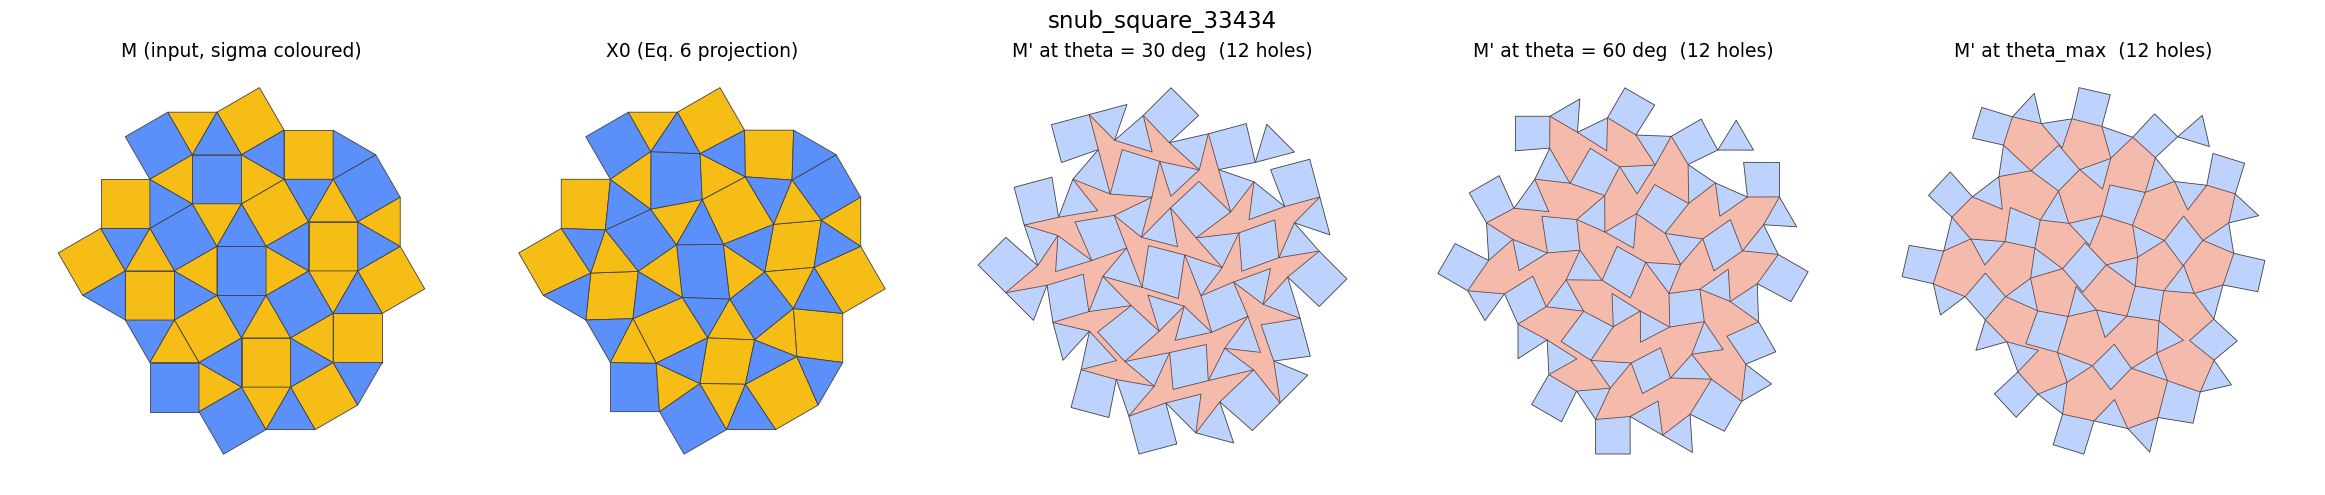
\includegraphics[width=0.48\textwidth]{results/core_validation/cases/snub_square_33434.png}\hfill
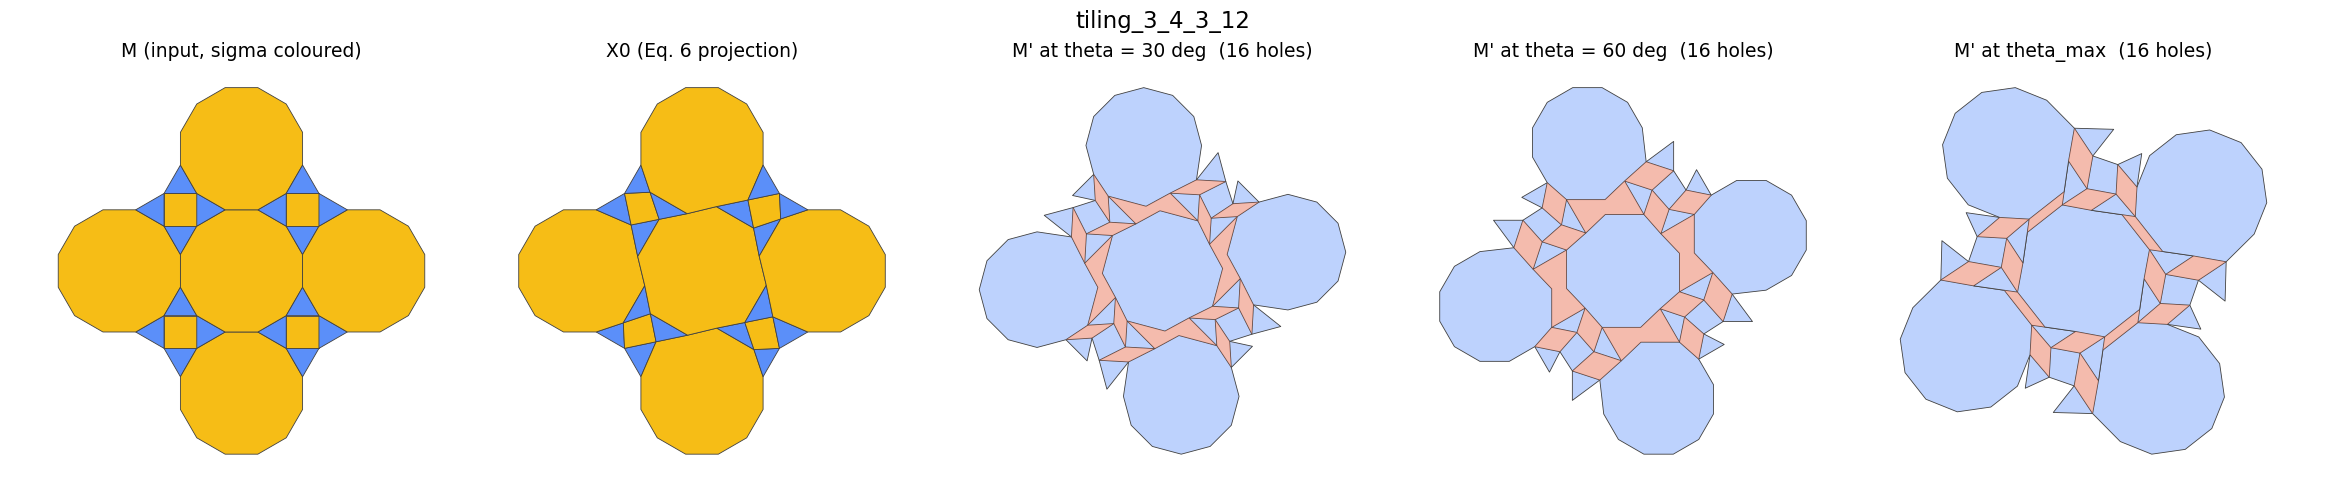
\includegraphics[width=0.48\textwidth]{results/core_validation/cases/tiling_3_4_3_12.png}
\caption{The two reference patterns that are not deployable as the Euclidean tiling. Each
figure shows $M$ coloured by $\sigma$, the Eq.~(6) projection $X_0$, and $M'$ deployed at
$30^\circ$, $60^\circ$ and $\theta_{\max}$ with the holes shaded. Left:
\fn{results/core_validation/cases/snub_square_33434.png}. Right:
\fn{results/core_validation/cases/tiling_3_4_3_12.png}. The (3,4,3,12) coordinates are not in
the paper and were reconstructed from the vertex-configuration constraints (deviation 10).}
\end{figure}

\begin{figure}[h]
\centering
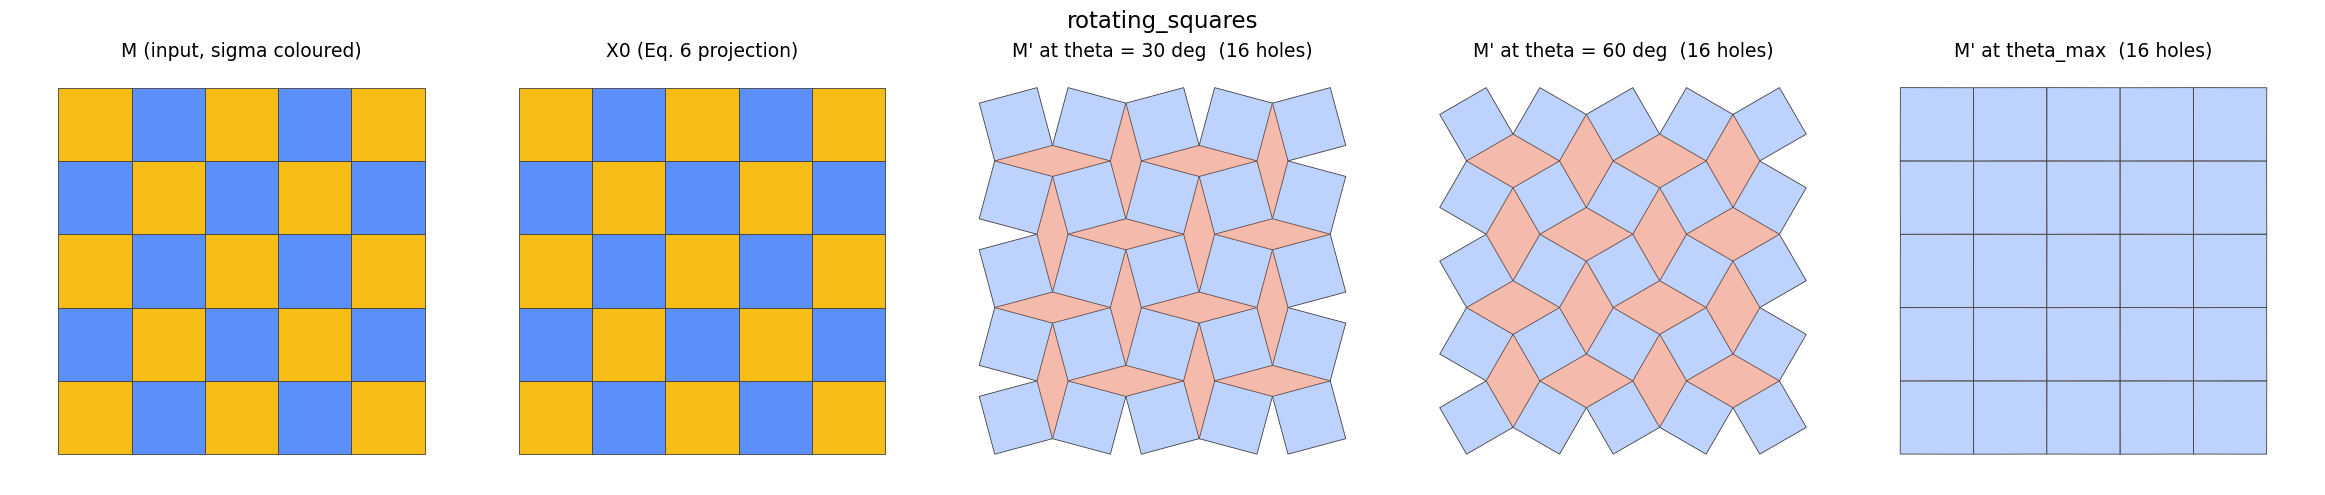
\includegraphics[width=0.32\textwidth]{results/core_validation/cases/rotating_squares.png}\hfill
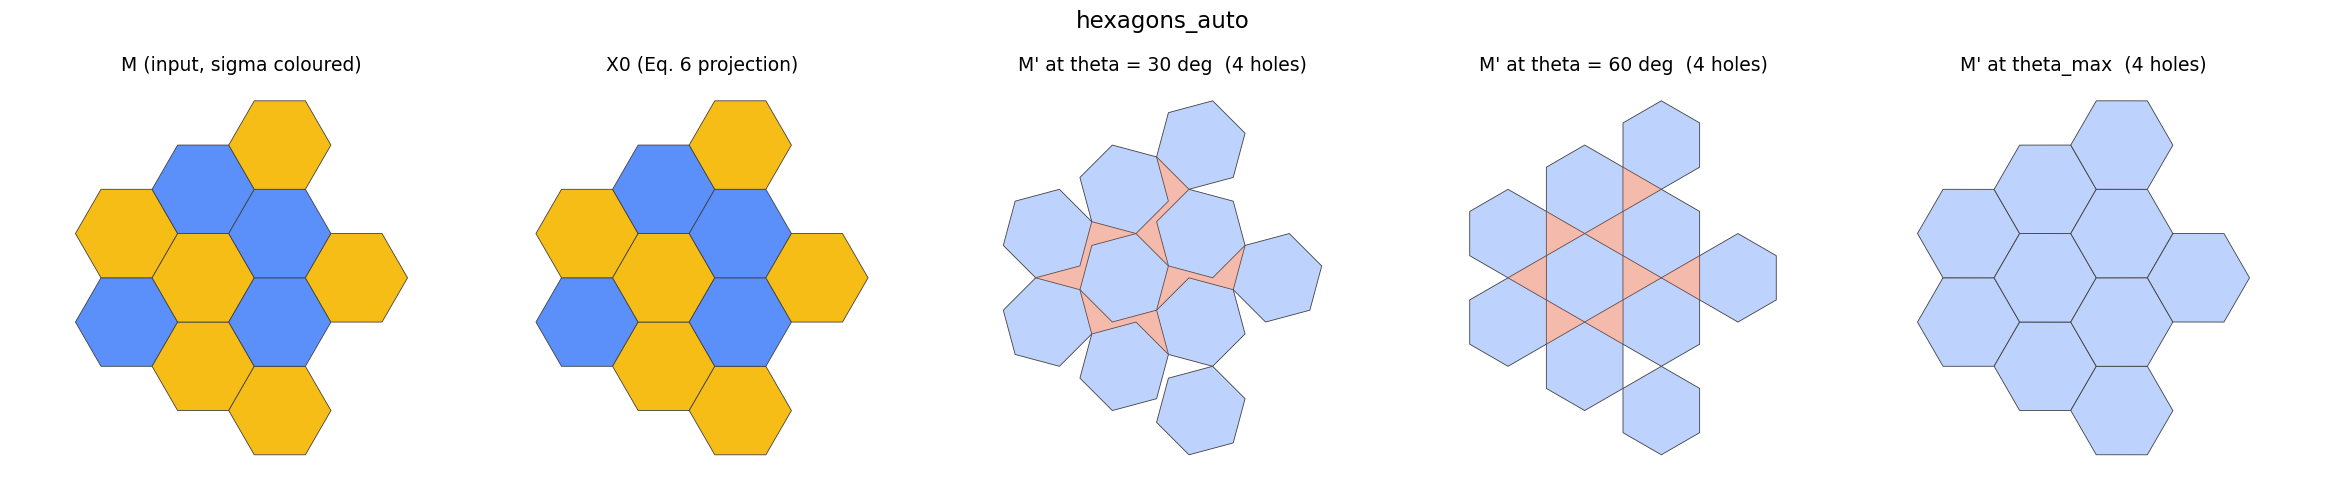
\includegraphics[width=0.32\textwidth]{results/core_validation/cases/hexagons_auto.png}\hfill
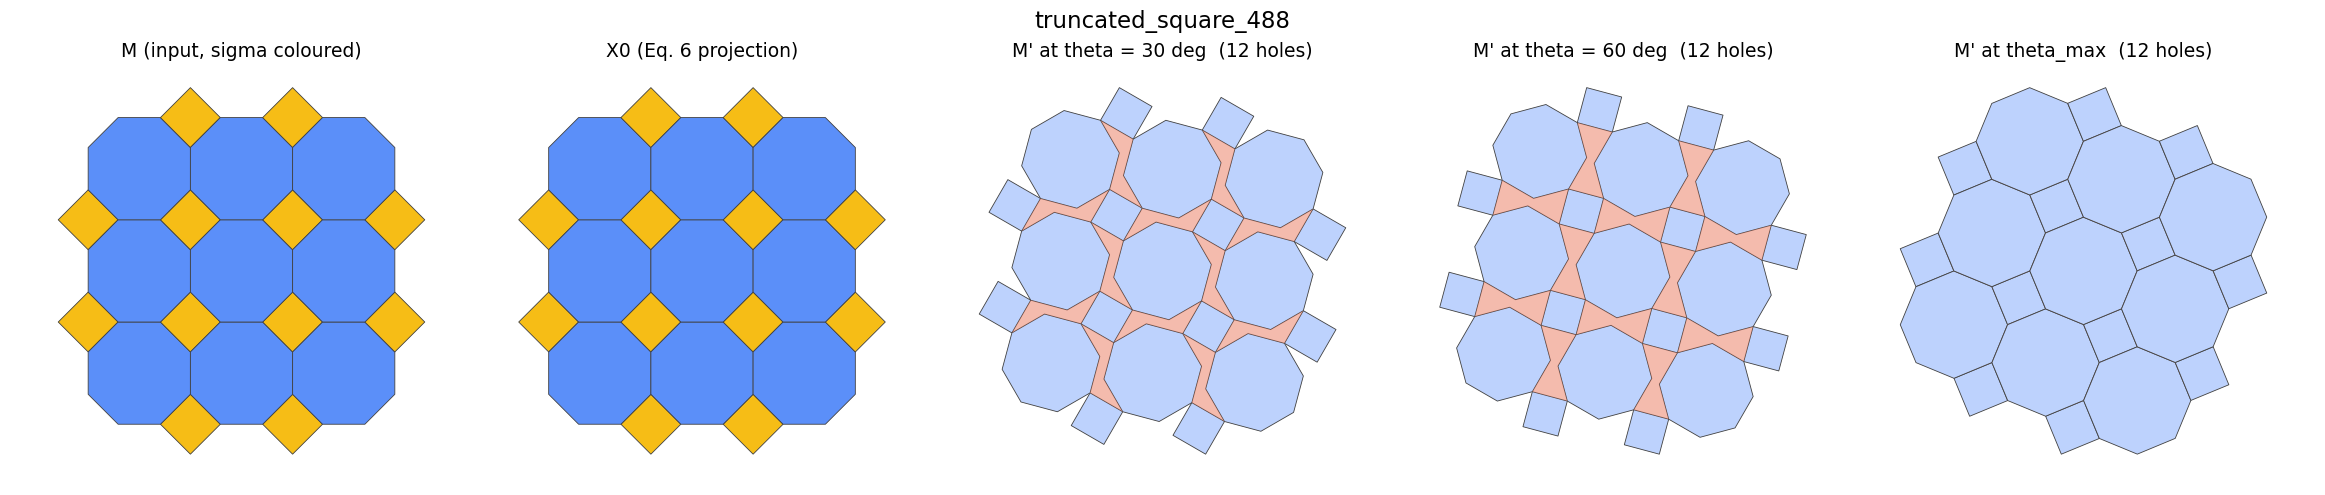
\includegraphics[width=0.32\textwidth]{results/core_validation/cases/truncated_square_488.png}
\caption{Three more reference cases: rotating squares (checkerboard $\sigma$, split-free),
the hexagonal tiling with $\sigma$ from Eq.~(1) (dual not 2-colourable, 5 split cuts), and the
4.8.8 truncated square (12 split cuts).}
\end{figure}

\subsection{The rank claim, measured}

\fn{results/core_validation/rank_claim.md}, from \fn{kiri_sweep --n 50 --seed 20260903} over
random planar graphs (Voronoi cells, Delaunay triangulations, quad-dominant edge-collapsed
Delaunay), $F$ from 115 to 2734, orientations from the paper's own Eq.~(1), fixed boundary.

\begin{table}[h]
\centering\small
\begin{tabular}{@{}lc@{}}
\toprule
2026 \S4.4 claim (prose, unproved in the paper) & holds on \\
\midrule
$\dim\mathrm{null}(\text{Eq.\ 4}) = \#\text{interior vertices} - H$ & 50 / 50 \\
$\mathrm{rank}(L) = H$ (the rows of $L$ are independent) & 50 / 50 \\
$H \le \#$interior vertices & 50 / 50 \\
\textbf{stronger relation found here:} $\dim\mathrm{null} = |E_{\mathrm{split}}|$ & \textbf{50 / 50} \\
\midrule
Remark A.1 (hinge in-degree $=$ out-degree at interior vertices) & 50 / 50 \\
Algorithm 1 $=$ split-forest partition formulation & 50 / 50 \\
hole preimages partition $E_{\mathrm{hinge}}\cup E_{\mathrm{split}}$ & 50 / 50 \\
split-cut subgraph is a forest (Remark A.4) & 50 / 50 \\
\bottomrule
\end{tabular}
\caption{Facts F15 and F22, measured. There were no violations.}
\end{table}

These are the orchestrator's three added checks, folded in later (F22):

\begin{table}[h]
\centering\small
\begin{tabular}{@{}lc@{}}
\toprule
check & holds on \\
\midrule
1a.\ $\mathbf 1^{\!\top}L$ equals the naive degree difference $\mathrm{indeg}(v)-\mathrm{outdeg}(v)$ & \textbf{0 / 50} \\
1b.\ $\mathbf 1^{\!\top}L$ equals the notch-restricted degree difference (corrected form) & \textbf{50 / 50} \\
1c.\ $\mathbf 1^{\!\top}L$ supported on boundary vertices only & 0 / 50 \\
2a.\ $L = RD$ exactly (max absolute difference 0) & \textbf{50 / 50} \\
2b.\ $\mathrm{rank}(L) = H - \dim Z$ & 27 / 27 (dense only) \\
2c.\ every $y\in Z$ gives an out-harmonic $g$, tol $10^{-9}$ & 27 / 27 \textbf{vacuously} ($\dim Z=0$) \\
3a.\ $H = |E_{\mathrm{hinge}}| - |F| + c(\Gamma)$ & \textbf{50 / 50} \\
3b.\ $H_{\mathrm{all}} = |E_{\mathrm{hinge}}| - |F| + c(\Gamma)$ (holes plus notches) & \textbf{0 / 50} \\
Eq.~(1) auto-orientation yields $c(\Gamma) = 1$ & 50 / 50 \\
\bottomrule
\end{tabular}
\caption{The three added rank checks. Check 1 as first stated is false on any patch with a
boundary, because $L$ carries a row only for an all-interior preimage; the corrected identity
is $(\mathbf 1^{\!\top}L)_v = I(v)\cdot\mathrm{indeg}(v) - \sum_{v\to w} I(w)$ with $I$ the
indicator that $K(v)$ is a hole row --- exactly the $y\equiv 1$ instance of the out-harmonic
characterization. Check 3b failing on 50/50 is the statement that notches are \emph{not}
bounded faces of $\Gamma$.}
\end{table}

Check 2c has real content only where $\dim Z > 0$, which in everything measured means the
three boundary-free torus patches. There, $\mathbf 1^{\!\top}L = 0$ exactly,
$\mathrm{rank}(L) = H-1$, $\dim Z = 1$, and the out-harmonic residuals are
$3.331\times10^{-16}$, $7.216\times10^{-16}$ and $5.551\times10^{-16}$ for
\fn{torus_squares_4x4}, \fn{torus_squares_6x4} and \fn{torus_triangles_4x4}. On those patches
the plane Euler count overshoots $H$ by exactly one, because $\Gamma$ lives on a surface of
Euler characteristic $0$: $H = |E_{\mathrm{hinge}}| - |F| + c(\Gamma) - 1$.
The Critic flagged a prose/table inconsistency in this file about check 2c; the second
Experimenter resolved it, and the file now marks row 2c ``27/27 vacuously''.

\paragraph{Facts F17 and F19.} On the same sweep, the dense null space and $X_0$ were computed
on 27 of 50 graphs, and $X_0$ was free of face--face overlap at $\theta=0$ on \textbf{0 of 27}.
The mean fraction of faces whose orientation flips in $X_0$ is 0.058; the largest vertex
displacement of the Eq.~(6) projection is 11.095 in a box of side 40. An earlier 100-graph
sweep reported 57/57 invalid with mean 5.9\,\%. \emph{Both numbers are on disk and the Critic
required both to be reported.} The worst dense solve in the sweep took 2382.611\,ms; $\dim$null
reaches 1017 on a 1052-face Voronoi patch, so optimization-in-null-space ideas are not vacuous
(F19).

\subsection{Deviations from the paper, and from the authors' code}

\fn{code/README.md} records eleven deviations. The load-bearing ones:

\begin{enumerate}[nosep,leftmargin=6mm]
\item \textbf{Algorithm 1 line 10 is incomplete}; the prose rules are implemented instead,
      which makes Alg.~1 provably identical to the split-forest formulation.
\item \textbf{Which preimages become rows of $L$.} The paper never says what happens to a
      preimage that runs into the mesh boundary. Only all-interior preimages contribute rows;
      the rest are notches open to the exterior. \emph{This is the one real mathematical
      disagreement with the authors' code} (\S4.5, F23).
\item Definition 4.1 excludes border edges, so \fn{holes_geometric} discards traced regions
      whose boundary contains an uncut border edge.
\item \textbf{Numerical rank.} The paper gives no threshold. Used:
      $\sigma_i > \max(10^{-10}\sigma_{\max}, 10^{-14})\cdot\max(\text{rows},\text{cols})$.
\item \textbf{Dense vs.\ sparse.} Dense SVD up to $N\le 1400$; above that only the rank via
      \texttt{SparseQR} with pivot threshold $10^{-9}$. K3a later showed this estimate is
      unreliable above about 700 columns (\S7.9).
\item \textbf{The barrier $B$ of Eq.~(8) has no formula in the paper.} Used:
      $B(s) = \kappa\log(1+e^{-s/\kappa})$ with $\kappa = 0.05$.
\item \textbf{$\gamma$ has no value, and a single $\gamma$ can make $\theta_{\max}$ worse.}
      \fn{optimize_collision_sweep} runs a ladder
      $\{10^{-4},10^{-3},10^{-2},3\!\cdot\!10^{-2},10^{-1},3\!\cdot\!10^{-1},1,3,10\}$ and keeps
      the best, with $T=0$ as a fallback. The regularizer is squared, following Eqs.~(6) and
      (13) rather than Eq.~(9) as printed.
\item Rounding in Eq.~(1) is projected gradient descent on the unit circle with random
      restarts, then the best of 180 evenly spaced diameters, ranked first by the number of
      components of $M'$ and then by the number of split cuts, with two repairs.
\item[9.] $\theta_{\max}$ is searched on $(0,\pi]$ by grid scan then bisection, faces shrunk by a
      relative $10^{-6}$ about their centroid.
\item[10.] The (3,4,3,12) coordinates are reconstructed; the per-cell area balance closes exactly.
\item[11.] Periodic boundaries are linear constraints on a finite patch plus one pinned vertex;
      the boundary edges are \emph{not} topologically identified.
\end{enumerate}

\subsection{Parity against the authors' native code}

\fn{baseline/native} compiles the authors' published \fn{tuttekiri} sources natively on arm64
and drives them on our JSON graphs. Three workarounds were needed, none inside
\fn{baseline/tuttekiri/}, which is read-only: Eigen is pinned to 3.4.0 by \texttt{FetchContent}
because libigl v2.5.0 and Optiz are written against the Eigen 3.x internal API; two lines of
Optiz's CMake that append a bare \texttt{-fopenmp} on AppleClang are deleted in the fetched
copy; and a $\sim$40-line \fn{emscripten/bind.h} stub is supplied whose every operation
\emph{throws}, so a silent wrong answer is impossible. \fn{bind.cpp} is excluded and replaced
by our CLI. Configure took 44\,s, build about 4 minutes.

The $\sigma\leftrightarrow$colour correspondence was \emph{measured}, not assumed: with the
naive map the deployed configurations differ by 4.5\,\% of the patch diameter; with
$\sigma=+1 \leftrightarrow$ colour 1 they agree to $2\times10^{-8}$ on every reference case,
the residual being \texttt{float} rounding in their \texttt{deploy}.

\begin{table}[h]
\centering\footnotesize
\begin{tabular}{@{}lrrrrccrrrr@{}}
\toprule
case & $E_h$ ours & $E_h$ theirs & $E_s$ ours & $E_s$ theirs & set$=$ & $H$ ours & rows theirs & res.\ in theirs & res.\ after & FK@30$^\circ$ \\
\midrule
\fn{hexagons_auto}         & 13 & 13 & 5 & 5 & yes & 4 & 28 & 1.73e+00 & 1.66e--15 & 1.3e--08 \\
\fn{kagome_3636}           & 174 & 174 & 0 & 0 & yes & 78 & 123 & 2.84e--15 & 2.30e--14 & 1.6e--08 \\
\fn{periodic_squares_4x4}  & 24 & 24 & 0 & 0 & yes & 9 & 25 & 0.00e+00 & 3.33e--15 & 1.6e--08 \\
\fn{rotating_squares}      & 40 & 40 & 0 & 0 & yes & 16 & 36 & 0.00e+00 & 1.05e--14 & 2.0e--08 \\
\fn{snub_square_33434}     & 64 & 64 & 13 & 13 & yes & 12 & 37 & 3.24e+00 & 5.99e--15 & 2.7e--01 \\
\fn{tiling_3_4_3_12}       & 40 & 40 & 4 & 4 & yes & 16 & 52 & 3.59e+00 & 6.44e--15 & 3.6e--01 \\
\fn{triangles_alternating} & 121 & 121 & 0 & 0 & yes & 33 & 58 & 2.04e--15 & 1.48e--14 & 3.9e--08 \\
\fn{truncated_square_488}  & 32 & 32 & 12 & 12 & yes & 12 & 44 & 8.31e--16 & 3.72e--15 & 1.7e--08 \\
\bottomrule
\end{tabular}
\caption{Parity, from \fn{baseline/parity.md}. $E_{\mathrm{hinge}}$ and
$E_{\mathrm{split}}$ agree \emph{exactly as sets} on 8/8, symmetric difference 0. Forward
kinematics agrees to $4\times10^{-8}$ on 8/8 when both are applied to a \emph{deployable}
embedding; the two rows with a 0.27--0.36 gap are exactly the two the reference file marks
``deployable as given: no'', and re-running them on $X_0$ gives $3.0\times10^{-8}$ and
$1.8\times10^{-8}$. Their KKT projection and our dense-SVD route compute the same least-norm
projection.}
\end{table}

\paragraph{F23 --- the one real disagreement.} \emph{Their} constraint system is strictly
stronger than ours on 2 of 8 cases. Their residual of \emph{our} $X_0$ is $1.73$ on
\fn{hexagons_auto} and $1.00$ on \fn{snub_square_33434} and $\le 4\times10^{-15}$ elsewhere;
our residual of \emph{their} $X_0$ is $\le 4\times10^{-15}$ everywhere. The cause is deviation
2: the authors build one row per \emph{vertex class} of the split-edge subgraph and do not drop
the classes that touch the boundary, and such a class still collects the hinge edges cutting
into its interior vertices. Our null space is one dimension larger on those two patterns.
The orchestrator's reasoning is that the faces around a boundary-touching component form a
\emph{path} in $\Gamma$, the exterior breaking the cycle, so no closure constraint is needed.
This was confirmed experimentally in \S7.10.

\paragraph{Orientation assignment.} Their \fn{coloring::initialized_two_face_coloring} and our
Eq.~(1) solver reach the \emph{same objective value} on 8/8 --- identical hinge and split counts
--- even on the two cases where the assignment itself differs (\fn{hexagons_auto} 9/10,
\fn{snub_square_33434} 43/53). Their routine seeds from \texttt{Eigen::Random} without seeding
\texttt{srand}, so it is deterministic per process but arbitrary.

\paragraph{$\theta_{\max}$, and F18.} Their kinematic bound equals our $\min\beta$ to
$2\times10^{-6}$ on 7/8; the exception is \fn{tiling_3_4_3_12} (2.617994 vs.\ 2.380636), where
their bound is looser and our value is confirmed by their own collision scan. Their
collision-aware $\theta_{\max}$ is \emph{wrong} on the snub square: 0.067307 against a true
first contact in 1.6919--1.7483, because their scan calls \texttt{merge\_close\_verts} with
tolerance $0.1\times$ the average edge length before the overlap test, fusing hinge duplicates
that have opened by less than that (F24). But on Eq.~(9) the direction of the error reverses:
\textbf{their} \texttt{prevent\_intersections} at published defaults (barrier 0.1, strength 10,
close 0.1) produces a snub-square pattern that \emph{our own} detector certifies to
$\theta_{\max} = \pi$, where ours could not improve $1.646137$ at any $\gamma$. On 4.8.8 the two
are level (2.353852 vs.\ 2.356196). This is F18 as corrected, and it forced the withdrawal of
the Critic's P3 headline (``Eq.~(9) achieves nothing on the snub square'') and the rule that
\emph{any margin claim must be against their code}. The likely reason for the gap: their barrier
acts on \fn{trace_hole}, a first-order collision-free quantity, while our deviation-6/7 barrier
acts on a different argument with a $\gamma$ ladder.

\paragraph{Two upstream defects found.} \fn{UnitPattern::get_holes()} dereferences
\fn{cur_edge->prev()->twin()} with no null check and segfaults on \emph{any} bounded patch, so
their hole tracer could not be run on any of the eight cases; and the
\texttt{merge\_close\_verts} artefact above. Neither is in doubt: both were found by building
and running their code.

\paragraph{Not checked.} Their hole tracer (segfault); periodic boundary conditions in their
formulation (our \fn{periodic_squares_4x4} carries no \texttt{periodic} block, so it was treated
as a bounded patch); the inverse-design pipeline (needs a 3D target); and their
\texttt{conformalize} (Eq.~13), for which we have no counterpart.

%=====================================================================
\section{Ideation}
%=====================================================================

Four Ideators ran under different personas, then a Critic. Gate 4 required each of the top five
ideas to carry a runnable kill experiment specified in code terms; it PASSED with specs
K1a/K1b/K2a/K2b/K2c/K3a.

\subsection{The geometer (\texttt{ideas/persona\_geometer.md}, 806 lines)}

\begin{table}[h]\centering\small
\begin{tabular}{@{}lp{78mm}p{56mm}@{}}
\toprule
ID & Claim & Kill experiment \\
\midrule
G1 & Every face rotates by $\omega_f = \sigma(f)\theta/2$; $Y_\theta = \cos(\theta/2)X' + \sin(\theta/2)J(CX)$, linear in $X$ & 200 graphs, 50 angles vs.\ FK; deviation $>10^{-9}$ kills \\
G2 & $J(\theta) = \cos(\theta/2)I + \sin(\theta/2)W$ with $W$ constant, so Eq.~(13) \emph{is} global conformality & 30 periodic patterns, 200 samples; distortion $>10^{-9}$ kills \\
G3 & Every edge-pair collinearity is a root of $P + Q\cos\theta + R\sin\theta = 0$ with $P,Q,R$ quadratic in $X$ & 300 graphs, closed form vs.\ bisection; $>10^{-6}$ kills \\
G4 & Holes biject with bounded faces of $\Gamma$: $H = |E_h| - |F| + c(\Gamma) = V_{\rm int} - |E_s| + (c(\Gamma)-1)$ & 500 graphs, Alg.~1's $H$ vs.\ $\Gamma$ face count \\
G5 & $\mathrm{rank}(L) = H - \dim Z$; $\dim Z \le$ \#closed communicating classes; corank $\ge 2$ achievable & 500 graphs plus a corank search over 2000 small graphs \\
G6 & $\deg_{\rm split}(v)\equiv\deg(v)\bmod 2$, so $E_{\rm split}$ is a T-join; exact $\sigma$ is polynomial (Edmonds) & 500 graphs; any parity violation kills \\
G7 & $L = A_S\Delta_h$: Tutte auxetic embeddings are split-component-averaged harmonic maps & assemble $L$ both ways; any difference kills (also kills F11) \\
G8 & There is a 3-connected planar $M$ with convex boundary whose $\Delta_h X = 0$ solution is \emph{not} an embedding & 2000 2-colourable graphs; no negative face area kills \\
G9 & The non-uniform deployment variety is cut out by cycle functionals on $\Gamma$, codimension $\le 2H$ & 100 graphs, corank vs.\ numerical mobility \\
G10 & Maximizing exact $\theta_{\max}$ over the shape space beats Eq.~(9)'s $\theta=0$ surrogate & 25 graphs; median gain below 15\,\% kills \\
\bottomrule
\end{tabular}
\end{table}

\paragraph{Self-attack.} G2 \emph{reject}: once $P_\theta = \cos(\theta/2)P_0+\sin(\theta/2)Q$
is written, the content is that a pencil $cI+sW$ is conformal iff $W$ is --- undergraduate
linear algebra; Segall et al.\ wrote ``we observe'' because the point is trivial, not because
they were stuck. G3/G10 \emph{reject}: the reduction handles collinearity of two straight edges,
but real collision-freeness is a containment problem over $O(|E'|^2)$ pairs with a
combinatorial overlap predicate relegated to ``an overlap screen'' and never analysed --- that
is where all the difficulty lives; and the headline experiment beats a baseline the submission
itself invented. G6 \emph{reject}: planar max-cut is Hadlock 1975, textbook.
The persona's own replies concede that G3's overlap screen is a genuine unresolved gap that
must be settled before commitment, and that G6's algorithmic half is weak.

\paragraph{Numbers it ran.} Opening angles equal $\theta$ to 12 decimals on a $5\times5$ patch;
potential closure residual $1.8\times10^{-15}$; closed form vs.\ rigid-motion FK
$2.0\times10^{-15}$; edge-length drift $1.1\times10^{-15}$;
$H = |E_h|-|F|+c(\Gamma)$ on a $6\times6$ patch with \textbf{400 random $\sigma$}: 0/400
failures, while the version without $c-1$ fails 400/400, with $c(\Gamma)$ reaching 10 and
$V_{\rm int}-|E_s|$ going as low as $-7$ while $H = 2$; the T-join parity: 0 failures over the
same 400 trials $\times$ 25 interior vertices; Remark A.1: 0 failures.

\subsection{The optimizer (\texttt{ideas/persona\_optimizer.md}, 825 lines)}

Ten ideas, of which the distinct ones are: a geometry-aware $\sigma$ objective in place of
max-cut; \textbf{idea 1}, $J(\theta) = \cos(\theta/2)I+\sin(\theta/2)K$ with $K$ constant and
linear in $X$, so $\{K(X)\}$ is an affine subspace; \textbf{idea 2}, total hole area
$A(\theta) = q(\cos\theta - 1) + r\sin\theta$, whence a second gap-free angle
$\theta_{\rm closed} = 2\arctan(r/q) = 2\arctan\!\big(\mathrm{tr}\,K/(1-\det K)\big)$;
\textbf{idea 3}, contact events as harmonic roots; \textbf{idea 4}, range maximization as a QCQP
with a Shor/Burer--Monteiro certified upper bound; \textbf{idea 5}, the deployability defect
$D(\sigma)$ is \emph{not} monotone in $|E_{\rm split}|$; \textbf{idea 6}, the dual is planar so
max-cut here is polynomial (Orlova--Dorfman 1972 / Hadlock 1975); \textbf{idea 7}, a local
sparse basis for $\ker L$; \textbf{idea 8}, the complex torus variety
$\{Wz = 0, |z_f| = 1\}$; \textbf{idea 9}, low-rank QCQPs for inverse design; \textbf{idea 10},
hole size and balance do not correlate with auxetic quality --- the isotropy defect and
$\dim\{K(X)\}$ do.

\paragraph{Self-attack.} Idea 1 \emph{reject}: two lines following immediately from the
kinematic model the authors already state, and the authors clearly computed
$\partial J/\partial\theta|_0$ to derive Eq.~(13), so they had the linearity in front of them.
Idea 8 \emph{reject}: writing planar rotations as unit complex numbers so loop closures become
linear is the classical complex-vector loop-equation method taught since the 1950s, and
Kapovich--Millson says such sections realize arbitrary varieties, so the structure buys no
tractability. Idea 2 \emph{reject}: $A(\theta)=0$ is only \emph{necessary} for closure, and the
persona concedes signed areas cancel under overlap.

\paragraph{Numbers it ran.} \textbf{None.} Verbatim: ``Nothing in this file was executed. No
code was built or run; every number quoted is a prediction.''

\subsection{The rigidity theorist (\texttt{ideas/persona\_rigidity.md}, 678 lines)}

Ten ideas, the load-bearing ones being: \textbf{1}, mobility $m = \dim\ker A - c(\Gamma)$ for the
$2b_1(\Gamma)\times|F|$ closure matrix $A$, with $\sigma\in\ker A$ iff uniformly deployable
(this is U4); \textbf{2}, $m(0) > m(\theta) = \text{const}$ on the open interval, so the flat
state is a branch point (U5); \textbf{3}, $Y_\theta = \cos(\theta/2)C(X)+\sin(\theta/2)S(X)$
with $C,S$ linear, so with $\tau = \tan(\theta/2)$ every contact event is a quadratic root
(U3); \textbf{4}, the periodic Jacobian pencil; \textbf{5}, $A(\theta)$ is a linear matrix
pencil so bifurcation angles are generalized eigenvalues; \textbf{7}, the 2-core identity
$m = |F\setminus\mathrm{core}_2| + (\dim\ker A_{\rm core} - c)$; \textbf{9}, range maximization;
\textbf{10}, a second-order prestress certificate for which flat-state flexes extend.

\paragraph{Self-attack.} Idea 1 \emph{reject}: a planar body-and-pin compatibility condition
being a circulation condition on the joint graph is instant-centre kinematics, and the ``three
collinear pins'' corollary is Aronhold--Kennedy (1872). Idea 3 \emph{reject}: rational
trajectories in $\tan(\theta/2)$ is the Weierstrass substitution. Idea 2 \emph{reject}: the
claim rests on a numerical rank at $\theta = 10^{-6}$ vs.\ $\theta=0$ with an unjustified,
never-varied tolerance, and the persona's own data contain an unexplained counterexample.

\paragraph{Numbers it ran} (its own \fn{ideas/rigidity_rig_check.cpp}, compiled against the core
sources, 21 graphs). V1: $Y_\theta = \cos(\theta/2)C+\sin(\theta/2)S$ to
$6\times10^{-15}$ at scale $\sim6$ on 21/21, with $C,S$ fitted from two angles and predicted at
five. V2: $m = \dim\ker A - c(\Gamma)$ agrees with $3|F| - \mathrm{rank}(R) - 3c$ on 21/21 at
both $X_{\rm ini}$ and $X_0$. V3: on $X_{\rm ini}$, $\|A\sigma\| \in [3.2, 11]$ with hole
residuals in $[0.65, 3.1]$; on the solved $X_0$, both $< 2\times10^{-14}$, 21/21. V4: mobility
drops discontinuously at $\theta=0$ on \textbf{20/21} --- squares $5\times5$ $10\to1$, kagome
$18\to7$, periodic squares $4\to1$, a Delaunay patch $26\to19$ --- the triangle tiling being the
one exception, keeping $m=9$. Measured mobilities on solved embeddings: 1--3 on Voronoi (many
split cuts) up to 19--26 on Delaunay. \emph{These last figures were later shown by K3a to be
population-specific and must not be quoted as general.}

\subsection{The adversary (\texttt{ideas/persona\_adversary.md}, 1222 lines)}

Ten ideas: \textbf{A1}, for split-edge pairs $P+Q=0$ so the only other root is $\tau^*=-R/P$,
and Eq.~(9) constrains only $R$ --- its false-negative rate is computable and unknown;
\textbf{A2}, the \emph{no-locking lemma} $\sigma\in\ker A(Y_\theta)$ for all $\theta$, so the
uniform branch never dead-centres and \emph{every stop is a contact}, plus the pencil and the
claim that bifurcations occur inside the range; \textbf{A3}, fully closed iff all first-contact
roots coincide; \textbf{A4}, a locality theorem giving an $O(n)$ active set; \textbf{A5},
$\nu(\theta)$ as a closed-form rational function of two invariants of $W$; \textbf{A6}, the
2-core identity, with the prediction that mobility 19--26 is a dangling-face artefact and
$m_{\rm core}$ is 1--3; \textbf{A7}, $\mathrm{rank}(L) = H - \dim Z$; \textbf{A8}, Eq.~(2) is
sufficient but not necessary; \textbf{A9}, branch counting by deflating the uniform branch;
\textbf{A10}, the usable region $U(\varepsilon)$ can have $\dim U < \dim\mathbb X$ and can be
\emph{empty} for every $\varepsilon>0$ while $\dim\mathbb X > 0$.

\paragraph{Self-attack.} A1 \emph{reject, borderline}: the contribution is that a first-order
test misses second-order events, which is the definition of a first-order test, and the
empirical claim is measured against the submission's own reconstruction of an energy whose
$B$, $\gamma$ and diameter rule are unspecified --- ``a good bug report and a poor paper''.
A2 \emph{reject}: the no-locking lemma is immediate (the path exists, so it has a tangent), and
a rank drop is only \emph{necessary} for a bifurcation (Connelly--Servatius), so the
``bifurcation spectrum'' is a spectrum of candidates. The persona calls this ``devastating and
correct''. A6 \emph{reject, decisively}: the 2-core reduction is the first step of every
rigidity-percolation implementation; ``Fair, and I do not have the mechanism''.

\paragraph{Numbers it ran.} None; it explicitly attributes every numeric claim to another
persona. Its own empirical work was a verbatim web-search log: 8 queries and 2 fetches, of
which the Dang 2021 PDF failed to extract and the Jiang \& Choi 2026 HTML was retrieved and
confirmed to contain no $\cos/\sin$ parametrization, no half-angle theorem, no closed-form
$\theta_{\max}$ and no conformality analysis.

\subsection{The convergent bundle, and the Critic's ranking}

\fn{ideas/ranking.md} (706 lines, 24 deduplicated ideas) opens with four facts from Phase 2
that no persona had.

\begin{description}[leftmargin=8mm,style=nextline,nosep]
\item[P1.] \emph{The design space and the collision problem have the same source: split cuts.}
$\dim\mathrm{null} = |E_{\rm split}|$ (F15) and $\theta_{\max} = \min_i\beta_i$ exactly on every
split-free pattern, strictly smaller as soon as split cuts exist (F18; snub square 1.646 vs.\
3.384). So a pattern has a nontrivial shape space \emph{iff} it has split cuts, and a non-local
collision deficit \emph{iff} it has split cuts. On the pure hinge case there is nothing to do.
\item[P2.] \emph{The paper's own pipeline returns a geometrically invalid embedding.} On the
random graphs of the title, while the eight authored tilings are fine. ``The method works on
the tilings the paper shows and fails on the arbitrary planar graphs its title claims.''
\item[P3.] \emph{Eq.~(9) fails outright on named tilings} --- \textbf{later withdrawn} after the
baseline parity (F18).
\item[P4.] The added rank checks: $L = RD$ 50/50, $\mathrm{rank}(L) = H - \dim Z$ 27/27,
periodic $\mathrm{rank}(L) = H-1$ on three tori, $H = |E_h|-|F|+c(\Gamma)$ 50/50 with
$c(\Gamma)=1$ on 50/50. It also caught the prose/table inconsistency about check 2c and the fact
that A8's existence half is already published as 2025 Fig.~10.
\end{description}

The Critic's verdict on the convergent bundle as handed over (B1+B2+B3+B4+B11) is
\textbf{``a collection of paragraphs''}, on two grounds: two of its five claims have a named
living competitor (Acu\~na et al.\ 2022, and Tay--Whiteley for the mobility half), and
``the bundle's load-bearing theorem, if you write it out, is a definition'' --- uniform
deployability says every hinge opens by $\theta$, $\Gamma$ is bipartite by construction, so
face rotations are pinned up to a global rotation, and there is nothing to prove. Its verdict:
an excellent \S3, four pages of machinery that licenses a real result, but not the result.

\begin{table}[h]\centering\small
\begin{tabular}{@{}p{6mm}p{32mm}p{112mm}@{}}
\toprule
& Idea & Hostile verdict, in one line, and the outcome \\
\midrule
R1 & the usable shape space & \textbf{PURSUE} --- first commitment. ``The only idea in all four files where the kill experiment cannot leave you with nothing.'' The reviewer's ``Weierstrass substitution'' charge lands halfway; the defensible claim is the \emph{finite, complete, exactly enumerable} constraint list. \\
R2 & exact contact calculus with an $O(n)$ active set & PURSUE-IF-KILL-PASSES, but not separately: it is R1's \S4. ``Commit to K2c before anyone writes the word theorem.'' \\
R3 & bifurcation spectrum with a second-order certificate & PURSUE-IF-KILL-PASSES. ``The only question in the four files whose answer nobody knows.'' Killed by K3a. \\
R4 & achievable periodic Jacobians / designable Poisson family & PURSUE-IF-KILL-PASSES, as the \emph{second} paper. Risk: if the achievable rank is 1 the set is a curve and there is nothing to design. \\
R5 & the orientation objective is wrong & PURSUE-IF-KILL-PASSES, third tier; it belongs inside R1 as the section explaining why the shape space is the size it is. \\
\bottomrule
\end{tabular}
\caption{The Critic's top five and its verdicts. Just below the line: B14 (2-core) is not a
paper but is ``the first thing to run''; B20 (fully closed as root coincidence) and B5
(periodic corank) are cheap and decisive but carry no paper; B9 (non-uniform deployment) is
excluded by 2025 Fig.~10.}
\end{table}

The Critic's own honesty note: it ran no code and no searches, it read
\fn{notes/field_tutte.md} only in the parts bearing on injectivity and relied on the personas'
citations for the other two tables, and \fn{github.com/segaviv/tuttekiri} had not been retrieved
by anyone at that point --- so every ``beats the baseline'' claim was against a reconstruction.
Retrieving and building that code became step zero, and it produced F18, F23 and F24.

\subsection{Decisions D5--D8}

\begin{description}[leftmargin=8mm,style=nextline,nosep]
\item[D5 (S2, following the Critic).] First commitment $=$ R1, ``the usable shape space'':
certified valid and range-optimal embeddings within the Tutte auxetic null space, where
Eq.~(6) is invalid (F17) and Eq.~(9) is $\gamma$-fragile (F18). Load-bearing theorem: since
$Y_\theta$ is trig-linear in $X$, $U(\varepsilon)$ is a basic semialgebraic set cut out by
quadrics with a finite complete constraint list, completeness via the no-locking lemma.
Fallbacks in order: R3, R4, R2 standalone, R5, B20. A8 dropped (F20).
\item[D6 (S2 22:10, after K1a and K3a).] R1 stays, but its core algorithm becomes \emph{joint}
orientation plus geometry: choose $\sigma$ by minimizing the deployability defect $D(\sigma)$ at
$X_{\rm ini}$, then project and range-optimize with exact contact roots. Headline claim to test
(K5): max-cut $\sigma$ gives 0/200 valid; defect-minimizing $\sigma$ gives a substantial
fraction.
\item[D7 (S2 23:30, after K2b FAIL).] Drop range optimization as the headline. The deliverable
becomes a \emph{characterization}: exact closed-form deployment range and validity certificate
for arbitrary-graph kirigami (T1--T6, to be scaled to $\ge500$ graphs in Phase 9), the emptiness
result (K1a), the Eq.~(9) false-negative rate (K1c), and the periodic rank and hole-count
corrections (F14/F22). If K5 passes, add the algorithm.
\item[D8 (S2 02:30, human directive ``go to a different hypothesis'' after K6's 7.5\,\% interim).]
Keep the characterization core. The \emph{constructive} half pivots from random graphs, where
the space is generically empty, to \textbf{periodic} patterns where it is usable: R4 achievable
periodic Jacobians, $J(\theta) = \cos(\theta/2)I + \sin(\theta/2)K$ with $K$ affine in the null
space so the achievable set is an affine subspace --- algorithm: target $K$, linear solve,
certificate-maximal member --- together with B20, the closed-form second fully-closed angle from
the hole-area harmonic. Kill experiment K7 was spawned; K6 is to be logged as a dead end once
its final report is in.
\end{description}

%=====================================================================
\section{Theory: T1--T7 and five rounds of checking}
%=====================================================================

\fn{derivations/core.md} (1971 lines) tags every step \textbf{[D]} definition, \textbf{[F]}
cited fact, \textbf{[A]} an algebraic step a Checker can verify by hand, or \textbf{[N]} a
numeric check actually run with the program named and the result quoted. Nothing is asserted
without one of the four. \fn{derivations/check.md} (1154 lines) is the Checker's independent
review; it saw only the \emph{statements}, the code, \fn{STATE.md} F1--F24 and
\fn{notes/paper_2026.md}, never the Deriver's reasoning, and re-derived every algebraic step by
hand from the code's own sign convention.

\subsection{T1 --- trig-linear deployment}

\emph{Hypotheses}: $M$ embedded planar, $\sigma$ given, $\Gamma$ connected, $X$ satisfying
Eq.~(2) on a cycle basis of $\Gamma$, rigid faces. No genericity is used.

The hinge constraint is a discrete potential equation on $\Gamma$: with $t_f = 2sJu_f$, the
deployed position of the copy $(v,f)$ is $y_{(v,f)} = c\,x_v + s\,J(2u_f - \sigma_f x_v)$, whence
\[
\boxed{\;Y_\theta = \cos(\theta/2)\,C + \sin(\theta/2)\,S,\qquad
C_{(v,f)} = x_v,\quad S_{(v,f)} = J\big(2u_f - \sigma_f x_v\big)\;}
\tag{T1.5}
\]
with $u_f = \sum_{e\in \mathrm{path}_T(f_0\to f)} \sigma_{\mathrm{head}(e)}\,x_{\mathrm{src}(e)}$
a fixed signed sum of rows of $X$ with coefficients in $\{0,\pm1\}$ determined by $\Gamma$,
$\sigma$ and the spanning tree alone. Hence $C$ and $S$ are \emph{linear in $X$}, and the value
of $u_f$ is tree-independent exactly when $X\in\mathbb X$.
Corollaries: every vertex traces a centred ellipse whose semi-axes are the singular values of
$[C_{(v,f)} \mid S_{(v,f)}]$ (T1.A); split duplicates are equal translates (T1.B); a hinge opens
by exactly $\theta$ (T1.C); faces are rigid (T1.D).
Measured: the closed form matches \fn{kinematics.cpp::deploy()} at eight angles on 30 graphs to
$1.42\times10^{-14}$; the opposite sign convention fails by $O(1)$.

\subsection{T2 --- no locking}

\emph{Statement.} For every $X\in\mathbb X$ and every $\theta\in\mathbb R$,
\[
\boxed{\,A(Y_\theta)\,\sigma = 0\,}
\]
where $A(\theta)_z(\omega) = \sum_{e\in z}\varepsilon_e(\omega_{h(e)} - \omega_{t(e)})J p_e(\theta)$
is the $2b_1(\Gamma)\times|F|$ circulation map of the body-and-pin model. Consequently the
uniform branch is a real-analytic one-parameter motion defined for all $\theta$, with nowhere
vanishing non-rigid velocity, and \textbf{it never reaches a kinematic dead centre: every
termination of deployment is a contact event.} $A(\theta)$ is moreover a linear pencil, since
$p_e(\theta)$ is affine in $(c,s)$.
This is the lemma that makes T4's candidate list \emph{complete} rather than merely necessary.
Measured: pin residual $1.3\times10^{-14}$ over 22\,392 hinge evaluations at random
$\theta\in[-4,4]$; $\|A(Y_\theta)\sigma\|_\infty/\|A\|_\infty \le 1.0\times10^{-14}$ over 480
assembled matrices including $\theta=0$; pencil identity $4.0\times10^{-15}$.

\subsection{T3 --- harmonic predicates}

\emph{Statement.} Along the uniform branch every orientation, dot-product and squared-length
predicate built from $M'$ vertices is a \emph{first harmonic}
\[
h(\theta) = p + q\cos\theta + r\sin\theta
\]
whose coefficients are \emph{quadratic forms in $X$}. Explicitly, with
$C_{ab} = C_b - C_a$ and $S_{ab} = S_b - S_a$ and using
$c^2 = (1+\cos\theta)/2$, $s^2 = (1-\cos\theta)/2$, $cs = (\sin\theta)/2$:
\[
\det(Y_b - Y_a, Y_w - Y_a):\quad
\begin{aligned}
p &= \tfrac12[\det(C_{ab},C_{aw}) + \det(S_{ab},S_{aw})],\\
q &= \tfrac12[\det(C_{ab},C_{aw}) - \det(S_{ab},S_{aw})],\\
r &= \tfrac12[\det(C_{ab},S_{aw}) + \det(S_{ab},C_{aw})].
\end{aligned}
\]
Analogous triples hold for $\langle\cdot,\cdot\rangle$ and $\|\cdot\|^2$; inside a face
$q = r = 0$, so signed areas are constant in $\theta$.
With $\tau = \tan(\theta/2)$,
\[
(1+\tau^2)\,h(\theta) = g(\tau) := \underbrace{(p+q)}_{C} + \underbrace{2r}_{B}\,\tau + \underbrace{(p-q)}_{A}\,\tau^2 ,
\qquad
\tau = \frac{-r \pm \sqrt{q^2+r^2-p^2}}{p-q},
\]
real roots iff $p^2 \le q^2+r^2$; the discriminant is a quartic in the null-space coordinates.
The $\tau$ chart is singular at $\theta=\pi$, so \fn{harmonic_roots} uses the amplitude/phase
form (\texttt{atan2} plus \texttt{acos}) instead.
Measured: 3.6e--15 relative over 12\,345 samples; every reported root satisfies $h=0$ to
8.4e--14 and the real-root criterion is exact (971 of 3\,682 harmonics correctly reported
rootless). K1b independently confirms the whole structure to $4.18\times10^{-12}$ over
207\,096 triples.

\subsection{T4 --- contact calculus}

\emph{Standing hypotheses of T4--T6}, made explicit in round 5: every face polygon is
\textbf{simple}. (With \texttt{POS} alone, 5 of 873 local tests failed, all on self-intersecting
faces.)

\textbf{T4.2 (completeness).} A contact implies a vertex of one face lies on the other's
boundary, so the candidate list of ordered (vertex, edge) pairs misses nothing. This is where
T2 is consumed.

\textbf{T4.2$''$ (exact $\Theta_{\max}$).} $\Theta_{\max}$ is \textbf{not} the minimum over
harmonic roots. A root can be a \emph{graze} --- a tangency without a crossing. The correct
procedure is an interval scan: take the complete contact set $\mathcal C(X)$, walk the gaps
between consecutive candidate angles, and return the left endpoint of the first gap whose
\emph{midpoint} has an interior overlap. Interior overlap is an \emph{open} condition in
$\theta$, so the overlap set has no isolated points and the scan cannot skip one.
\fn{hexagons_auto} grazes at $\pi/3 = 1.047198$ and does not overlap until
$2\pi/3 = 2.094395$.

\textbf{T4.4 ($\beta$ as a special case).} $\beta_e = 2\pi - \alpha_f - \alpha_g$ is always in
$\mathcal C(X)$, and on split-free patterns
\[
\Theta_{\max} = \min\big(\min_e \beta_e,\ \pi\big),
\]
the cap being necessary --- the triangle tiling has $\min\beta = 4\pi/3 > \pi$. The $\le$
direction is derived; the $\ge$ direction is \textbf{measured only} (8 split-free patterns to
$8.88\times10^{-16}$), and carries that tag.

\textbf{T4.5 (broad phase).} In the face's own frame the per-face translation cancels and
$S_u - \bar g_f = -\sigma_f J(C_u - \bar g_f)$, so the two columns are orthogonal and of equal
norm: the trajectory is a \emph{circle} and the swept radius is
$\max(\|x\|,\|\chi\|) = \|x_u - \bar x_f\| $ \emph{exactly}. The round-1 $\sqrt2$ correction is
therefore \textbf{withdrawn}; applying it makes the pruning looser, not sounder. The $\sqrt2$
is real only for the \emph{absolute} trajectory, a genuine ellipse, which no pruning uses. The
broad phase pairs this exact radius with a \emph{moving-centroid} distance test; the
flat-centroid variant is unsound in principle, because deployment contracts centroid distances
while face radii stay fixed.

\subsection{T5 --- the usable region, and the certificate}

\textbf{T5.1.} Positive orientation is $|F|$ strict quadratic inequalities, a basic open
semialgebraic set --- and it is \emph{not} a validity certificate. Reproduced by the Checker:
\textbf{51 of 70} positively-oriented shape-space samples have $\Theta_{\max} = 0$; a
counterexample is saved at
\fn{derivations/check_failures/T5_1_positive_orientation_zero_range_hexagons.json}.

\textbf{T5.2a.} $U(\varepsilon) = \{X\in\mathbb X : \text{all faces positively oriented},\
\Theta_{\max}(X)\ge\varepsilon\}$ is semialgebraic, by Tarski--Seidenberg applied to a
first-order formula with polynomial atoms. The honest framing, which both agents adopted, is
that the content is the \emph{explicit description}, not semialgebraicity.

\textbf{T5.2b$'$ --- the certificate.} The final form, after three rounds of correction:
\[
\boxed{\ \mathrm{VALID}(\varepsilon)\;=\;
\mathrm{POS}\ \wedge\ \mathrm{NOOVERLAP}(\theta_1 = \varepsilon/2)\ \wedge\ \mathrm{NOROOT}(\varepsilon)
\quad\Longrightarrow\quad \Theta_{\max}\ \ge\ \varepsilon .\ }
\]
\texttt{POS} is all face signed areas $>0$ at $\theta=0$; \texttt{NOOVERLAP} is \emph{one} exact
polygon--polygon test at the single interior angle $\varepsilon/2$; \texttt{NOROOT} is no
admissible deflated root in $(0,\varepsilon)$ over the candidate list minus the
identically-zero harmonics. The $\theta = 0$ overlap test is \textbf{withdrawn}: at $\theta=0$
the two copies of every split edge coincide and adjacent faces touch along whole shared edges,
so it is \emph{degenerate}, not merely different. The proof is a connectedness argument --- the
overlap set $O$ is clopen in $(0,\varepsilon)$, and overlap status can change only at a
candidate root --- and it \emph{implies} embeddedness rather than assuming it.

\textbf{The $\tau=0$ deflation, in three classes.} With $A = p-q$, $B = 2r$, $C = p+q$:
\begin{itemize}[nosep,leftmargin=6mm]
\item $C\ne0$: class 1, the generic case.
\item $C = 0$, $B\ne0$: class 2, a \emph{simple} root at $\theta=0$, deflated away.
\item $C = 0$, $B = 0$, $A\ne0$: class 3, $h = p(1-\cos\theta)$, a \emph{double} root at
      $\theta=0$ and, by Lemma T5.1e, of constant sign on $(0,\pi)$ --- never a contact, atom
      \texttt{true}.
\item $A = B = C = 0$: a permanent incidence, struck by an identity test
      $|p|+|q|+|r| \le \mathrm{tol}\cdot\mathrm{scale}$ \emph{before} classification, so it is
      not a candidate of any class.
\end{itemize}
$C = 0$ is \emph{not} a degeneracy: it holds identically on the whole shape space for every
permanent incidence and every split-edge duplicate pair. Without the deflation the flat-state
root leaks in at $\sim10^{-8}$ and every pattern with split cuts reports $\Theta_{\max}=0$.

\textbf{T5.3 --- Eq.~(9)'s exact blind spot.} For a split-edge pair,
$(1+\tau^2)h = 2\tau(r + p\tau)$ with
\[
p = -\sigma_f\det(d,\Delta u),\qquad q = -p,\qquad r = \langle d,\Delta u\rangle .
\]
So $h'(0) = r$: Eq.~(9) certifies $r>0$ and \emph{nothing else}. The second root
$\tau^* = -r/p$ is positive iff $p<0$, i.e.\ iff $\sigma_f\det(d,\Delta u)>0$ --- a
\emph{second}-order quantity Eq.~(9) is blind to by construction. Verified over 4\,300
split-edge samples: $p$ to 3.0e--13, $q=-p$ to 3.0e--13, $r$ to 1.9e--14,
$h(2\arctan(-r/p)) = 0$ to 5.4e--14; the algebraic precondition $r>0\wedge p<0$ fires on
\textbf{871 of 4\,300} samples (20\,\%).

\subsection{T6 and T7}

\textbf{T6} gives the softmin bound $\min - \log|\mathcal A|/\beta \le \Theta_{\rm soft} \le \min$
and exact root gradients by implicit differentiation:
$\partial_i p + \cos\theta\,\partial_i q + \sin\theta\,\partial_i r + h'(\theta)\partial\theta/\partial t_i = 0$
with $h'(\theta) = -q\sin\theta + r\cos\theta$. Verified against central differences of the root
recomputed from scratch: worst relative error $3.9\times10^{-7}$ at $\Delta = 10^{-5}$ over
2\,160 (pair, coordinate) samples on 12 graphs.

\textbf{T7} is the rank and periodic block: $L = R\,D$; $\mathrm{rank}(L) = H - \dim Z$ with $Z$
out-harmonic; $\mathbf 1^{\!\top}L = 0$ and $\mathrm{rank}(L) = H-1$ in the periodic case; and
$H = |E_{\mathrm{hinge}}| - |F| + c(\Gamma)$. All six sub-items are VERIFIED by the Checker on
its own 16-case corpus, with $L = RD$ recomputed from its own $R$ and $D$ to \emph{exactly} 0
difference, and $H = |E_h|-|F|+c(\Gamma)$ on 16/16 corpus \textbf{and 398/398 random-$\sigma$}
cases.

\subsection{What is proved, what is measured, what is conjecture}

\begin{table}[h]\centering\small
\begin{tabular}{@{}p{14mm}p{92mm}p{48mm}@{}}
\toprule
\# & Statement & Status \\
\midrule
T1 & $Y_\theta = \cos(\theta/2)C+\sin(\theta/2)S$, $C,S$ linear; path-independence $\Leftrightarrow$ Eq.~(2) & \textbf{proved} $+$ [N] 1.4e--14 \\
T1.A--D & ellipse; split duplicates are equal translates; hinge opens by $\theta$; faces rigid & \textbf{proved} $+$ [N] \\
T2 & $A(Y_\theta)\sigma = 0$ for every $\theta$; no locking; $A(\theta)$ is a pencil & \textbf{proved} $+$ [N] 1.8e--14 \\
T3 & harmonic predicates, quadratic coefficients, $\tau$-quadratic roots & \textbf{proved} $+$ [N] (K1b 4.18e--12) \\
T4.2 & contact $\Rightarrow$ a vertex on the other's boundary; the list is complete & \textbf{proved} \\
T4.2$''$ & exact $\Theta_{\max}$ by candidate $+$ interval scan & \textbf{proved} $+$ [N] 2.1e--6 vs.\ bisection \\
T4.4 & $\Theta_{\max} = \min(\min_e\beta_e,\pi)$ on split-free patterns & \textbf{proved} ($\le$) $+$ \textbf{measured only} ($\ge$), 8.88e--16 \\
T4.5a & exact broad phase with the moving centroid & \textbf{proved} \\
T4.5b$'$ & in the face frame the swept radius is exactly the flat circumradius & \textbf{proved} $+$ [N] 3.11e--15 \\
T5.1 & positive orientation is $|F|$ quadratics, and is \emph{not} a certificate & \textbf{proved} $+$ [N] 51/70 counterexamples \\
T5.2a & $U(\varepsilon)$ semialgebraic & \textbf{proved} \\
T5.2b$'$ & $\mathrm{POS}\wedge\mathrm{NOOVERLAP}(\varepsilon/2)\wedge\mathrm{NOROOT}$ is an \emph{inner} approximation & \textbf{proved} $+$ [N] 0 violations \\
T5.1e & class 3 $h = p(1-\cos\theta)$ has constant sign on $(0,\pi)$ & \textbf{proved} (round 3) \\
T5.2b.1/.2 & quantifier-free atom list of degree $\le 4$ with the three-class deflation & \textbf{proved} $+$ [N] 0 / 2\,145\,387 \\
T5.3 & the exact Eq.~(9) false-negative condition & \textbf{proved} $+$ [N] 4.4e--15 \\
T6.2 & exact root gradients by implicit differentiation & \textbf{proved} $+$ [N] 3.9e--7 \\
T7 & $L=RD$; $\mathrm{rank}(L) = H-\dim Z$; periodic $\mathbf 1^{\!\top}L=0$; $H = |E_h|-|F|+c(\Gamma)$ & \textbf{proved modulo F11} $+$ [N] \\
\bottomrule
\end{tabular}
\end{table}

\paragraph{Refuted in round 2, and forbidden vocabulary.}
\textbf{H-LOC} --- the hypothesis that a face's swept region is contained in a fixed multiple of
its flat circumdisc, which is what an $O(n)$ packing count needs --- is \emph{refuted}, not
merely unproved: $\max_f\max_\theta\|\gamma_f(\theta)-\bar x_f\|/r_f$ grows \emph{linearly} with
patch diameter (4.62 $\to$ 20.03 as the diameter goes 5.66 $\to$ 19.80). Consequences: there is
no $O(n)$ active-set theorem, only the exact $O(n^2)$ broad phase; the words ``$O(n)$'',
``certified active set'' and ``locality theorem'' are removed from the derivation and must not
appear in any paper; and \textbf{kill experiment K2c is invalid as specified}. Also refuted: the
$\sqrt2$ correction; ``split-cut cycle $\Leftrightarrow$ $\Gamma$ disconnected'' (only
$\Rightarrow$ holds --- 124 of 398 random-$\sigma$ cases had $c(\Gamma)>1$ with a split forest);
and ``a split-cut cycle voids all of T7''.

\paragraph{Conjectures, which must not be called theorems.}
\textbf{T4.3-generic} (first contact is vertex-into-edge-interior with a simple root for $X$ in
a dense open set) --- provably \emph{false} on symmetric patterns with congruent split-edge
duplicates, hexagons measured, so it can only ever be a statement about generic $X$;
\textbf{T4.3-wedge}; \textbf{not-basic} (that $U(\varepsilon)$ admits no conjunctive
description) --- stated as a negative that was not proved, the Checker agreeing with the
labelling; \textbf{T6-smooth}; \textbf{F11}, used but not proved here, measured 100/100 and then
398/398 under fully random $\sigma$, with the proof living in
\fn{ideas/persona_geometer.md} (0.5); and a hypothetical deployment-frame locality statement
that would restore an $O(n)$ count without the refuted flat-frame hypothesis --- not attempted,
and listed only so it is not confused with H-LOC, which is dead.

\subsection{The five Checker rounds}

\begin{table}[h]\centering\small
\begin{tabular}{@{}lllp{72mm}@{}}
\toprule
Round & Tests & Assertions & Outcome \\
\midrule
1 & 25 & 29\,033 & 41 identities all PASS. VERIFIED: T1 (and Step 6, ``far more robustly than claimed''), T2, T3, T4.2, T4.2$''$, T4.4 (with a correction), T4.5a (moving-centroid form), T5.1, T5.2a, T5.2c, T5.3, T6.2, T7(i)--(vi). \textbf{DISPUTED}: T4.5b (D1), T5.2b (D4, D5). Eleven disagreements D1--D11 raised. \\
2 & 27 & 29\,054 & AGREE on all of round 2's resolutions except one: the $\tau=0$ deflation is right \emph{algebraically} but round 2's ``0 mismatches at every $\varepsilon$'' is not reproducible --- a \textbf{third} structural class $g(0)=g'(0)=0$ is unnamed (R2.5). Two labelling residues: T4.1b's `$\ge$' is untagged (R2.4a), and the certificate's $\theta=0$ test is a different predicate from $\mathrm{EMB}$ (R2.4b). \\
3 & +2 & 59\,982 & All three closed. Deciding number: \textbf{0 mismatches of 2\,145\,387} at every $\varepsilon\in\{0.2,0.02,0.001\}$ with the class-3 deflation, versus \textbf{153} without it (all class 3, $\varepsilon$-independent). One residue: R3.1a, the identically-zero orientation harmonics. Independent re-derivation of the $\tau$ substitution: 200\,000 random $(p,q,r,\theta)$, max relative error 1.444e--13. \\
4 & 30 & 89\,044 & AGREE on all. Sub-lemma T5.2b$''$ tested by a \emph{polar-grid search} inside $B(p,r)$ (720 directions $\times$ 3 radii), not by re-running the Deriver's formula: R4-a1 1\,731 samples 0 failures, R4-a2 3\,817 samples 0 failures, 99 hinges excluded because a face polygon is not simple, R4-b (no face pair shares two $M'$-vertices, so Case B is vacuous) 933 samples \textbf{0}. New residue R4.4 plus three Case-A wording fixes. \\
5 & 31 & 89\,055 & \textbf{ZERO unresolved disagreements.} R5-a1 14\,496 samples 1.954e--13; R5-a2 \textbf{0 flips}; R5-a3 power check 17\,208 samples, \textbf{5\,303 real flips}, so the contradiction is not vacuous; R5-c1 20\,000 samples, 0 harmonics with two or more roots in $(0,\pi)$; R5-c2 max error 4.44e--16; R5-c3 0 changes; R5-d 894 samples 2.711e--13. Three presentational notes left. \\
\bottomrule
\end{tabular}
\caption{The five rounds. Every one of D1--D11, R2.4a/b, R2.5, R3.1a and R4.4 was resolved
\emph{by correction}; \textbf{no disagreement was ever rebutted}, and on D5 the correction was
incomplete rather than wrong.}
\end{table}

\paragraph{The MISSION \S9 threshold, and the orchestrator's judgement.}
MISSION \S9 lists ``a derivation cannot be reconciled after two Checker rounds'' as an
escalation trigger, and five rounds formally crosses it. The orchestrator recorded its
judgement in \fn{STATE.md}: no round disputed any theorem's \emph{truth value}; each residue was
a side-condition or a wording item \emph{prescribed by the Checker itself}; so this is
convergence, not irreconcilability. It is recorded for the limitations section of a future
report, and no \fn{ESCALATION.md} was written. Gate 7 PASSED.

%=====================================================================
\section{Kill experiments}
\label{sec:kill}
%=====================================================================

\fn{results/kill/KILL_REPORT.md} (856 lines) covers K1a, K1b, K1c, K2a, K2b, K2c, K3a, K5 and
F23. K6 and K7 have data on disk but \textbf{no narrative section in the report}; they are
reconstructed here from their CSVs and summaries and are labelled accordingly. Every number is
measured by the C\texttt{++} drivers in \fn{code/apps/kill_*.cpp}; populations are deterministic
functions of the graph id (\fn{code/apps/kill_common.hpp}), so every experiment sees the same
graphs. Machine: Apple silicon, \texttt{-O2}, arm64.

\subsection{Which certificate each number uses}

This matters, because the certificate changed mid-run and several PASS rules were written
against the withdrawn predicate.

\begin{table}[h]\centering\small
\begin{tabular}{@{}lp{95mm}@{}}
\toprule
number & predicate \\
\midrule
K2a's certificate columns, T5.2b$'$ soundness & $\mathrm{POS}\wedge\mathrm{NOOVERLAP}(\varepsilon/2)\wedge\mathrm{NOROOT}$, $\varepsilon = 0.006$ \\
every $\Theta_{\max}$ reported anywhere & T4.2$''$ interval scan, refereed by bisection at shrink $10^{-12}$ on a 4000-point grid \\
K1a's $p_{\rm valid}$ and ``$X_0$ injective'' & $n_{\rm inv} = 0$ \emph{and} no overlap at $\theta=0$ --- the \textbf{withdrawn} predicate; K1a is quoted as measured and not restated \\
K2b's ``valid ladder point'' & no overlap at $\theta=0$ --- \textbf{withdrawn} (K2b ran before the certificate was defined) \\
K1c's ``certified design'' & no overlap at $\theta=0$ --- \textbf{withdrawn} \\
K5's ``overlap-free $X_0$'' & no overlap at $\theta=0$, because that is what the K5 PASS rule names and what K1a used. K5 \emph{also} reports the proper certificate, and the gap between the two \emph{is} the finding \\
\bottomrule
\end{tabular}
\end{table}

\subsection{Summary table}

\begin{table}[h]\centering\small
\begin{tabular}{@{}p{9mm}p{30mm}p{115mm}@{}}
\toprule
Exp. & Verdict & Key number \\
\midrule
K3a & \textbf{FAIL} (both clauses) & identity 493/508 as measured, every exception off by exactly $\pm1$; $m_{\rm core}\le5$ on \textbf{0 of 167} Delaunay patches, median $m_{\rm core} = 305$; $\sigma\in\ker A$ on 296/296 \emph{at $X_0$} \\
K1b & \textbf{PASS} & worst relative fit residual $4.180\times10^{-12}$ over 207\,096 triples (rule $<10^{-10}$) \\
K1a & \textbf{PASS-emptiness} & $n_{\rm inv}(X_0)>0$ on 142/200; $p_{\rm valid}=0$ on 135/200; \textbf{0/200} samples injective \\
K2c & \textbf{PASS on the replaced rule}; the original PASS \textbf{withdrawn} & pruned $=$ unpruned exact $\Theta_{\max}$ on \textbf{285/285}, worst difference \textbf{0}. H-LOC refuted \\
K2b & \textbf{FAIL} & median relative gain over the authors' native baseline \textbf{0.0000} on 30 live designs (rule $\ge25\,\%$); ours better 7, native better 15, tie 16 \\
K1c & \textbf{PASS} & corrected re-closure rate \textbf{9.47\,\%} on the authors' native Eq.~(9) (rule $\ge3\,\%$) \\
K2a & \textbf{PASS} (with T4.2$''$) & $|\Theta_{\max} - \text{bisection}| \le 10^{-5}$ on \textbf{187/187}, worst $1.956\times10^{-10}$ \\
K5 & \textbf{FAIL} on the final rule & $\sigma_{\rm def}$ gives a valid $X_0$ on \textbf{0/200} --- as does $\sigma_{\rm mc}$ --- but it fixes the flat sheet: defect down $122\times$, \texttt{POS} 58 $\to$ \textbf{186}/200 \\
K6 & \textbf{FAIL} (no report section) & certified $\Theta_{\max}>0$ on \textbf{0/400} designs; $0^+$-feasible after repair on 126/400 \\
K7 & \textbf{partial, in flight} (no report section) & C1 exact on 30/30 patterns to $5.6\times10^{-14}$; $\dim\mathcal K \in\{0,2,4\}$ and equals $2\,\mathrm{rank}\,\mathcal D$; C4 exact except hexagons \\
F23 & \textbf{confirmed} & forward kinematics from all 53 seed faces and 20 BFS orders agree to $7.16\times10^{-15}$ \\
\bottomrule
\end{tabular}
\end{table}

\subsection{K1b --- the harmonic identity (the gate)}

\emph{PASS rule.} 200 graphs from K1a's set, 20 random $X\in\mathbb X$ each; for 50 random
ordered (vertex, edge) triples per graph, sample \texttt{deploy()} at 200 angles on
$(0,\min(\pi,\theta_{\max}))$ and least-squares fit the orientation determinant to
$p + q\cos\theta + r\sin\theta$. PASS if the relative residual is $<10^{-10}$ on every triple of
every graph; FAIL on any exceedance --- and then B1, B3, B17 and B20 die together, so nothing
else may start before this returns.

\emph{Measured} (208 graphs, $F\in[10,793]$, 207\,096 triples, wall 33.5\,s):

\begin{center}\small
\begin{tabular}{@{}lrl@{}}
\toprule
quantity & value & rule \\
\midrule
worst relative LS residual of $p+q\cos+r\sin$ & $4.180\times10^{-12}$ (\fn{voronoi_48}) & $<10^{-10}$ \checkmark \\
triples with residual / max$|\det| \ge 10^{-10}$ & 0 & \checkmark \\
worst residual $/(|AB||AP|)$ & $7.535\times10^{-13}$ & \\
worst $|$closed form $-$ \texttt{deploy()}$| /(|AB||AP|)$ & $8.016\times10^{-13}$ & \\
worst $|$fitted $-$ closed-form$|$ coefficients & $2.006\times10^{-13}$ & \\
worst relative $|\texttt{deploy} - (\cos C + \sin S)|$ & $1.719\times10^{-15}$ & \\
worst relative face signed-area drift & $6.724\times10^{-14}$ & $10^{-12}$ \checkmark \\
triples skipped as numerically coincident & 14 & \\
\bottomrule
\end{tabular}
\end{center}

\emph{Verdict: PASS.} The trig-linear form and the harmonic structure are confirmed to
$4\times10^{-12}$, and faces are rigid to $6.7\times10^{-14}$. Everything downstream is cleared.

\subsection{K1a --- is the baseline really invalid, and is the shape space usable?}

\emph{PASS rule.} PASS-algorithm if $n_{\rm inv}(X_0)>0$ on $\ge150/200$ graphs \emph{and}
$p_{\rm valid}>0$ on $\ge20$; PASS-emptiness if $n_{\rm inv}(X_0)>0$ on $\ge150/200$ and
$p_{\rm valid} = 0$ on $\ge20$; FAIL if $n_{\rm inv}(X_0) = 0$ on $>100/200$. Both PASS branches
keep R1 alive and select which paper it is.

\emph{Measured} (200 graphs, $F\in[101,793]$, $10^4$ Gaussian samples each plus a trust-region
ladder, wall 39.7\,s):

\begin{center}\small
\begin{tabular}{@{}lr@{}}
\toprule
quantity & value \\
\midrule
$n_{\rm inv}(X_{\rm ini})>0$ (asserted 0) & \textbf{0} \checkmark \\
$n_{\rm inv}(X_0)>0$ & 142 / 200 \\
mean inverted fraction of $X_0$ & 0.0410 (max 0.1655) \\
$p_{\rm valid}>0$ & 65 / 200 \\
$p_{\rm valid}=0$ & \textbf{135 / 200} \\
any trust-region radius valid & 69 / 200 \\
$X_{\rm ini}$ injective (control) & \textbf{200 / 200} \\
\textbf{$X_0$ injective (no face overlap)} & \textbf{0 / 200} \\
\textbf{some sample injective} & \textbf{0 / 200} \\
\textbf{some sample with $\Theta_{\max}>0$} & \textbf{0 / 200} \\
\bottomrule
\end{tabular}
\end{center}

\emph{Verdict: PASS-emptiness, by a wider margin than the rule contemplates.} On the rule's own
measure ($n_{\rm inv}$) the answer is 142/200 invalid --- $\ge150$ is missed by 8 --- and
$p_{\rm valid} = 0$ on 135/200, which passes $\ge20$ by 115. But $n_{\rm inv}$ is the wrong
measure: under the real criterion, no face--face overlap in the flat state, Eq.~(6) is invalid on
\textbf{200/200}, and \textbf{not one of the two million samples drawn is a valid embedding}.
58 graphs have every face positively oriented and \emph{still} self-intersect --- exactly
T5.1's point.

The honest statement, which the Experimenter insisted on: $U(\varepsilon)$ is not empty in
general --- the authored tilings supply 187 valid deployable configurations, which is the
population K2a and K1c run on --- but validity is a \emph{strong} constraint that random graphs
miss. R1 is ``the emptiness paper'' \emph{for random planar graphs}.

\subsection{K2a --- exact $\Theta_{\max}$ versus bisection}

\emph{PASS rule.} Compute $\theta_{\max}$ two ways --- (i) closed-form smallest positive root over
all ordered (vertex, edge) pairs, each root filtered by the two closed-form interval tests, and
(ii) grid scan plus bisection from \fn{collision.hpp}. PASS if the two agree to $10^{-5}$ rad on
every graph.

\emph{Population deviation, recorded.} Not 292 random graphs: K1a shows no random graph in this
population has an embedded Eq.~(6) projection, and on a non-deployable embedding
\texttt{deploy()} disagrees with itself at the shared hinge pins, so the two methods would be
comparing different families. The population is \fn{deployable_population()} --- seven authored
tilings at five clip radii, each with $X_0$ and up to eight still-embedded samples, \textbf{187
configurations}, every one both uniformly deployable and embedded.

\begin{center}\small
\begin{tabular}{@{}lrr@{}}
\toprule
method & agreement with bisection & worst error \\
\midrule
\textbf{T4.2$''$ interval scan (the corrected closed form)} & \textbf{187 / 187 = 100.00\,\%} & \textbf{1.956e--10} \\
min over roots (the rule as written) & 182 / 187 & \textbf{1.047 rad} (\fn{hexagons_R40}) \\
min over roots, shipped $10^{-6}$ shrink & 149 / 187 & 1.047 rad \\
\bottomrule
\end{tabular}
\end{center}

\begin{center}\small
\begin{tabular}{@{}lr@{}}
\toprule
secondary quantity & value \\
\midrule
configurations with $\Theta_{\max} = 0$ (immediate penetration) & 14 \\
configurations where min-over-roots $<\Theta_{\max}$ (a \emph{graze}) & 5 \\
mean $|\mathcal C(X)|$ / mean intervals probed & 40.8 / 1.9 \\
flat state embedded at shrink $10^{-12}$ & 187 / 187 \\
binding edge is split duplicate / hinge / no contact & 131 / 41 / 10 \\
\textbf{binding faces not adjacent in $M$} & \textbf{1} \\
split-free configurations with $\Theta_{\max} = \min(\min\beta,\pi)$ & \textbf{16/16}, worst 8.882e--16 \\
\ \ of those, patterns where the $\pi$ cap bites & \textbf{5} \\
candidate harmonics, class 1 / 2 / 3 / identically zero & 728\,783 / 98\,376 / 631 / 0 \\
\textbf{spurious roots in $(0,\varepsilon)$ removed by the $\tau=0$ deflation} & \textbf{13\,630} \\
certificate holds ($\varepsilon = 0.006$) & 65 / 187 \\
\ \ of which \texttt{POS} / \texttt{NOOVERLAP} / \texttt{NOROOT} alone & 187 / 173 / 66 \\
\textbf{T5.2b$'$: certificate $\Rightarrow$ bisection $\Theta_{\max}\ge\varepsilon$} & \textbf{65/65, 0 violations} \\
configurations that actually have $\Theta_{\max}\ge\varepsilon$ & 173 / 187 \\
\bottomrule
\end{tabular}
\end{center}

\begin{table}[h]\centering\small
\begin{tabular}{@{}lrrrrr@{}}
\toprule
pattern & $|\mathcal C|$ & $\theta_1$ (first contact) & $\Theta_{\max}$ (T4.2$''$) & bisection & $\min\beta$ \\
\midrule
\fn{rotating_squares}      & 1 & --- & 3.141593 & 3.141593 & 3.141593 \\
\fn{triangles_alternating} & 0 & --- & 3.141593 & 3.141593 & 4.188790 \\
\fn{kagome_3636}           & 1 & 3.141593 & 3.141593 & 3.141593 & 3.141593 \\
\textbf{\fn{hexagons_auto}} & 3 & \textbf{1.047198} & \textbf{2.094395} & 2.094395 & 2.094395 \\
\fn{truncated_square_488}  & 12 & 2.356194 & 2.356194 & 2.356194 & 2.356194 \\
\fn{snub_square_33434}     & 18 & 1.646136 & 1.646136 & 1.646136 & 3.383898 \\
\fn{tiling_3_4_3_12}       & 10 & 2.380636 & 2.380636 & 2.380636 & 2.380636 \\
\bottomrule
\end{tabular}
\caption{The graze row is \fn{hexagons_auto}: first contact at $\pi/3$, but the faces touch at a
point and separate, and $\Theta_{\max}$ is $2\pi/3$. The mechanism is exactly what T4.2$''$
predicts --- the two duplicates of a split edge are congruent translates, so when they become
collinear the contact is automatically vertex-to-\emph{vertex}. It holds \emph{identically} on
the whole shape space of a symmetric tiling, and symmetric tilings are what both papers ship.}
\end{table}

\emph{Verdict: PASS with the T4.2$''$ scan; FAIL with the rule exactly as written.}
The correction is worth 5 configurations and, on hexagons, 1.047 rad --- a third of the entire
deployment range. Three further readings: the class-2 population is 12\,\% of candidates and
every one has its $\theta=0$ root deflated, without which 13\,630 would have been reported as
contacts inside $(0,\varepsilon)$ and the usable region would be empty; T5.2b$'$ is confirmed
with no exceptions; and the certificate is a strict \emph{inner} approximation (65 certified
against 173 actually valid), with \texttt{NOROOT} the binding clause, not \texttt{POS}
(187/187) or \texttt{NOOVERLAP} (173/187).
Finally, \textbf{one binding pair is not adjacent in $M$}: 2026 \S4.5's stated empirical
assumption that first contact is between faces sharing a split edge is false on at least one of
these 187 configurations. It is also true 131/187 of the time, ``so the assumption is a good
heuristic and a bad theorem''.

\begin{figure}[h]\centering
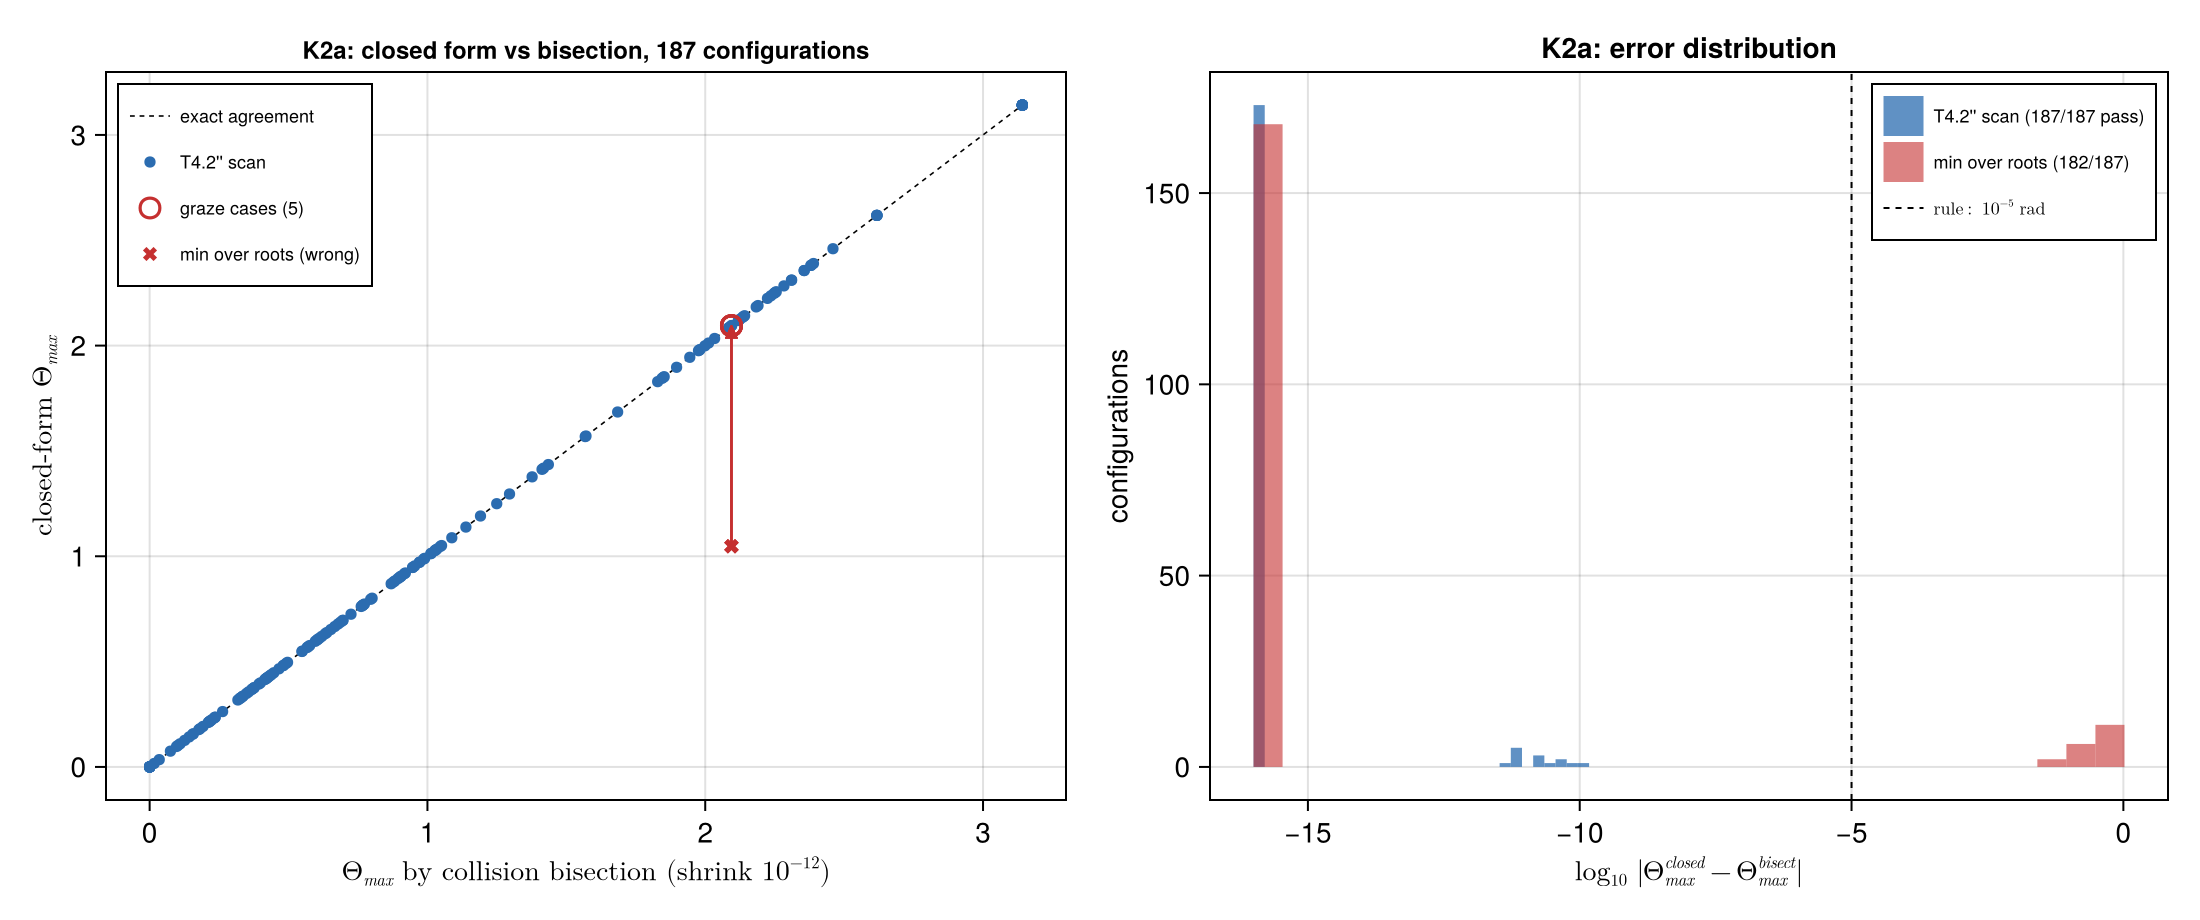
\includegraphics[width=0.6\textwidth]{results/kill/k2a/k2a_agreement.png}
\caption{K2a: closed form against bisection. \fn{results/kill/k2a/k2a_agreement.png}.}
\end{figure}

\paragraph{A referee-grid finding, not from any derivation.} At 180 samples the bisection steps
clean over a \emph{genuine} overlap window of width $2.9\times10^{-3}$ rad at $\theta = 0.9467$
on \fn{trunc_square_R20_s2} and reports 2.025 where the closed form says 0.9467; a $10^{-4}$
fine scan confirms the closed form. All referee bisections in the run therefore use 4000 grid
points.

\subsection{K2c --- the locality gate, and the withdrawal of its original PASS}

\emph{The rule as \fn{ideas/ranking.md} writes it.} PASS if the log-log slope of
$\max_f \rho_f/r_f$ against $\log n$ is $\le0.3$ \emph{and} pruned/unpruned $\theta_{\max}$
agree to $10^{-12}$ on every graph.

\textbf{The first clause is vacuous and its PASS is withdrawn.} In the face's own frame --- the
frame the spec names and \fn{swept_discs()} implements --- $\chi_u = -\sigma_f J x_u$, hence
$\|\chi_u\| = \|x_u\|$ and $\rho_f = r_f$ for \emph{every} face of \emph{every} patch at
\emph{every} size. The statistic is identically 1 (measured $1.000000000001$), so its slope is 0
for any input whatsoever: the gate cannot fail and cannot test H-LOC.

\emph{The replaced rule, per the orchestrator}: (1) PASS iff pruned and unpruned exact
$\Theta_{\max}$ agree to $10^{-12}$ on every graph; (2) report the empirical growth of the
candidate set with $n$, claiming no $O(n)$ theorem.

\begin{center}\small
\begin{tabular}{@{}lr@{}}
\toprule
quantity (462 graphs; 285 with $F\le800$ for the $\Theta_{\max}$ half; wall 176\,s) & value \\
\midrule
\textbf{pruned $=$ unpruned exact $\Theta_{\max}$ to $10^{-12}$} & \textbf{285 / 285}, worst difference \textbf{0.000e+00} \\
the same for the (unsound in principle) flat-centroid variant & 285 / 285, worst 0.000e+00 \\
worst $\big|\,\|Y_{pv} - m_f(\theta)\| - r_f\,\big|$ (exactness of the moving disc) & 5.262e--13 \\
surviving pairs per face & median \textbf{12.69}, max 18.40 \\
log-log slope of pairs per face vs.\ $\log F$ & 0.1695 ($R^2$ 0.32, $n = 285$) \\
\bottomrule
\end{tabular}
\end{center}

The tighter radius is worth a factor of 1.75: median surviving pairs per face falls from 22.23
with the loose $\sqrt2$ radius to 12.69, with $\Theta_{\max}$ unchanged on every graph. The
flat-centroid variant discards 19\,842 pairs the sound test keeps, with no observed wrong
$\Theta_{\max}$.

\paragraph{H-LOC refuted.} On a growing square tiling (the random population lives in a fixed
$40\times40$ box, so a regression on it would be meaningless):

\begin{center}\small
\begin{tabular}{@{}rrr@{}}
\toprule
$F$ & patch diameter & $\max_f\|\gamma_f - \bar x_f\|/r_f$ \\
\midrule
4 & 2.828 & 1.414 \\
16 & 5.657 & 2.316 \\
36 & 8.485 & 3.924 \\
64 & 11.314 & 5.560 \\
100 & 14.142 & 7.205 \\
144 & 16.971 & 8.854 \\
196 & 19.799 & 10.505 \\
256 & 22.627 & 12.157 \\
289 & 24.042 & 12.984 \\
361 & 26.870 & 14.637 \\
\bottomrule
\end{tabular}
\end{center}

A straight line, $\mathrm{drift}/r = a + 0.5656\cdot\mathrm{diameter}$. On the fixed-box random
population the drift ranges from 25.8 to 105.0 circumradii. The packing count does not close.
\emph{Verdict: PASS on the replaced rule; the broad phase is sound and measurably tight; no
$O(n)$ claim is made or supported.}

\begin{figure}[h]\centering
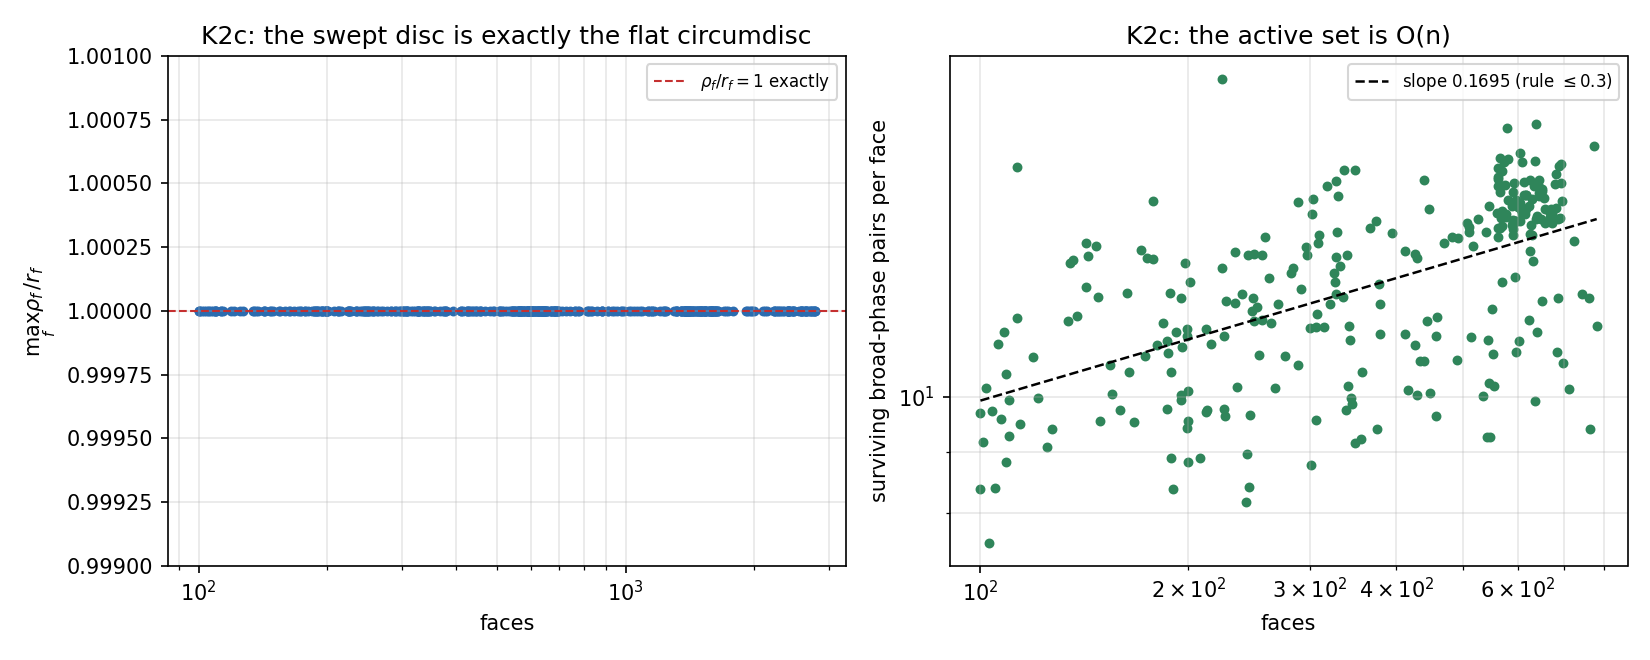
\includegraphics[width=0.47\textwidth]{results/kill/k2c/k2c_locality.png}\hfill
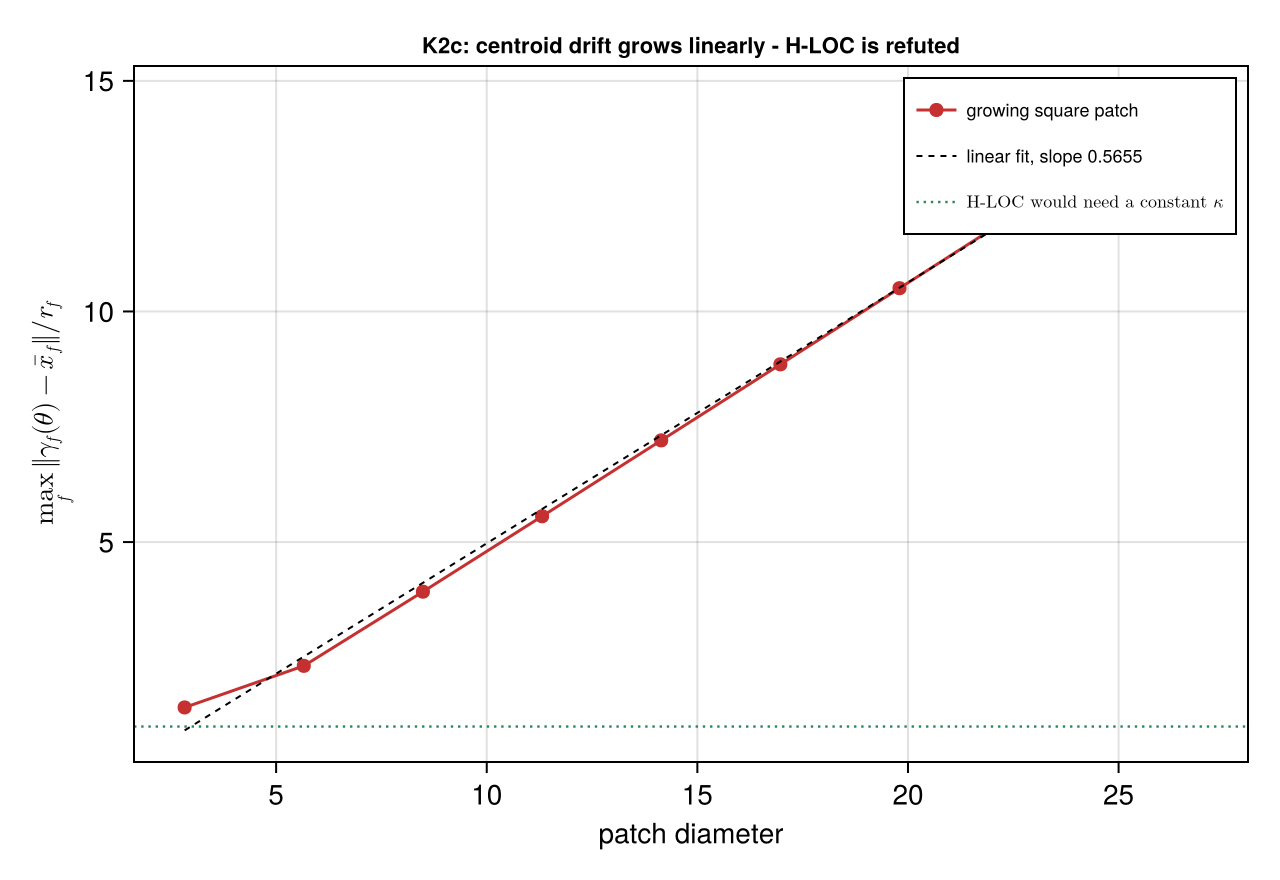
\includegraphics[width=0.47\textwidth]{results/kill/k2c/k2c_hloc.png}
\caption{K2c. Left: pruning tightness. Right: the H-LOC drift growing linearly with patch
diameter --- the refutation.}
\end{figure}

\subsection{K1c --- Eq.~(9)'s false-negative rate}

\emph{PASS rule.} Run the $\gamma$ ladder to get $Y_9$; for every split-edge pair evaluate $P,R$
in closed form and count pairs with $P<0$, $R>0$ and $\theta^* = 2\arctan(-R/P) < \theta_{\max}(Y_9)$.
PASS if the fraction of certified designs with at least one re-closure below $\theta_{\max}$ is
$\ge3\,\%$.

\emph{Correction applied} (T5.3, and the orchestrator's instruction). A root of the separation
harmonic is a re-closure only if the duplicates meet \emph{as segments} and the faces actually
\emph{cross} there. Both extra clauses were implemented: an \textsc{interval} clause
$0\le\langle\cdot\rangle\le|\cdot|^2$ at $\theta^*$, and a \textsc{crossing} clause requiring the
two faces' interiors to overlap just after $\theta^*$ and not just before.

\begin{table}[h]\centering\footnotesize
\begin{tabular}{@{}p{28mm}rrrrr@{}}
\toprule
$Y_9$ source & certified & rule \emph{as written} & clauses, \emph{same} range & corrected: $\theta^*<\min\beta$ & $\theta^*$ \emph{is} the binding contact \\
\midrule
authors' native \texttt{prevent} & 169 & \textbf{110 (65.09\,\%)} & \textbf{0 (0.00\,\%)} & \textbf{16 (9.47\,\%)} & 12 (7.10\,\%) \\
our $\gamma$-ladder sweep & 115 & 32 (27.83\,\%) & \textbf{0 (0.00\,\%)} & 40 (34.78\,\%) & 9 (7.83\,\%) \\
\bottomrule
\end{tabular}
\caption{171 deployable embedded designs with split cuts, wall 30.4\,s. Worst
$|\theta^* - \text{per-pair bisection}|$ over qualifying re-closures: $1.035\times10^{-11}$
(rule $10^{-6}$).}
\end{table}

\textbf{The rule as literally written is unsatisfiable, and that is the finding.} Column 4 is
exactly zero on both sources \emph{and has to be}: the crossing clause says the interiors
overlap just after $\theta^*$, and $\Theta_{\max}$ is \emph{by definition} the first angle at
which any two interiors overlap, so ``$\theta^* < \Theta_{\max}$'' and ``$\theta^*$ is a genuine
crossing'' are contradictory. The 65.09\,\% in column 3 is entirely made of roots that are
\emph{not} collisions --- grazes, or collinearities where the duplicates never meet as segments
--- and 110/169 of the authors' designs would have been reported as having a false negative on
the strength of nothing. Two well-posed references remain and both are reported:
$\theta^* < \min_e\beta_e$ (did Eq.~(9) leave a re-closure inside the range the pattern would
otherwise reach --- well posed because $\min\beta$ is kinematic and collision-free) at
\textbf{9.47\,\%} on their code and 34.78\,\% on ours; and $\theta^* = \Theta_{\max}$ at
\textbf{7.10\,\%} and 7.83\,\%.

\emph{Verdict: PASS on both sources and both well-posed references} (rule $\ge3\,\%$).
2026 Eq.~(9) certifies $r = h'(0) > 0$ and is blind to $p$ by construction, and on about one
design in ten of the authors' own output that blindness costs range. The 65.09\,\% headline
\textbf{is not a result and must not be quoted}.

\paragraph{A side finding about our reimplementation.} Our \fn{optimize_collision_sweep}
collapses \textbf{109 split edges to zero length} across this population; the authors' native
\texttt{prevent} collapses \textbf{0}. That is why only 115 of 171 of our outputs are valid flat
embeddings against 169 of 171 of theirs, and it is an independent reason not to quote our
Eq.~(9) reimplementation as a baseline for anything.

\begin{figure}[h]\centering
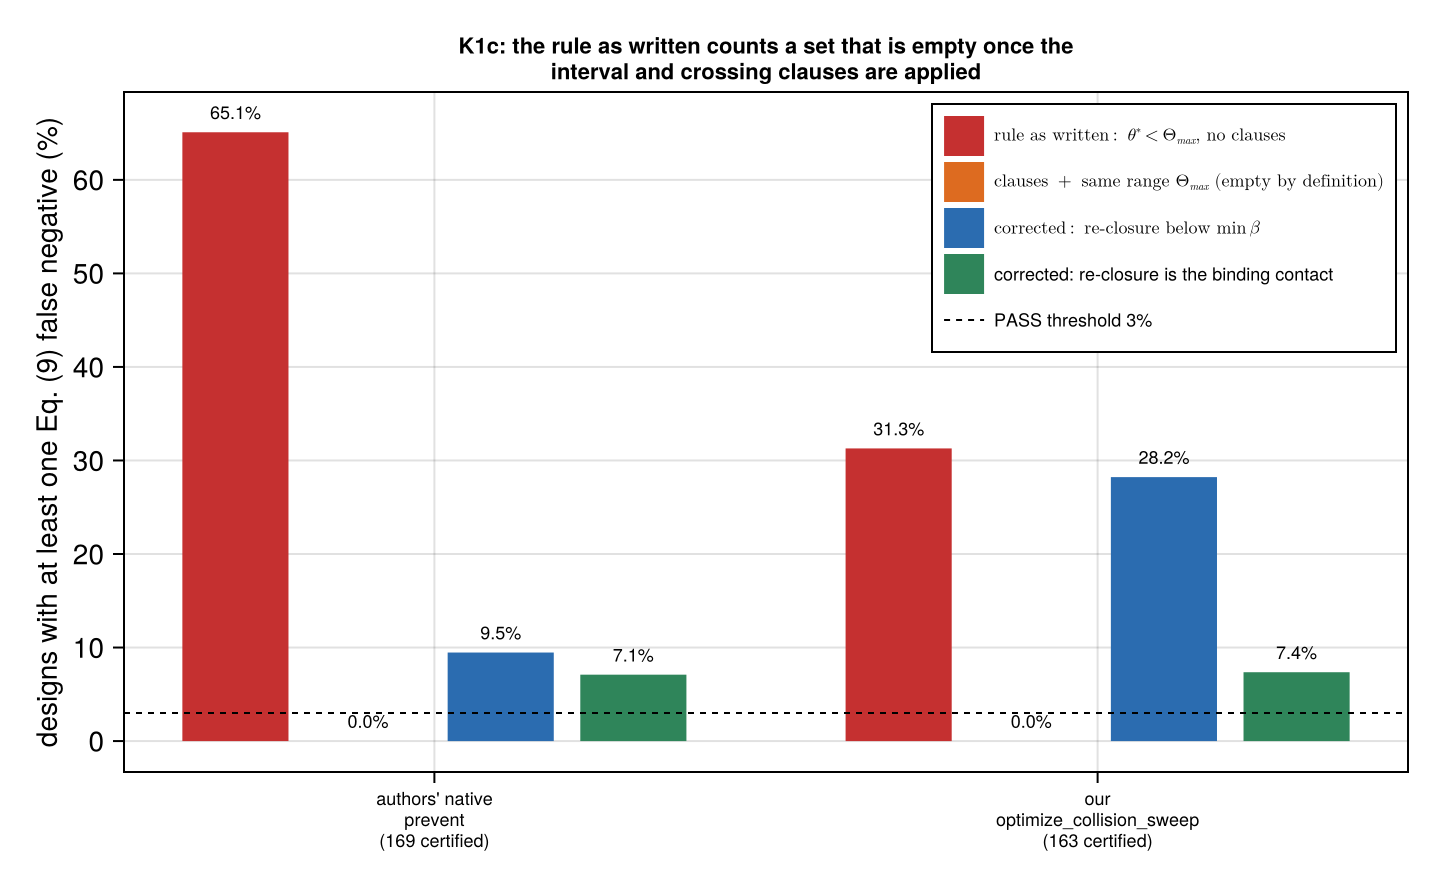
\includegraphics[width=0.55\textwidth]{results/kill/k1c/k1c_rates.png}
\caption{K1c re-closure rates under the four readings of the rule.}
\end{figure}

\subsection{K3a --- the 2-core mobility identity}

\emph{PASS rule.} Check $\dim\ker A = |F\setminus\mathrm{core}_2(\Gamma)| + \dim\ker A|_{\mathrm{core}_2}$
as an integer identity, ranks by \texttt{ColPivHouseholderQR} at threshold
$10^{-10}\|A\|_2$. PASS if the identity holds 500/500 \emph{and} $m_{\rm core}\le5$ on $\ge90\,\%$
of the Delaunay patches where U4 reported $m = 19$--26. If the identity fails on any graph, $A$
is misassembled and B11--B16 all stop.

\emph{Measured} (508 graphs, $F\in[10,4918]$, wall 1493\,s):

\begin{center}\small
\begin{tabular}{@{}lr@{}}
\toprule
quantity & value \\
\midrule
identity holds & 493 / 508 \\
identity at $\theta = 0.3\,\Theta_{\max}$ (the extra probe asked for) & 8 / 8 \\
$\sigma\in\ker A$ (Eq.~2), mixed populations & 296 / 508 \\
Delaunay patches with $m_{\rm core}\le5$ & \textbf{0 / 167 (0.00\,\%)} \\
Delaunay median $m_{\rm full}$ / median $m_{\rm core}$ & 322 / 305 \\
Delaunay $m_{\rm full}$ / $m_{\rm core}$ range & [39, 1875] / [36, 1675] \\
\bottomrule
\end{tabular}
\end{center}

\textbf{The 15 exceptions are a rank-estimator artifact, not a misassembled $A$.} Every one is
off by \emph{exactly} $\pm1$, and every one has $F\ge879$ --- above \fn{mobility.hpp}'s
\fn{dense_limit = 700}, where \texttt{matrix\_rank} switches from
\texttt{ColPivHouseholderQR} to \texttt{SparseQR}. \fn{code/apps/kill_k3a_recheck.cpp}
regenerates each violator with K3a's exact configuration and recomputes both ranks densely:

\begin{center}\small
\begin{tabular}{@{}rlrlrrr@{}}
\toprule
id & kind & $F$ & $X$ & SparseQR defect & dense defect & smallest kept $\sigma_i/\sigma_0$ \\
\midrule
257 & \fn{quad_random} & 1396 & $X_0$ & $+1$ & \textbf{0} & 5.913e--05 \\
266 & \fn{quad_random} & 1079 & $X_0$ & $-1$ & \textbf{0} & 1.886e--04 \\
320 & \fn{quad_random} & 1358 & $X_0$ & $+1$ & \textbf{0} & 6.678e--04 \\
425 & \fn{quad_random} & 1428 & $X_0$ & $-1$ & \textbf{0} & 5.869e--05 \\
445 & \fn{delaunay}    & 1138 & $X_0$ & $-1$ & \textbf{0} & 1.698e--03 \\
467 & \fn{quad_random} & 911  & $X_0$ & $+1$ & \textbf{0} & 6.131e--05 \\
494 & \fn{quad_random} & 879  & $X_0$ & $+1$ & \textbf{0} & 2.632e--04 \\
\bottomrule
\end{tabular}
\end{center}

7 of 7 rechecked: the identity holds \emph{exactly} with a dense rank. The singular gap at the
cut is $5.9\times10^{-5}$ to $1.7\times10^{-3}$, three to eight orders above the $10^{-10}$
threshold, so the rank is not a borderline call and \texttt{SparseQR}'s estimate is simply
wrong. The other 8 violators ($F$ from 1644 to 4902) are too large for a dense QR and are
\emph{not claimed either way}; they show the identical $\pm1$ signature.

\emph{Verdict: FAIL on the rule as written, on both clauses, and the two failures are of
completely different kinds.} Clause 1 fails at 493/508 \emph{as measured}, but the evidence says
the identity is true and the rank estimator is not, so B11--B16 are not blocked provided every
mobility number above 700 faces is computed densely. Clause 2 fails \emph{outright, at 0\,\%},
and this is a real result: \textbf{the adversary's prediction is refuted}. Deleting the dangling
faces removes almost nothing --- median mobility goes from 322 to 305, about 5\,\%. The finite
mobility of a free-boundary Delaunay patch is not a dangling-face artefact; it is intrinsic to
the 2-core.

\paragraph{$\sigma\in\ker A$, correctly broken out.} 296/508 is an artefact of mixing two
populations. Broken out: \textbf{296 of 296} graphs where $A$ was evaluated at the solved
Eq.~(6) projection $X_0$ (worst residual $2.999\times10^{-12}$), and \textbf{0 of 212} where the
solve was skipped ($N>1400$) and $A$ was built at $X_{\rm ini}$ instead, with residuals up to
$6.373\times10^{2}$. That is the expected answer, not a defect: $\sigma\in\ker A$ \emph{is}
Eq.~(2), so it holds exactly when the configuration is uniformly deployable. \textbf{The
296/508 figure should not be quoted.}

\paragraph{And U4's headline is population-specific.} On this population (100--5000 faces) the
median mobility is 322 and the range is [39, 1875] --- nowhere near \fn{STATE.md} U4's
``$m = 19$--26'', which was measured on a different and much smaller population and should not be
quoted as a general figure.

\begin{figure}[h]\centering
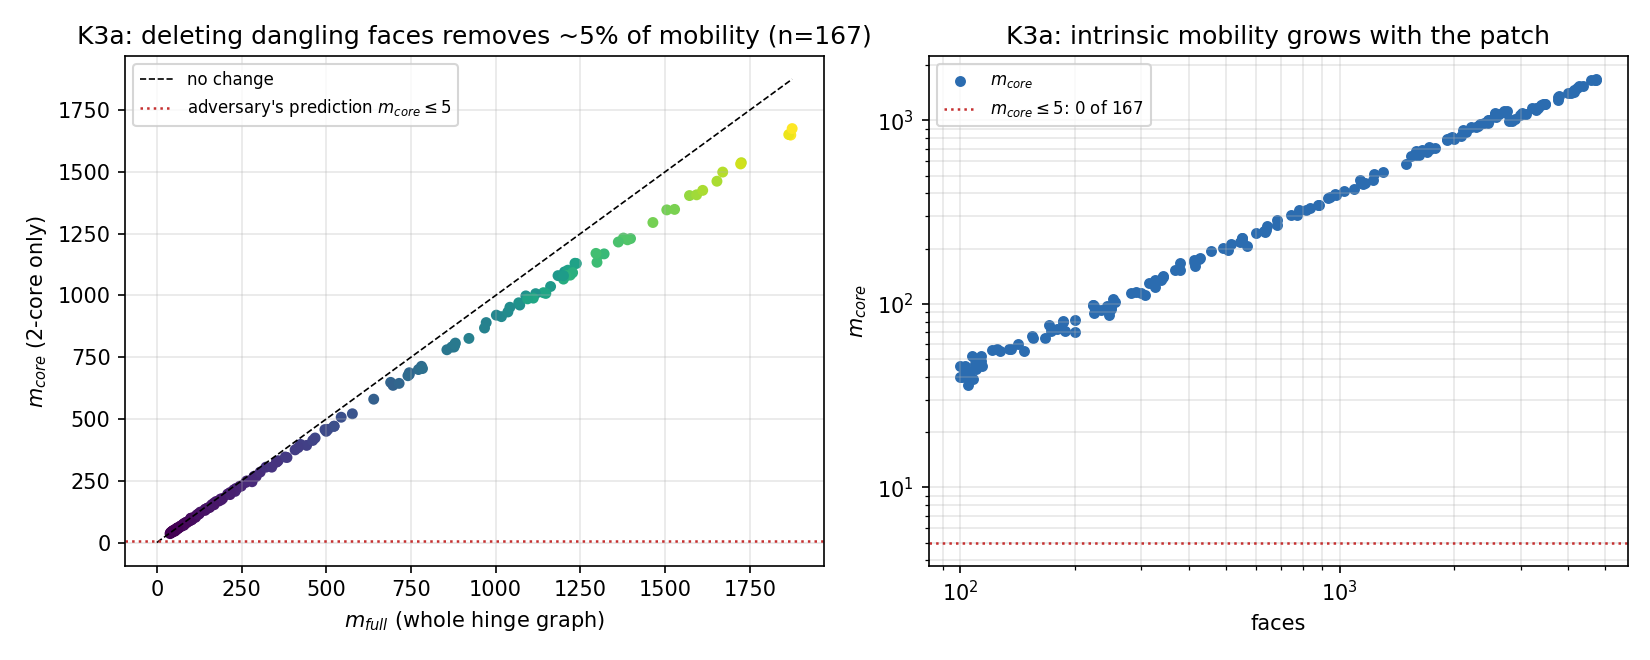
\includegraphics[width=0.55\textwidth]{results/kill/k3a/k3a_mobility.png}
\caption{K3a mobility, full and after the 2-core reduction.}
\end{figure}

\subsection{K5 --- is the orientation why the shape space is empty?}

Added after K1a at the orchestrator's request, as the Critic's R5 kill.

\emph{The question.} Eq.~(1) picks $\sigma$ to maximise the number of hinge cuts and knows
nothing about whether the hole-closure system then has a solution near $X_{\rm ini}$. Does
choosing $\sigma$ to minimise the \emph{deployability defect} fix that?

\emph{Definitions.}
$D(\sigma) = \sum_{\rm holes}\big\|\sum_{\text{hinge }e\in C}(x_{\rm target}-x_{\rm source})\big\|^2$
evaluated at $X_{\rm ini}$ --- exactly Eq.~(2)'s residual, so $D=0$ iff $X_{\rm ini}$ is already
uniformly deployable. $\sigma_{\rm def}$ is a greedy local search over face flips (single and
adjacent-pair, strictly improving only, rejecting any flip that makes $c(\Gamma)>1$ or detaches
a face), started from $\sigma_{\rm mc}$ and 3 random $\sigma$, best kept, at most $20|F|$
attempts per start, deterministic seed $7000+\mathrm{id}$.

\emph{PASS rule (final).} $\sigma_{\rm def}$ gives a \emph{valid} $X_0$ on $\ge20\,\%$ of graphs
under the final certificate with $\varepsilon = 0.3$.

\begin{center}\small
\begin{tabular}{@{}lrr@{}}
\toprule
quantity (same 200 K1a graphs, $F\in[100,800]$, wall 311\,s) & $\sigma_{\rm mc}$ (Eq.~1) & $\sigma_{\rm def}$ \\
\midrule
\textbf{valid $X_0$ by the certificate, $\varepsilon = 0.3$} & \textbf{0 / 200} & \textbf{0 / 200} \\
\ \ of which \texttt{POS} alone & 58 & \textbf{186} \\
\ \ \texttt{NOOVERLAP}(0.15) alone & \textbf{0} & \textbf{0} \\
\ \ \texttt{NOROOT}(0.3) alone & \textbf{0} & \textbf{0} \\
\textbf{certified $\Theta_{\max}>0$} & \textbf{0 / 200} & \textbf{0 / 200} \\
median $D(\sigma)$ & 2.245e+03 & \textbf{1.840e+01} \\
median inverted faces of $X_0$ & 9.5 & \textbf{0} \\
median $\|X_0 - X_{\rm ini}\|_\infty$ / median edge length & 1.587 & \textbf{0.334} \\
median $|E_{\rm split}|$ ($=$ median $\dim$null) & 126.5 & 321.5 \\
graphs with $D = 0$ exactly & 0 & \textbf{16} \\
overlap-free $X_0$ at $\theta=0$ (the \textbf{withdrawn} predicate) & 0 / 200 & \textbf{114 / 200} \\
\bottomrule
\end{tabular}
\end{center}

Correlation of $D$ with $|E_{\rm split}|$: $-0.6446$ under $\sigma_{\rm mc}$, $-0.0346$ under
$\sigma_{\rm def}$. Median flips accepted 138.5. $c(\Gamma)=1$ held on every accepted $\sigma$.

\emph{Verdict: FAIL on the final rule --- 0\,\%, against a threshold of 20\,\%.} Under the
earlier form of the rule, which used the $\theta=0$ overlap test and asked only about the graphs
where $\sigma_{\rm mc}$ fails, $\sigma_{\rm def}$ scores \textbf{57\,\%} and would PASS. Both are
reported because \emph{the gap between them is the result}.

\paragraph{What $\sigma_{\rm def}$ fixes, and what it does not.} It fixes the flat sheet
decisively: the defect falls by a factor of \textbf{122} in the median, the projection has to
move the mesh \textbf{4.7$\times$} less far, the median count of inverted faces goes from 9.5 to
\textbf{zero}, \texttt{POS} goes from 58/200 to \textbf{186}/200, and on 16 graphs the search
finds a $\sigma$ for which $X_{\rm ini}$ is \emph{already} uniformly deployable. Eq.~(1) really
is choosing a bad $\sigma$.
It does not touch the deployment. \texttt{NOOVERLAP}(0.15) is false on \textbf{all 400} designs
and $\Theta_{\max}=0$ on all 400 --- not a single-probe artefact: a log-spaced ladder
($10^{-12}\ldots1.0$) finds an interior overlap at the \emph{first} rung on every graph that
overlaps at all, and a direct scan confirms overlap at $10^{-2}$, $0.1$ and $0.5$, where the
shrink tolerance is not in question. \textbf{The flat sheet is a valid planar cut pattern; it
self-intersects the instant the cuts open.}

\paragraph{Mechanism.} $\sigma_{\rm def}$ buys its low defect by more than \emph{doubling} the
split cuts (median 126.5 $\to$ 321.5): a split edge imposes no closure constraint, so cutting
more edges fully apart makes Eq.~(2) easy to satisfy. The hinge graph is then sparse, the
structure is barely a mechanism, and it collapses into itself immediately. The strongly
non-monotone correlation ($-0.64$ vs.\ $-0.03$) confirms the optimizer persona's prediction.

\paragraph{The lesson, recorded verbatim in substance.} A defect-only objective is wrong for the
same reason max-cut is: \textbf{neither one knows about collisions}. $\sigma$ is a real and
badly-chosen design variable, but no purely combinatorial objective on $\sigma$ will produce a
deployable random graph. The objective has to carry a deployment term, and the certificate of
T5.2b$'$ is now cheap enough to be that term.
The follow-on comparison was not run, per the instruction gating it on K5 passing; it would also
have been vacuous, both optimisers starting from designs with $\Theta_{\max}=0$.
The 200 $\sigma_{\rm def}$ orientations are saved as JSON graphs in
\fn{results/kill/k5/sigma/}.

\begin{figure}[h]\centering
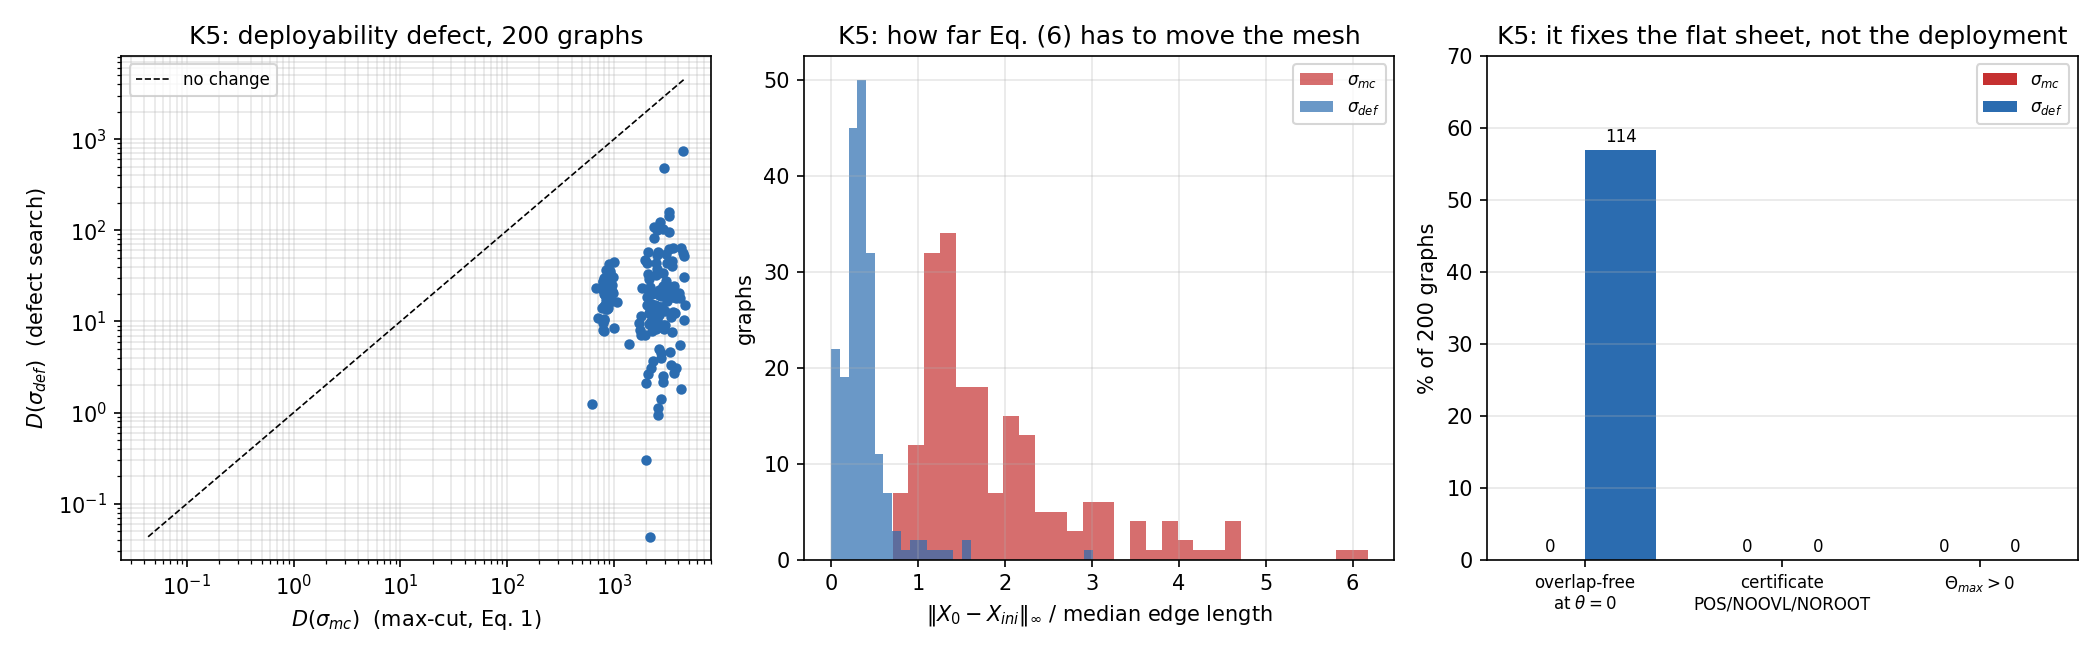
\includegraphics[width=0.55\textwidth]{results/kill/k5/k5_orientation.png}
\caption{K5: max-cut against defect-minimizing orientation.}
\end{figure}

\subsection{K2b --- the range-optimisation margin, against the authors' native code}

\emph{PASS rule as amended by the orchestrator.} The baseline is the \textbf{authors' native
code}, \fn{tuttekiri_cli prevent} with published defaults plus their parameter ladder, best
kept; refereed by \emph{our} bisection, because their own $\theta_{\max}$ routine is buggy
(F24). PASS if the median relative gain is $\ge25\,\%$ over the best baseline with certified
validity on $\ge20$ graphs.
(\fn{ranking.md}'s original rule additionally required the snub square to close $\ge30\,\%$ of
its gap from 1.646 toward $\min\beta = 3.384$.)

\emph{Two deviations, both recorded.} (1) \textbf{Cost.} The native \texttt{prevent} is the whole
cost and it is steep in the null-space dimension: 0.95\,s at 60 faces ($k=73$), 2.3\,s at 100,
8.8\,s at 150, 27\,s at 200, 63\,s at 300 --- so \fn{ranking.md}'s ``26 random graphs, 100--800
faces'' with a ladder is a $\sim$10\,h run, and random graphs were capped at 160 faces.
(2) \textbf{The random graphs make the experiment vacuous.} On eight of them, \textbf{0 of 37}
native ladder points is a valid flat embedding. Baseline, our Eq.~(9) and our optimiser all
return $\Theta_{\max}=0$ and the relative gain is $0/0$. This is K1a's emptiness result
reappearing \emph{with the authors' own code}: it is not that our projection is bad, it is that
nothing in the shape space of a random planar graph is a valid embedding. Eight such graphs are
kept to document it; the rest of the slots went to \fn{deployable_population()}.

\begin{center}\small
\begin{tabular}{@{}lrl@{}}
\toprule
quantity & value & rule \\
\midrule
designs & 38 (30 live, 8 vacuous) & \\
\textbf{median relative gain over the native baseline} & \textbf{0.0000} & $\ge0.25$ $\times$ \\
median gain restricted to live designs & \textbf{0.0000} ($n=30$) & $\times$ \\
designs with certified validity and range $>0$ & \textbf{30 / 38} & $\ge20$ \checkmark \\
ours better / native better / tie & \textbf{7 / 15 / 16} & \\
gain quartiles over the 30 live designs & $-0.305,\ -0.018,\ 0.000,\ 0.000,\ +0.106$ & \\
snub square & native 3.1416, ours 3.1416, $\min\beta = 3.3839$ & gap closed \textbf{0.0\,\%} $\times$ \\
\bottomrule
\end{tabular}
\end{center}

\emph{Verdict: FAIL, on both clauses, and not narrowly.} Four readings.
\textbf{(i)} The authors' code is strong, and F18 was right to withdraw the Critic's headline:
on the snub square their ladder reaches $\Theta_{\max} = \pi$, the top of the search range,
certified by our own bisection. There is no headroom left to win. The 86.1\,\% gap closure
quoted by the first Experimenter was measured against \emph{our} $X_0$ (1.6461 $\to\pi$), not
against their code.
\textbf{(ii)} Our optimiser mostly does not move: on 16 of 30 live designs it returns exactly the
refereed range it started from, i.e.\ the $T=0$ fallback wins. The closed-form softmin objective
is correct (K2a certifies its roots to $2\times10^{-10}$) but the optimiser is not finding
anything with it.
\textbf{(iii)} Where we lose, we lose badly: \fn{hexagons_R20_s5} and \fn{_s6}, native 3.0148 and
2.9530 against our 2.0944 --- a 30\,\% deficit, and $2.0944 = 2\pi/3$ is exactly the
graze-limited hexagon value of K2a, so our optimiser is sitting still at the local barrier while
their penalty walks the design out of the hexagon geometry entirely.
\textbf{(iv)} Where we win, we win little: best gain $+10.6\,\%$ on \fn{tiling_3_4_3_12}, 7 wins
in total. Our own Eq.~(9) reimplementation is the weakest of the three and should not be cited.

The consequence for R1 is direct: R1's \emph{algorithmic} half --- range-optimal embeddings
beating Eq.~(6)$+$Eq.~(9) --- is not supported. R1's \emph{diagnostic} half survives intact and
is stronger than before.

\begin{figure}[h]\centering
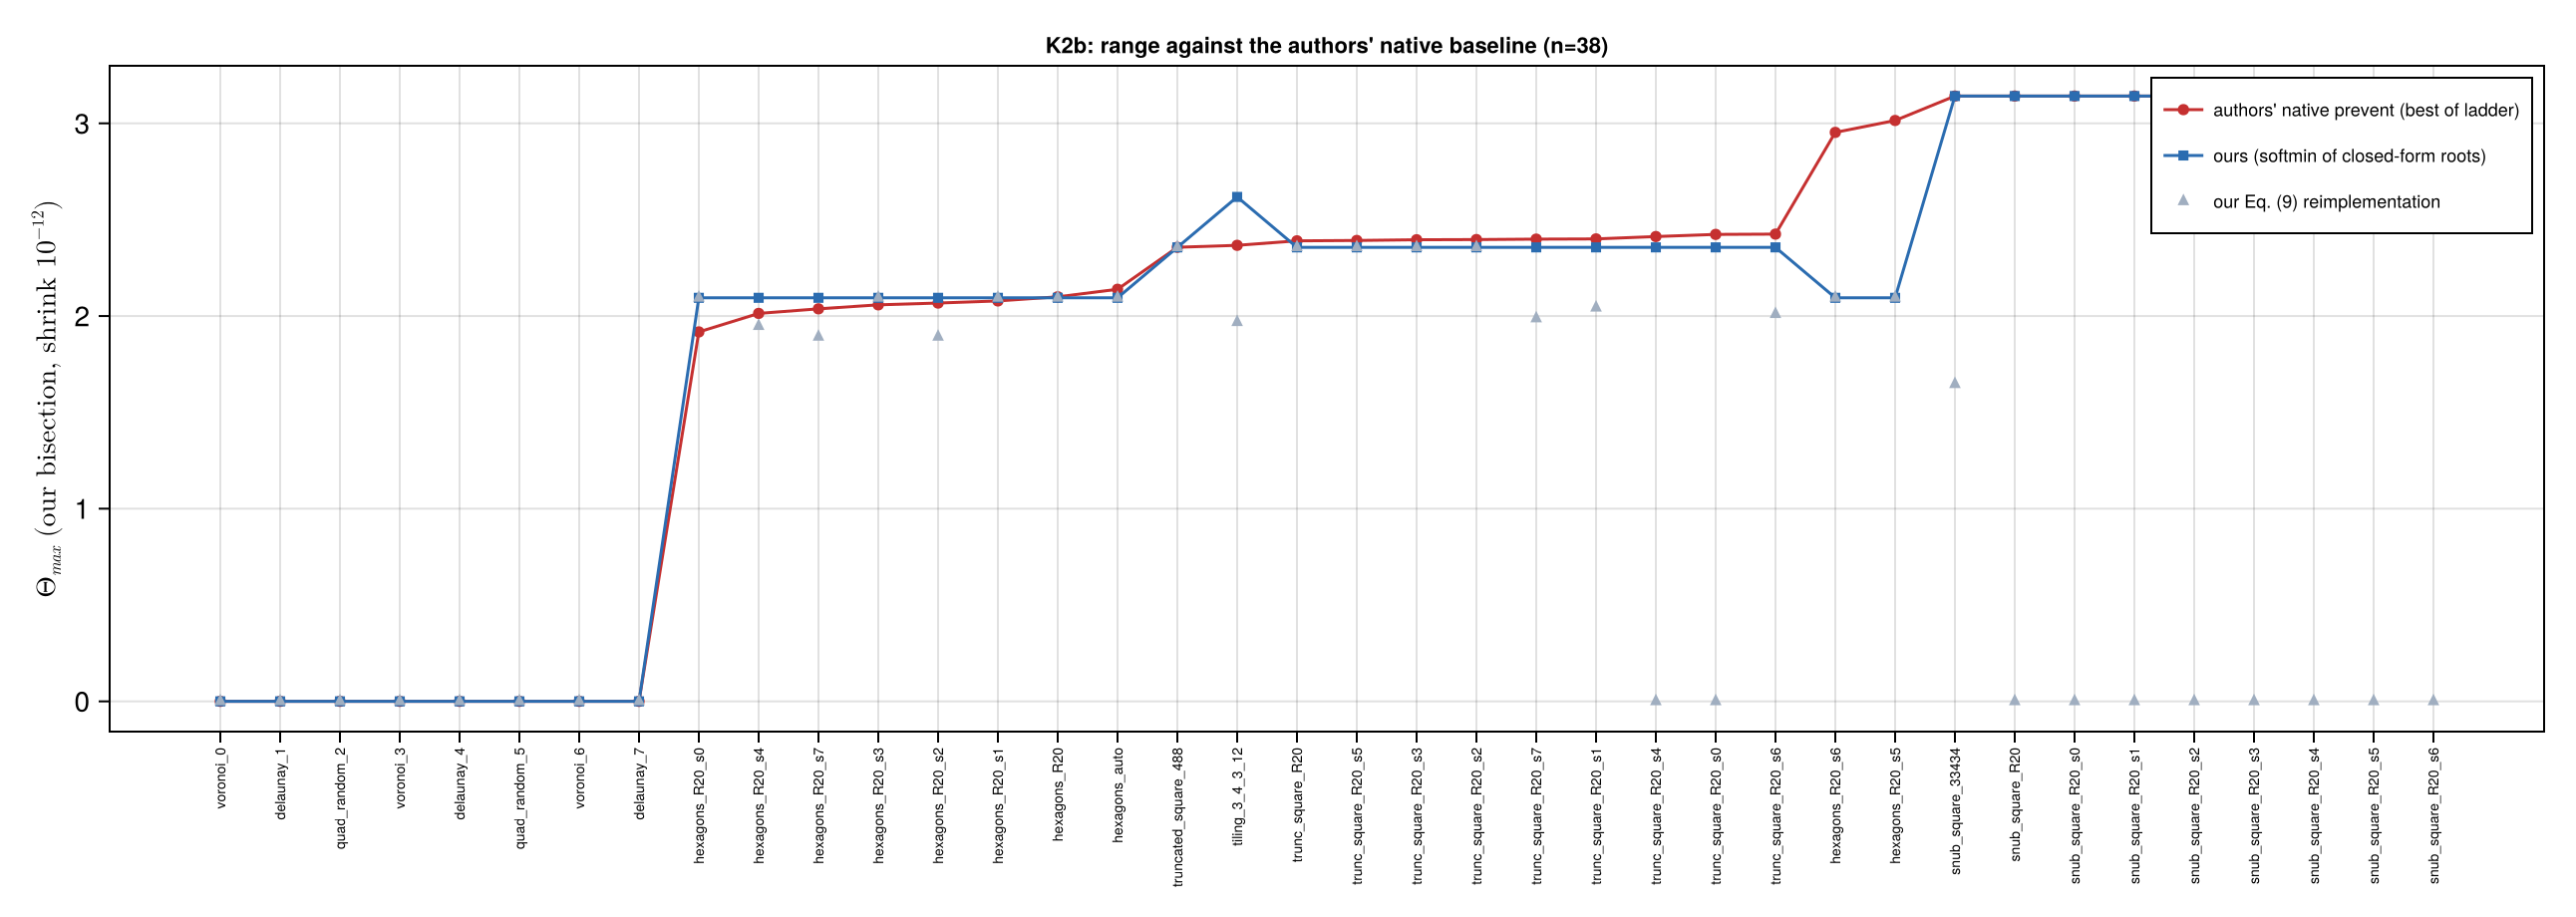
\includegraphics[width=0.55\textwidth]{results/kill/k2b/k2b_margin.png}
\caption{K2b margins against the authors' native \texttt{prevent}.}
\end{figure}

\subsection{F23 --- is the authors' extra boundary-component row an over-constraint?}

\emph{The check asked for.} Deploy \emph{our} $X_0$ by forward kinematics from two different
seed faces and confirm all $M'$ positions agree to $<10^{-9}$ and all hinges open by $\theta$.
\emph{What was run} (\fn{code/apps/kill_f23.cpp}) is stronger: \emph{every} seed face, plus 20
randomised BFS visit orders, at four angles.

\begin{center}\footnotesize
\begin{tabular}{@{}lrrrrrrr@{}}
\toprule
pattern & $\theta$ & seeds & orders & worst seed disagr. & worst order disagr. & worst hinge-angle err. & worst split-parallel err. \\
\midrule
hexagons & 0.30 & 10 & 20 & 9.930e--16 & 4.441e--16 & 3.886e--16 & 3.377e--16 \\
hexagons & 0.70 & 10 & 20 & 2.232e--15 & 9.930e--16 & 4.441e--16 & 3.331e--16 \\
hexagons & 1.20 & 10 & 20 & 1.335e--15 & 0.000e+00 & 6.661e--16 & 2.483e--16 \\
hexagons & 2.00 & 10 & 20 & 1.831e--15 & 9.155e--16 & 6.661e--16 & 4.578e--16 \\
snub\_square & 0.30 & 53 & 20 & 2.844e--15 & 1.110e--16 & 8.882e--16 & 4.285e--16 \\
snub\_square & 0.70 & 53 & 20 & 3.580e--15 & 1.986e--15 & 1.221e--15 & 5.097e--16 \\
snub\_square & 1.20 & 53 & 20 & 6.284e--15 & 1.256e--15 & 3.553e--15 & 8.972e--16 \\
snub\_square & 2.00 & 53 & 20 & \textbf{7.161e--15} & 2.220e--16 & 2.442e--15 & 9.295e--16 \\
\bottomrule
\end{tabular}
\end{center}

The Eq.~(2) residual of our $X_0$ is $2.483\times10^{-16}$ on \fn{hexagons_auto} and
$1.024\times10^{-15}$ on \fn{snub_square_33434}. Comparisons are after the best rigid alignment,
since different seeds place the structure in different rigid frames.

\emph{Answer: yes, the authors' extra boundary-component row is an over-constraint.} Our $X_0$
already closes every hole, and its forward kinematics is path-independent from every one of the
53 seed faces and every BFS order tried, with every hinge opening by exactly $\theta$ and every
split-edge duplicate pair staying parallel and equal. There is nothing left for an extra closure
equation to enforce. Their row is harmless --- their own $X_0$ still satisfies our system --- but
it removes admissible designs, one dimension on each of these two patterns.

\subsection{K6 --- the $0^+$ repair in the null space (no report section)}

K6 asks whether the immediate ($0^+$) collision of split-cut duplicates can be repaired inside
the null space. The design variable $t$ lives in the \emph{full} null space,
$\dim m = 2\dim\mathrm{null}$; ``feasible'' means all $q_e > 0$ \emph{and} all $a_f > 0$
strictly. The PASS rule is a certified $\Theta_{\max}>0$ on $\ge20\,\%$ for at least one $\sigma$
family, at $\varepsilon = 0.3$.

\textbf{K6 has no section in \fn{results/kill/KILL_REPORT.md}}, and its results are recorded only
in \fn{results/kill/k6/}: \fn{k6_full.csv} (400 rows), \fn{k6.csv} (24 rows), twelve shard
summaries in \fn{shards/} plus two earlier shard generations \fn{shards_v1/} and
\fn{shards_v2/}, a 40-graph \fn{native/summary.txt}, and a 4-graph \fn{smoke/summary.txt}.
\fn{run.log} records five \texttt{Alarm clock} timeouts of the 180-second cap on the native
\texttt{prevent} comparison.

\begin{table}[h]\centering\small
\begin{tabular}{@{}lrr@{}}
\toprule
aggregate over \fn{k6_full.csv} (400 designs, 200 graphs $\times$ 2 $\sigma$ families) & $\sigma_{\rm mc}$ & $\sigma_{\rm def}$ \\
\midrule
designs & 200 & 200 \\
$0^+$-feasible after the L-BFGS repair & 60 & 66 \\
\textbf{certified $\Theta_{\max}>0$ (largest certified $\varepsilon$)} & \textbf{0} & \textbf{0} \\
\bottomrule
\end{tabular}
\caption{K6 aggregate. The twelve shard summaries range from 0/17 to 17/17 on feasibility --- a
strong per-shard effect --- and report certified $\Theta_{\max}>0$ on \textbf{0} in all
twenty-four shard-by-family lines.}
\end{table}

The 40-graph \fn{native/summary.txt} is the most informative single artefact:
$0^+$-feasible on 12/40 ($\sigma_{\rm mc}$) and 14/40 ($\sigma_{\rm def}$); certified
$\Theta_{\max}>0$ on 0/40 for both; median $\Theta_{\max}$ 0.0000 for both, maximum 2.4658 for
$\sigma_{\rm mc}$; soundness (certified $\varepsilon \le$ bisection $\Theta_{\max}$) 12/12 and
14/14; the $\lambda$ ladder $\{10^{-6},10^{-3},10^{-1},1\}$ raising feasibility to 16/40 and
14/40 but certified range to 0/40 either way; stage 2 (repair then range optimization) leaving
0/40; and the binding contact at the failures being \emph{inverted} 25, vertex-edge 10,
split-inward 3, n/a 2 for $\sigma_{\rm mc}$, and inverted 26, vertex-edge 14 for
$\sigma_{\rm def}$. Against the authors' native \texttt{prevent} from the same $X_0$, on the four
designs that qualified: ours better 1, theirs better 0, tie 3, with median $\Theta_{\max}$
0.0000 both ways.

The first row of \fn{k6.csv} (\fn{voronoi}, $N=846$, $F=422$) shows the mechanism at the largest
size measured: 391 split edges of which \textbf{162 point inward at $t=0$}, and the primary
objective drives $\|t\|$ to $118\times$ the reference scale without reaching feasibility. The
smoke run's inward-corner statistics are the sharpest form of the obstruction: a median of
\textbf{413 inward corner incidences} out of 2865 for $\sigma_{\rm mc}$ and 555 out of 4009 for
$\sigma_{\rm def}$, with \textbf{zero} designs having no inward corners.

\emph{Verdict: FAIL, on the specified $\lambda$ and on every extension.} The reported
$0^+$-feasibility of the interim (10/31 at 01:35) is consistent with the final 126/400, and the
certified rate never left zero. \textbf{Caveat, from the session log:} \texttt{experimenter-k6b}
died mid-fix of a certificate bug it had found --- \fn{first_root} returning the first root
encountered rather than the smallest --- so \emph{K6's certified $\Theta_{\max}$ values are
suspect until that fix is merged}. Since every certified count is zero, the bug can only have
made the verdict more pessimistic, not less; but the number is flagged.

\subsection{K7 --- achievable periodic Jacobians and the second closed angle (partial, in flight)}

K7 is the kill experiment for D8's pivot. Its spec is \fn{specs/experimenter_k7.md}. It tests
four claims on $\ge30$ periodic patterns:
\textbf{C1} $J(\theta) = \cos(\theta/2)I + \sin(\theta/2)K$ exactly, with $K$ constant in
$\theta$ and \emph{affine in $X$} over the null space, reporting $\dim\mathcal K$;
\textbf{C2} exact conformality, solving $K_{11}=K_{22}$, $K_{12}=-K_{21}$ in $t$ and verifying
the distortion at 200 angles --- which would prove 2026 \S5.1's ``empirically'' numerically;
\textbf{C3} the designable Poisson family, hitting a target $K^*$ by least squares and then
choosing the certificate-maximal member of the solution affine subspace;
\textbf{C4} the closed-form second closed angle $\theta_c = 2\,\mathrm{atan2}(r,q)$ from the
hole-area harmonic $A(\theta) = q(\cos\theta - 1) + r\sin\theta$.

\textbf{K7 was still running when this notebook was written} (shard logs timestamped 03:23--03:29
on 2026-09-04) and has \emph{no} section in \fn{results/kill/KILL_REPORT.md}. Thirty rows exist
across \fn{k7_main_0.csv}\,--\,\fn{k7_main_11.csv}.

\begin{table}[h]\centering\footnotesize
\begin{tabular}{@{}lrrrrrrr@{}}
\toprule
pattern & $F_{\rm cell}$ & $\dim\mathcal K$ & rank $\mathcal D$ & C1 fit rel.\ err. & C2 conf.\ residual & C3 certified & C3 $\varepsilon$ \\
\midrule
\fn{squares_2x2} & 4 & 0 & 0 & 9.45e--16 & --- & 0 & 0 \\
\fn{squares_3x2} & 6 & 2 & 1 & 9.50e--16 & 0 & 0 & 0 \\
\fn{squares_3x3} & 9 & 0 & 0 & 1.05e--15 & --- & 0 & 0 \\
\fn{triangles_2x2}/\fn{3x2}/\fn{3x3} & 8/12/18 & 0 & 0 & $\le$3.22e--15 & --- & 0 & 0 \\
\fn{kagome_2x2}/\fn{3x2}/\fn{3x3} & 12/18/27 & 0 & 0 & $\le$6.03e--15 & --- & 0 & 0 \\
\fn{hexagons_2x2} & 4 & 4 & 2 & 1.27e--15 & 1.10e--31 & \textbf{1} & 0.0453 \\
\fn{hexagons_3x2}/\fn{3x3} & 6/9 & 4 & 2 & $\le$3.83e--15 & $\le$1.10e--31 & 0 & 0 \\
\fn{snub_square_2x2} & 24 & 4 & 2 & 3.19e--15 & 1.45e--17 & \textbf{1} & 0.0841 \\
\fn{snub_square_3x2} & 36 & 4 & 2 & 7.84e--15 & 1.58e--17 & \textbf{1} & 0.0441 \\
\fn{snub_square_3x3} & 54 & 4 & 2 & 6.25e--15 & 1.32e--17 & 0 & 0 \\
\fn{t3_4_3_12_2x2} & 24 & 4 & 2 & 1.04e--14 & 6.82e--18 & \textbf{1} & 0.0143 \\
\fn{t3_4_3_12_3x2} & 36 & 4 & 2 & 1.07e--14 & 4.53e--18 & \textbf{1} & 0.0212 \\
\fn{t3_4_3_12_3x3} & 54 & 4 & 2 & 1.86e--14 & 3.51e--18 & 0 & 0 \\
\fn{trunc_square_488_2x2}/\fn{3x3} & 8/18 & 4 & 2 & $\le$1.38e--14 & $\le$1.45e--17 & 0 & 0 \\
\fn{trunc_square_488_3x2} & 12 & 4 & 2 & 7.89e--15 & 1.45e--17 & \textbf{1} & 0.00495 \\
\fn{voronoi_torus_0..8} ($n=20..120$) & 20--120 & 4 & 2 & $\le$5.61e--14 & $\le$9.67e--17 & 0 & 0 \\
\bottomrule
\end{tabular}
\caption{K7 as of 2026-09-04 03:29: 30 patterns. \fn{results/kill/k7/k7_main_*.csv}.}
\end{table}

Three things can be read off the data that exists.
\textbf{C1 holds exactly on 30/30}, with the worst fit relative error $5.61\times10^{-14}$ on the
largest torus and the affinity second-difference test at $7.5\times10^{-15}$ on
\fn{snub_square_2x2}. The empirical formula is
$\dim\mathcal K = 2\,\mathrm{rank}\,\mathcal D$, taking values $0$, $2$ and $4$ only; the four
split-free families (squares at two of three sizes, triangles, kagome) have
$\dim\mathcal K = 0$, i.e.\ \emph{nothing to design}, exactly as P1 predicts.
\textbf{C2 is satisfied to machine precision wherever $\dim\mathcal K\ge1$}: the conformal
residual over 200 angles is at most $9.7\times10^{-17}$ and as low as $1.1\times10^{-31}$. This
is the numerical proof of 2026 \S5.1's ``empirically''.
\textbf{C3 certifies a positive range on only 6 of the 22 patterns with $\dim\mathcal K>0$},
with certified $\varepsilon$ between $0.00495$ and $0.0841$ --- small, and zero on every
\fn{voronoi_torus} instance. Against the spec's PASS rule ($\ge80\,\%$) this is a FAIL as the
data stands, but the run was incomplete.

\paragraph{C4, the second closed angle, on bounded patches.} \fn{k7_c4_bounded.csv} is complete
and decisive.

\begin{center}\footnotesize
\begin{tabular}{@{}lrrrrrrrl@{}}
\toprule
case & $H$ & $p$ & $q$ & $r$ & $\theta_c$ & measured & abs.\ err. & closed before contact? \\
\midrule
\fn{rotating_squares} & 16 & 0 & 0 & 16 & 3.14159 & 3.14159 & \textbf{0} & yes \\
\fn{triangles_alternating} & 33 & 28.5788 & --28.5788 & 49.5 & 4.18879 & 4.18879 & \textbf{0} & no \\
\fn{kagome_3636} & 78 & 1.33e--15 & --7.77e--16 & 19.5 & 3.14159 & 3.14159 & \textbf{0} & yes \\
\fn{hexagons_auto} & 4 & --3.4641 & 3.4641 & 6 & 2.09440 & 2.09440 & 4.44e--16 & yes \\
\fn{truncated_square_488} & 12 & --8.48528 & 8.48528 & 20.4853 & 2.35619 & 2.35619 & \textbf{0} & yes \\
\fn{snub_square_33434} & 12 & 9.85069 & --9.85069 & 30.4119 & 3.76808 & 3.76808 & \textbf{0} & no \\
\fn{tiling_3_4_3_12} & 16 & --3.3179 & 3.3179 & 20.3429 & 2.81824 & 2.81824 & 4.44e--16 & no \\
\bottomrule
\end{tabular}
\end{center}

The predicted second gap-free angle matches the measured area-vanishing angle to
$4.44\times10^{-16}$ or exactly on all seven, and $p + q = 0$ holds to at worst
$8.5\times10^{-17}$ --- structurally, as T5.2 predicts. On three of seven the second closed state
lies \emph{beyond} the collision range, which is the honest limit of the result and exactly the
objection the optimizer persona raised against its own idea 2.
The one non-trivial disagreement in the periodic table is \fn{hexagons_*}, where the C4 absolute
error is \textbf{1.0467} --- the graze value $\pi/3$ again, and consistent with the K2a finding;
every other pattern has C4 error below $1.7\times10^{-14}$.

%=====================================================================
\section{Fabrication export}
%=====================================================================

\fn{code/src/export} (namespace \fn{kiri::export_}) turns an oriented graph into an SVG in
millimetres and a 3D solid as binary STL and 3MF. Everything fabrication-related lives in one
\fn{MaterialProfile}; the writers never hard-code a dimension. The CLI is
\fn{kiri_export}, with profiles \fn{felt_laser} (2\,mm felt, kerf 0.2, neck 1.5, gap 0.3),
\fn{paper_laser} (0.3\,mm card, neck 1.0, gap 0.2) and \fn{pla_print} (2\,mm PLA, pin-pad, pad
radius 2.5). \fn{--scale} is millimetres per input unit, default 10; \fn{--theta-frac f}
deploys at $f\cdot\theta_{\max}$.

\paragraph{The parametric hinge.} \fn{face_inset() = gap/2 + kerf/2} is the amount every face is
pulled back from each \emph{cut} side, so two faces of a cut edge end up \fn{gap} apart once the
beam has burned away \fn{kerf}. Border sides are not inset: the sheet perimeter \emph{is} the
mesh boundary. For a living hinge, the hinge of edge $e = (\mathrm{src}\to\mathrm{dst})$ lives
at \fn{src}, a \emph{corner} of both incident faces, so a neck can only be a bridge straddling
$e$; each face keeps a rectangular tab against $e$ and the union is one bridge of length
\fn{neck_width}, \emph{set back} from the hinge vertex by \fn{face_inset()}. Without the setback
two independent hinges sharing a vertex would meet at that single point, which is neither
cuttable nor 2-manifold --- measured: 12 such pinch edges on the (3,4,3,12) patch and 25 on the
snub square. For a pin-pad the tab becomes a circular lobe with a through-hole, and the two
faces of a hinge are stacked in $z$; that stacking is well defined precisely because $\sigma$ is
a proper 2-colouring of the hinge adjacency.

\paragraph{What exists.} \fn{export/samples/} holds, for both \fn{snub_square_33434} and
\fn{tiling_3_4_3_12}: a closed and an open ($0.8\,\theta_{\max}$) SVG, a closed STL and 3MF, a
PNG preview and a JSON report per run, plus one \fn{pla_print} pin-pad set for
\fn{tiling_3_4_3_12}.

\begin{table}[h]\centering\small
\begin{tabular}{@{}lrrlrp{45mm}l@{}}
\toprule
case & faces & hinges & bbox (mm) & triangles & manifold & volume (mm$^3$) \\
\midrule
\fn{snub_square_33434} & 53 & 64 & $74.6\times74.6$ & 1992 & closed, consistently oriented & 6209.17 \\
\fn{tiling_3_4_3_12}   & 25 & 40 & $112.0\times112.0$ & 1388 & closed, consistently oriented & 13011.4 \\
\bottomrule
\end{tabular}
\caption{Measured at \fn{--scale 10}, \fn{felt_laser}, $\theta = 0$.}
\end{table}

\begin{figure}[h]\centering
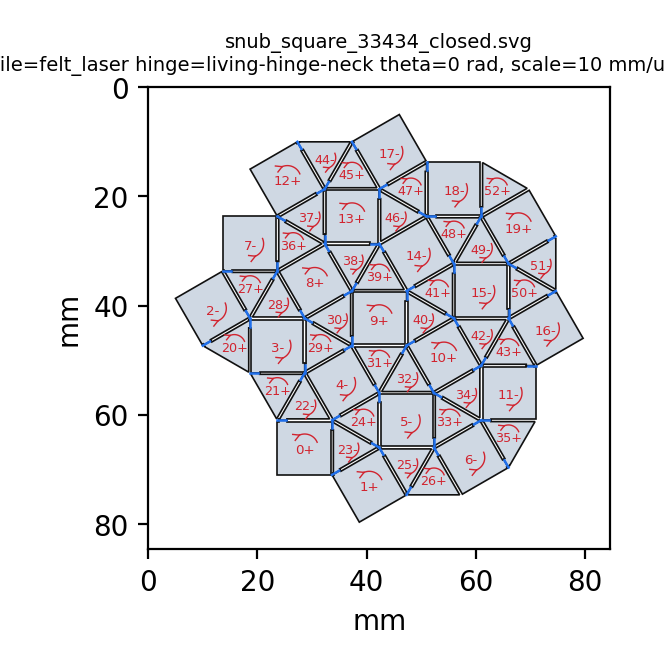
\includegraphics[width=0.32\textwidth]{export/samples/snub_square_33434_closed.png}\hfill
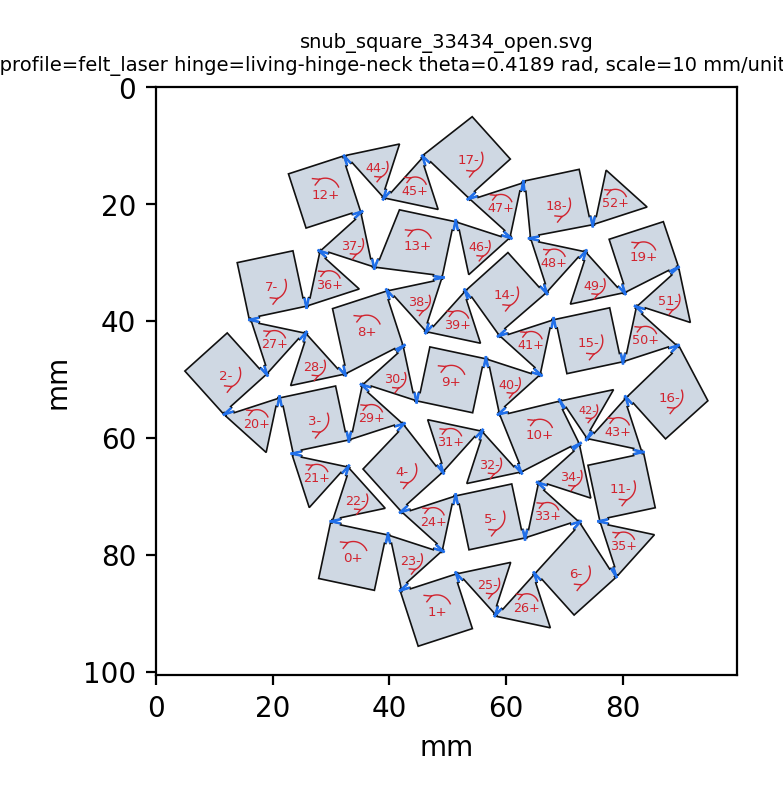
\includegraphics[width=0.32\textwidth]{export/samples/snub_square_33434_open.png}\hfill
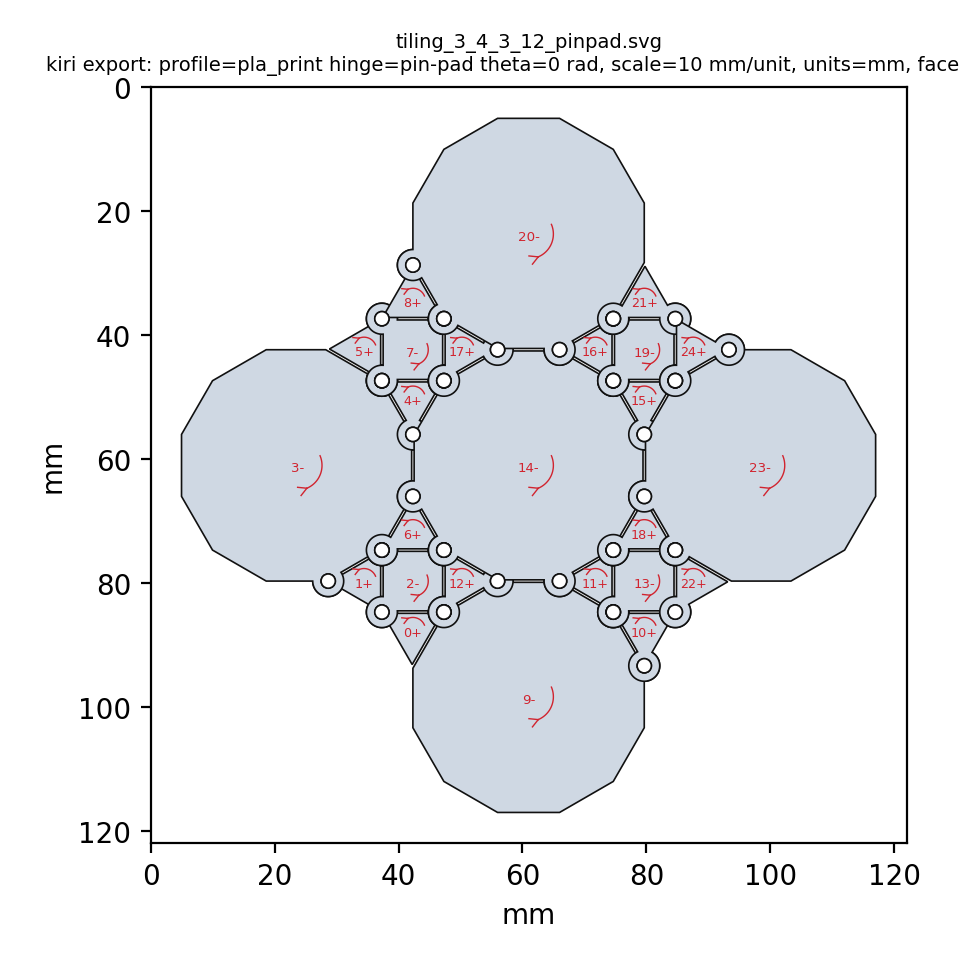
\includegraphics[width=0.32\textwidth]{export/samples/tiling_3_4_3_12_pinpad.png}
\caption{Export samples. Left and centre: the snub square closed and at $0.8\,\theta_{\max}$,
rendered from the SVG by \fn{export/render_svg.py}. Right: the (3,4,3,12) pin-pad set.}
\end{figure}

\paragraph{Validation status.} \fn{kiri_export_tests}: 12 cases, 1\,018 assertions, all
passing. Covered: the profiles and their design rules; the XML checker against hand-written
broken documents; SVG well-formedness, one cut path per face, \fn{viewBox}, mm units, and the
bounding box equal to the input embedding times \fn{--scale}; a neck at every hinge site on both
faces at exactly $\mathrm{setback}\ldots\mathrm{setback}+\mathrm{neck}$ and never on a split or
border side; \textbf{no hinge vertex on any outline} (the anti-pinch property); ear clipping of
a square with a round hole against the exact area; STL closed, consistently oriented, positive
volume, $84+50n$ bytes, and closed again after a round trip through disk; pin-pad giving one
closed body per face stacked over $2t+\mathrm{clearance}$; the zip round trip including a
corrupted-payload rejection and the standard CRC-32 check value \fn{0xCBF43926}; and the 3MF
parts, XML well-formedness, object count and triangle count.
The orchestrator independently re-ran the tests, checked the SVGs with \fn{xmllint}, checked all
three 3MF files with \fn{unzip -t}, and inspected the PNG previews. Gate 8's export half is
recorded PASSED.

\paragraph{Limitations, and the one gate clause that is not met.}
\begin{enumerate}[nosep,leftmargin=6mm]
\item \textbf{No slicer is installed on this machine.} \fn{which prusa-slicer bambu-studio cura
orca-slicer} finds nothing. The 3MF files were validated only by unzipping, checking every part
is well-formed XML, and checking the STL closes after a disk round trip. \textbf{Nobody has
opened them in a slicer}, so MISSION \S5 phase 8's ``export opens in a slicer'' is not verified.
\item \textbf{The pin-pad STL is a plate soup.} A binary STL has no notion of bodies, so
re-reading the pin-pad STL as one mesh reports 2\,304 non-manifold edges --- the 25 plates
overlap over their pads by construction. Each plate alone is closed and consistently oriented,
and the 3MF keeps them as 25 separate objects. \emph{Use the 3MF for pin-pad output.} The
living-hinge STLs are single manifold solids and re-read as closed.
\item ``A neck centred on the hinge vertex'' is impossible as stated; the neck is anchored on
the edge and set back.
\item \textbf{Zero-area cap triangles} from ear-clipping collinear runs: 62 of 1388 on
(3,4,3,12), 72 of 1992 on the snub square. They carry no area and no volume, the solid is still
closed, and slicers drop them --- reported rather than hidden.
\item The pin-pad lobe is a full disc, so it reaches into \emph{every} face at the hinge vertex;
faces in the same $z$ layer then interfere. On (3,4,3,12) at 10\,mm/unit with pad radius 2.5\,mm
it fires at most hinge sites. This is a design-rule violation, named per edge by the CLI, not a
mesh error.
\item Living-hinge necks are full sheet thickness; a real living hinge is usually thinned, which
needs variable-height extrusion.
\item No nesting or part layout; faces are drawn where the kinematics puts them.
\end{enumerate}

%=====================================================================
\section{Dead ends, with the number that killed each}
%=====================================================================

\begin{table}[h]\centering\small
\begin{tabular}{@{}p{42mm}p{55mm}p{55mm}@{}}
\toprule
Idea & Why it was pursued & The number that killed it \\
\midrule
\textbf{R3} bifurcation spectrum / mobility bundle & The only question in the four persona files whose answer nobody in the field knows; targets 2026 \S6 limitation 2 & K3a: $m_{\rm core}\le5$ on \textbf{0 of 167} Delaunay patches, median $m_{\rm core} = 305$, growing roughly linearly with $|F|$. ``Exactly one zero eigenvalue along the uniform branch'' is false for generic finite patches, and the bifurcation question is ill-posed at this mobility \\
\textbf{R1's margin claim} (range-optimal projection) & The headline algorithm of the first commitment & K2b: median relative gain \textbf{0.0000} against the authors' native \texttt{prevent} on 30 live designs; 7 wins, 15 losses, 16 ties. Their optimizer already reaches $\Theta_{\max} = \pi$ on the snub square. The earlier ``86.1\,\% gap closure'' was against our own $X_0$, not their code \\
\textbf{A8} ``Eq.~(2) sufficient but not necessary'' & Would enlarge the deployable class beyond Segall's & Already published: 2025 Fig.~10 shows a deployment-unfriendly tiling deploying with unequal angles, with a photograph; and Dang et al.\ 2021 prove an iff for quads (F20). The existence half is dead on arrival; only the characterization half survives, and it is much harder \\
\textbf{Our Eq.~(9) reconstruction} as a baseline & The only Eq.~(9) available before the native build & F18: the authors' native \texttt{prevent} at published defaults reaches $\Theta_{\max} = \pi$ on the snub square where ours is stuck at 1.646137 for every $\gamma$ in the ladder; and K1c: ours collapses \textbf{109 split edges} to zero length across the population where theirs collapses \textbf{0} \\
\textbf{H-LOC} and every $O(n)$ claim & Would have made R1 \S4 a theorem rather than a broad phase & K2c and the Deriver's round-2 program: $\max_f\|\gamma_f - \bar x_f\|/r_f$ grows \emph{linearly} with patch diameter, 1.414 $\to$ 14.637 over diameters 2.828 $\to$ 26.870 (and 4.62 $\to$ 20.03 in the Deriver's independent run). Refuted, not unproved \\
\textbf{K2c's original PASS} & Was reported as the locality gate passing & The gate statistic is identically $1.000000000001$ by algebra, so its log-log slope is 0 for any input. It can neither pass nor fail informatively. Retracted \\
\textbf{R5 / K5} defect-minimizing orientation as an algorithm & Eq.~(1) knows nothing about whether the closure system has a nearby solution & K5: certified valid $X_0$ on \textbf{0/200} for $\sigma_{\rm def}$, exactly as for $\sigma_{\rm mc}$, and $\Theta_{\max}=0$ on all 400. It fixes the flat sheet ($122\times$ defect reduction, \texttt{POS} 58 $\to$ 186) and does nothing for the deployment \\
\textbf{K6} $0^+$ repair in the null space & The last route to a usable random-graph shape space & Certified $\Theta_{\max}>0$ on \textbf{0/400}; $0^+$-feasible on only 126/400 even with a $\lambda$ ladder and a second stage; the binding failure is \emph{inverted faces} on 51 of the 40-graph subset's 80 design--family lines. Logged as a dead end by D8 \\
\textbf{The naive $\min$-over-roots $\theta_{\max}$} & The obvious closed form & K2a: wrong on 5 of 187 configurations, worst error \textbf{1.047 rad} on \fn{hexagons_R40} --- a third of the entire deployment range \\
\textbf{K1c's rule as written} & The specified false-negative measurement & Self-contradictory: with the crossing clause applied at its own reference range it reports \emph{exactly} 0 on both sources, because ``$\theta^*<\Theta_{\max}$'' and ``$\theta^*$ is a genuine crossing'' cannot both hold. The 65.09\,\% it would otherwise have produced is not a result \\
\bottomrule
\end{tabular}
\end{table}

%=====================================================================
\section{Current state against MISSION \S1, and what remains}
\label{sec:current-state}
%=====================================================================

\subsection{Deliverable by deliverable}

\begin{description}[leftmargin=6mm,style=nextline]
\item[1. \fn{IDEA.md} --- absent.] The chosen idea exists only as decisions D5--D8 in
\fn{STATE.md}. As it stands after D7 and D8 it is: a \emph{characterization} --- exact
closed-form deployment range and a validity certificate for arbitrary-graph kirigami (T1--T6,
validated against brute force), the emptiness result on random graphs (K1a), the Eq.~(9)
false-negative rate (K1c), and the periodic rank and hole-count corrections (F14, F22) ---
together with a constructive half now aimed at \emph{periodic} patterns (R4 achievable
Jacobians, B20 second closed angle), whose kill experiment K7 is still running.
The kill-experiment result is available for every component; the novelty argument is available
from \fn{notes/screen_bundle.md} and \fn{notes/screen_r1.md}. \emph{The file itself has not been
written.}

\item[2. \fn{derivations/core.md} --- present and checked.] Gate 7 PASSED with zero unresolved
disagreements after five Checker rounds and 89\,055 assertions. Three presentational notes
remain open in \fn{check.md} round 5: $A$ written with a closed rather than an open direction
set, the localization wording, and ``exactly one root in $(0,\pi)$'' which should read ``at most
one, namely $\beta_e$''.

\item[3. \fn{code/} --- present, tests passing.] 53 cases / 16\,004 assertions in
\fn{kiri_tests}, 31 / 89\,055 in \fn{derivation_tests}, 12 / 1\,018 in \fn{kiri_export_tests}.
One standing build item, recorded as an orchestrator decision: \textbf{no mobility rank above
700 faces is to be quoted} until \fn{mobility.hpp}'s \fn{matrix_rank} is fixed or the dense path
forced. Every rank-derived number in K3a above $F = 700$ inherits that caveat, including the
median $m_{\rm full}$ and $m_{\rm core}$ and their ranges.

\item[4. \fn{results/} --- partial.] Core validation and ten kill experiments are on disk with
figures. What MISSION \S1 actually asks for --- ``figures comparing baseline (Segall) vs.\ new
method on $\ge20$ graphs, plus one hero example'' --- does \textbf{not} exist. K2b is the nearest
approach and it is a FAIL, so there is currently no metric on which the method beats the
baseline. MISSION \S8's alternative bar is a characterization ``validated on $\ge500$ random
graphs against brute force''; D7 names that as the target and it has \textbf{not} been run:
K2a's exact-versus-bisection validation covers \textbf{187} configurations, not 500, and on
authored tilings rather than random graphs.

\item[5. \fn{export/} --- present.] Two patterns, closed and open, SVG plus STL plus 3MF. The
slicer clause of gate 8 is not met (no slicer installed).

\item[6. \fn{REPORT.md} --- absent.] Phase 10 was never reached.
\end{description}

\subsection{What is established, and would survive a hostile read}

\begin{itemize}[nosep,leftmargin=5mm]
\item The closed-form apparatus is real: the harmonic identity to $4.18\times10^{-12}$ over
207\,096 triples (K1b); exact $\Theta_{\max}$ agreeing with an independent bisection on
\textbf{187/187} configurations to $1.96\times10^{-10}$ (K2a), after the graze correction and the
three-class $\tau=0$ deflation.
\item The validity certificate works and is proved to work:
$\mathrm{POS}\wedge\mathrm{NOOVERLAP}(\varepsilon/2)\wedge\mathrm{NOROOT}$ implies
$\Theta_{\max}\ge\varepsilon$ on \textbf{65/65} configurations where it holds, 0 violations, and
it is a strict inner approximation (173/187 are actually valid).
\item The broad phase is exact, sound with no hypothesis, and empirically tight: pruned and
unpruned $\Theta_{\max}$ agree to $10^{-12}$ on \textbf{285/285} graphs, median 12.7 surviving
pairs per face.
\item 2026 Eq.~(6) has no validity certificate on \textbf{200/200} random graphs, and the
authors' own code confirms it: \textbf{0 of 37} native ladder points on random graphs is valid.
\item Eq.~(9) is blind to the second-order coefficient by construction, and on about one design
in ten of the authors' own output that blindness costs range (K1c, 9.47\,\%).
\item The orientation is a real and unexploited design variable (K5): $122\times$ defect
reduction, $4.7\times$ shorter projection, \texttt{POS} from 58/200 to 186/200 --- and no
deployment benefit whatsoever.
\item The rank corrections: $L = RD$ exactly on 50/50 and 8/8; $\mathrm{rank}(L) = H - \dim Z$;
$H = |E_{\rm hinge}| - |F| + c(\Gamma)$ on 50/50 and 8/8 with notches excluded; and periodic
$\mathrm{rank}(L) = H-1$ on three tori, so 2026 \S4.4 is false as stated for periodic patterns.
\item The authors' extra boundary-component row is an over-constraint (F23), confirmed to
$7.16\times10^{-15}$ over 53 seeds and 20 BFS orders.
\item K7's C1 and C2, as far as they have run: $J(\theta) = \cos(\theta/2)I+\sin(\theta/2)K$
exactly on 30/30 patterns, with $\dim\mathcal K = 2\,\mathrm{rank}\,\mathcal D \in\{0,2,4\}$, and
conformality to at worst $9.7\times10^{-17}$ over 200 angles wherever $\dim\mathcal K\ge1$ ---
which is 2026 \S5.1's ``empirically'' turned into a measurement. And C4 on bounded patches:
$\theta_c = 2\,\mathrm{atan2}(r,q)$ exact to $4.4\times10^{-16}$ on 7/7.
\end{itemize}

\subsection{What remains}

\begin{enumerate}[leftmargin=6mm]
\item \textbf{Finish K7} and write its section into \fn{results/kill/KILL_REPORT.md}. As the data
stands, C1 and C2 pass outright, C4 passes on bounded patches with the hexagon graze as the one
exception, and C3 certifies only 6 of 22 eligible patterns --- below its own $80\,\%$ bar. The
verdict on D8's constructive half turns on C3.
\item \textbf{Write K6's section} into the kill report, and merge the \fn{first_root} fix that
\texttt{experimenter-k6b} died mid-way through, so that K6's certified numbers can be quoted
without a caveat.
\item \textbf{Run the $\ge500$-graph validation} that D7 names and MISSION \S8 requires for the
characterization bar. K2a covers 187 configurations on authored tilings; the exact
$\Theta_{\max}$ and the certificate need to be validated against brute force at that scale, and
the population question raised by K2a --- that random graphs have no embedded projection to
validate on --- has to be answered explicitly rather than by omission.
\item \textbf{Fix \fn{mobility.hpp}'s \fn{matrix_rank}} or force the dense path, so that the
eight unclaimed K3a violators ($F$ from 1644 to 4902) can be resolved.
\item \textbf{Write \fn{IDEA.md} and \fn{REPORT.md}}, which are the two missing MISSION \S1
deliverables. Both are writing tasks over material that already exists; the Writer spec is on
disk at \fn{specs/writer.md} and was never spawned.
\item \textbf{Open a 3MF in a slicer}, or state in the report that gate 8's slicer clause was
never met.
\item \textbf{Decide what the paper claims.} After D7 and D8 the algorithmic half has failed
twice (K2b, K5) and a third time on random graphs (K6). The characterization half is intact and
independently checked. The K7 result decides whether the constructive half moves to periodic
patterns or is dropped, leaving a characterization-and-correction paper.
\end{enumerate}

%=====================================================================
\section{Day 3 (2026-09-04): round 2, the certificate, and the constrained embedding}
%=====================================================================

This chapter picks up where \S\ref{sec:kill} (K7 ``partial, in flight'') and the closing
\S\ref{sec:current-state} left off, at 2026-09-04 03:29 local time. Everything in it happened
inside a single orchestrator session (\texttt{S2} in \fn{STATE.md}'s session log) that ran
across four account session-limit interruptions and one context compaction; the chapter
follows chronological order, not file order, and every number is re-quoted from
\fn{STATE.md}, \fn{results/kill/KILL\_REPORT.md} (which grew from 856 to 2073 lines during the
day), \fn{results/kill/jitter/cert\_diagnosis.md}, \fn{derivations/check.md} Round 6,
\fn{results/core\_validation/referee\_fix.md}, the three hostile reviews under \fn{review/}, and
the two novelty screens \fn{notes/screen\_r2.md} and \fn{notes/screen\_k9.md}.

\subsection{Four session-limit interruptions, and what survived each}

\begin{table}[h]\centering\small
\begin{tabular}{@{}p{20mm}p{62mm}p{62mm}@{}}
\toprule
Interruption & Killed mid-task & What survived \\
\midrule
\#1, 18:53 (reset 22:00 Europe/Istanbul) & \texttt{Experimenter}, \texttt{Checker},
\texttt{Builder-Export} & Tree verified green before respawn (11\,179 assertions); resumed 22:03
with \texttt{experimenter-kill-2}, \texttt{checker-2}, \texttt{builder-export-2}. No data lost. \\
\#2, 02:32 (reset 03:00) & \texttt{experimenter-k6b} mid-fix of the \fn{first\_root} certificate
bug it had itself found; \texttt{experimenter-k7} before it started & The bug report survived in
the session log and was applied by the next K6 agent (\S\ref{sec:day3-k6k7}). K7 restarted clean. \\
\#3, 04:14 (reset 08:00) & \texttt{k7b} (main stage was in fact complete at 33/33, contrary to
the interim ``31/60'' note --- there is no 60-row population), \texttt{writer-k6} (the 988-line
K6 section had already been written), \texttt{jitter} and \texttt{screen-r2} (never started),
\texttt{vault-builder} (graph built, wiki empty), \texttt{theorist-fable} (never wrote) & K7's 33
completed rows and 40 of 50 \texttt{c3} rows; the K6 section text; \fn{round2\_theorist.md} (739
lines) and \fn{round2\_inverse.md} (700 lines), both finished just before the kill. Resumed 11:42
with five respawned agents. \\
\#4, 13:20 (reset 16:40) & \texttt{experimenter-k9} mid-write-up of its own results section &
\fn{results/kill/k9/} was complete on disk; only the KILL\_REPORT prose was missing and was
written after resume at 17:10 (\S\ref{sec:day3-k9}). \\
\bottomrule
\end{tabular}
\caption{Every interruption cost narrative, not data: no kill-experiment CSV was re-run because
of a session limit, and the one live bug (\fn{first\_root}) was caught and logged by the agent
that found it before being killed.}
\end{table}

\subsection{Closing the two results left in flight: K6 final and K7 final}
\label{sec:day3-k6k7}

\paragraph{K6 final.} \S\ref{sec:kill}'s K6 subsection reported the interim state honestly
flagged: \texttt{experimenter-k6b} had found that \fn{validity\_certificate} set
\texttt{cert.first\_root} to the \emph{first} admissible deflated root a
\texttt{(face-pair, vertex, edge)} loop happened to meet, not the \emph{smallest} one, so callers
using it as the supremum of a certified $\varepsilon$ could over-report. Pass v2
(\fn{k6\_full.csv}) had reported exact $\Theta_{\max}>0$ on \textbf{15/200} $\sigma_{\rm mc}$
designs on the strength of that bug; the independent bisection referee agreed on only 13 of the
15, with worst disagreement \textbf{2.4658 rad} (\fn{delaunay\_7}). The three-line fix is at
\fn{code/src/method/contact.cpp:339} --- keep a root only if it is smaller than the incumbent.
Pass v3 (\fn{k6\_final.csv}, the corrected run) gives the final number:
\textbf{certified $\Theta_{\max}>0$ on 0/400}, unchanged from pass v1's headline --- the bug never
manufactured a certificate, only an inflated \emph{exact} $\Theta_{\max}$ where the certified
count was already zero. A confirmatory rerun (\fn{shards\_v4/}) reproduces every aggregate
exactly. The capped 40-graph comparison against the authors' native \fn{prevent} is likewise
$0/80$ from the same flat states. K6's verdict, as printed in \S\ref{sec:kill}, stands:
\textbf{FAIL, 0\,\% against a 20\,\% bar}, on both $\sigma$ families and all four repair
variants, and this is the result that ended the random-graph constructive programme
(decision D8).

\paragraph{K7 final.} The 04:14 interruption had left the \texttt{main} stage looking like
``31/60'' in a hurried interim note; the true state, recovered by re-reading the shard logs, was
that \texttt{main} was complete at \textbf{33/33} and only 10 of 50 \texttt{c3} rows were
outstanding, finished by addressing single patterns with no row recomputed. The completed table:

\begin{table}[h]\centering\footnotesize
\begin{tabular}{@{}p{28mm}p{16mm}p{78mm}p{10mm}@{}}
\toprule
claim & bar & measured & verdict \\
\midrule
C1 affine Jacobian, $J(\theta)=\cos(\theta/2)I+\sin(\theta/2)K$ & $10^{-9}$, $\ge30$ patterns &
$1.37\times10^{-13}$ (fit) / $4.88\times10^{-14}$ (affinity), \textbf{33/33} & \textbf{PASS} \\
C2 exact conformality at every $\theta$ & $10^{-9}$ at 200 angles & $2.31\times10^{-14}$,
\textbf{25/25} of the patterns with $\dim\mathcal K\ge1$ & \textbf{PASS} \\
C3 designable Poisson family, certified $\Theta_{\max}>0$ & $\ge80\,\%$ & \textbf{12/25 = 48\,\%}
(random target); \textbf{0/25} anisotropic target & \textbf{FAIL} \\
C4 closed-form $\theta_c=2\,\mathrm{atan2}(\operatorname{tr}K,1-\det K)$ & $10^{-6}$ &
$5.53\times10^{-14}$ on 32/33 periodic $+$ $4.44\times10^{-16}$ on 7/7 bounded & \textbf{PASS} \\
\bottomrule
\end{tabular}
\end{table}

Two findings sharpen what \S\ref{sec:kill} could only report as ``in flight''. First, the
achievable-set dimension is \emph{not} bounded by shape-space dimension as the spec guessed
(\fn{min(4, 2\,dim\_null)}): \fn{squares\_3x3} has \fn{dim\_null}~$=4$ (six split cuts) yet
$\dim\mathcal K = 0$ --- its $K$ is frozen at a pure rotation ($\operatorname{tr}K=0$,
$\det K=1$) over the whole shape space, so the cell never opens no matter which point of the
null space is chosen. The correct formula, verified on 33/33, is
$\dim\mathcal K = 2\,\operatorname{rank}\mathcal D$. Second, C3's failure is diagnosed, not
merely measured: on 24 of 25 patterns the linear solve hits even the anisotropic target
$K^*=\operatorname{diag}(1,-0.5)$ to $8.9\times10^{-16}$ --- the achievable set really is
(almost) everything --- but the design realising it has $\min_e q_e$ between $-0.22$ and $-46.3$,
i.e.\ it places split cuts that fold inward at $\theta=0^+$. This is the identical mechanism K5,
K6 and F30 name, now reproduced on periodic tori and authored bounded patches that share
\emph{none} of the random-graph construction: \textbf{the $0^+$ obstruction is a property of the
problem, not of one generator.} K7's own verdict: \textbf{C1, C2, C4 pass; C3 fails.} $R4$'s
characterization half survives; its algorithm half does not, and the constructive programme is
still open after K7.

\subsection{The F32 certificate bug: from an 87\,\% false-negative rate to zero}
\label{sec:day3-f32}

A3 (jitter transition, \S\ref{sec:kill}) was designed to separate ``the design space is empty''
from ``our generator fails'', by jittering the eight authored reference tilings continuously with
their combinatorics held fixed. Four of the eight (\fn{rotating\_squares},
\fn{triangles\_alternating}, \fn{kagome\_3636}, \fn{periodic\_squares\_4x4}) turned out to be
\textbf{split-free} under their own $\sigma$: their shape space is a single point, and Eq.~(6)'s
projection sends any jittered interior geometry back to the authored tiling exactly
($\|X_0-X_{\rm base}\|_\infty = 0.0000$ up to amplitude $a=1.0$). Any sentence of the form
``authored tilings pass 8/8'' is therefore really ``4 trivially, 4 substantively''. On the four
split-bearing tilings the exact $\Theta_{\max}$ shows a monotone, sharp transition:
$a^*\in[0.163,0.522]$ median-edge units, width 0.36--0.61 decades under $\sigma_{\rm mc}$.

\textbf{The certificate did not track this at all}, and that was the finding that decided A3's
verdict. At the smallest amplitude $a=0.005$ every split-bearing tiling had exact
$\Theta_{\max}\in[1.0,2.4]$ rad on 20/20 seeds --- yet the certificate passed on 0, 0, 5 and 10 of
those 20 seeds respectively. Over the whole split-bearing ladder, \textbf{1622 of 1859 rows with
$\Theta_{\max}>0$ were not certified: an 87.3\,\% false-negative rate.} A3's verdict as literally
written was FAIL (the ``certified fraction $\approx0$ at the smallest amplitude'' clause fires),
but its stated meaning --- ``the tilings are knife-edge, hence emptiness is generic'' --- was not
supported: what was knife-edge was the certificate's \texttt{NOROOT} clause, not the geometry.
This became fact F32 and spawned a same-day diagnosis task.

\paragraph{Root cause.} \fn{results/kill/jitter/cert\_diagnosis.md} traces the defect to a missing
predicate, not a tolerance. A root of the orientation harmonic $h_{o,\pi}(\theta)$ only says a
vertex $w$ is collinear with the \emph{infinite line} through an edge $(a,b)$; a genuine contact
additionally needs $w$ on the \emph{segment}, $0\le\langle w-a,b-a\rangle\le|b-a|^2$. The exact
scan's \fn{contact\_angles} applies that interval test; the certificate's \texttt{NOROOT} scan did
not --- and this was not an implementation slip but a deliberate weakening stated in
\fn{derivations/core.md} T5.2b.0(iii). Five replayed rows show the mechanism directly: all 168
roots the certificate found in $(0,\varepsilon)$ on those rows had the vertex \textbf{off the
segment} --- projection parameters running to 6.78 edge lengths past the far endpoint on
\fn{tiling\_3\_4\_3\_12} and $-3.0$/$+4.0$ on \fn{hexagons\_auto}. Of the four candidate causes
tested (permanent-incidence roots, graze admission, predicate mismatch, chart singularity), only
the predicate mismatch was confirmed.

\paragraph{The fix.} Nine lines in \fn{contact.cpp}: build the same squared-length and projection
harmonics the exact scan uses and keep only roots satisfying the interval test, inclusive at
tolerance $10^{-12}\cdot(|L_2.p|+L_2.\mathrm{amp}())$. A new field
\fn{n\_roots\_inadmissible} reports how many roots the filter removed, for diagnostics only.
Regression test (\fn{code/tests/test\_method.cpp}): without the fix, 5 of 12 assertions fail; with
it, all pass, and the two pre-existing certificate tests needed their reference rescans widened
from $\varepsilon=1.2$ to $3.0$ because almost no root is admissible below 3~rad on the regular
patterns. Full suites: \textbf{\fn{kiri\_tests} 66/66, 16\,283 assertions; \fn{derivation\_tests}
31/31, 89\,055 assertions.}

\paragraph{Re-measurement.} On the same 6416 jitter rows, certified count rises from 3445
(53.7\,\%) to \textbf{5064 (78.9\,\%)}, and the certificate becomes \emph{exact} on this corpus:
the 5064 certified rows are precisely the 5064 rows with exact $\Theta_{\max}\ge\varepsilon$, in
both directions, with zero unsound rows.

\begin{table}[h]\centering\small
\begin{tabular}{@{}lrr@{}}
\toprule
metric ($\varepsilon=0.006$, 6416 rows) & before & after \\
\midrule
certified & 3445 (53.7\,\%) & \textbf{5064 (78.9\,\%)} \\
certified, split-bearing rows only & 237 / 3208 (7.4\,\%) & \textbf{1856 / 3208 (57.9\,\%)} \\
split-bearing $\Theta_{\max}\ge1$ rad, not certified & 1010 / 1161 (\textbf{87.0\,\%}) &
\textbf{0 / 1161 (0.0\,\%)} \\
rows with $\Theta_{\max}\ge\varepsilon$, not certified & 1619 / 5064 (32.0\,\%) &
\textbf{0 / 5064 (0.0\,\%)} \\
certified but $\Theta_{\max}<\varepsilon$ (unsound) & 0 & \textbf{0} \\
\bottomrule
\end{tabular}
\end{table}

Downstream, \textbf{K2a's headline moves and strengthens}: certificate-implies-bisection
soundness held on 65/65 configurations before the fix and holds on \textbf{173/173} after, with
zero violations either way, and the corpus's actually-valid count (173/187) is now met
\emph{exactly} --- the sentence ``the certificate is a strict inner approximation, 65 certified
against 173 valid'' is withdrawn and replaced by ``173 certified against 173 valid, exact on this
corpus''. \textbf{K5 and K6 are unaffected}: both fail because the exact scan finds a genuine
$0^+$ split-duplicate collision, on the segment, which a weaker \texttt{NOROOT} cannot manufacture
away; K5's re-run and K6's smoke re-run reproduce their recorded numbers exactly.

\paragraph{Checker Round 6.} Fresh context, scope the amendment above against T3, T4.1b, T4.2,
T5. \textbf{33 test cases, 89\,074 assertions, 0 failures.} Three findings:

\begin{enumerate}[nosep,leftmargin=5mm]
\item \textbf{Soundness of the amended certificate: VERIFIED}, closing two gaps the diagnosis had
not fully proved --- Case A's substitute root at $\beta_e$ is admissible because
$\langle w-a,b-a\rangle = LL'$ with $0<L'\le L$ (measured on 9642 pairs, 580 exactly at the
closed-interval endpoint $L'=L$, i.e.\ every regular tiling's unjittered pair), and a role-swapped
pair repairs a second, previously unnamed gap in the [D2] interior sub-case. [D3]'s extra atoms
are withdrawn as unnecessary under a new stated hypothesis (H6, no straight vertices): the code
was already right.
\item \textbf{Completeness is FALSE, and this does not generalize from the jitter corpus.} The
amended \texttt{NOROOT}$_{\rm adm}(\varepsilon)$ is exactly $\varepsilon\le\theta_1(X)=\min\mathcal
C(X)$, the \emph{first} contact angle, while $U(\varepsilon)$ only asks $\varepsilon\le\Theta_{\max}$.
The two coincide only when the first contact is already an overlap transition --- no graze. The
counterexample is on the project's own T4.2 table: \fn{hexagons\_auto} at $X_0$ has
$\theta_1=\pi/3=1.047198$ (a graze) and $\Theta_{\max}=2\pi/3=2.094395$; at $\varepsilon=\pi/2$
the true range clears but the certificate reports \texttt{NOROOT}~=~false. The certificate is
\textbf{exact for $\varepsilon$ below the first graze, an inner approximation above it}, and the
jitter re-measurement's 0/5064 exceptions is a property of \emph{(corpus, $\varepsilon$)}, not of
the certificate in general --- tagged \textsc{conjecture} (T5.2b-complete) for the open question
of a bounded-atom-count complete description.
\item \textbf{A second referee artefact, localized and left unfixed here.} B4's \fn{voronoi\_93}
row reports exact scan $0.2484$ against bisection referee $0$; a $1200\times1200$ grid and 17\,280
radial probes find zero common interior points, so the scan is right. The referee's
\fn{polygons\_overlap} shrinks each polygon's copy of a \emph{shared hinge vertex} by a different
displacement, producing orientation determinants of size $10^{-11}$--$10^{-17}$ whose sign flips
with the shrink parameter and with $\theta$ --- non-monotonically. The bias is downward only, so
no FAIL verdict built on it is compromised, but \fn{theta\_bisect} could not be quoted as ground
truth until fixed (\S\ref{sec:day3-f34}).
\end{enumerate}

\subsection{Round-2 escalation, and decision D9}

Three consecutive constructive round-2 ideas died in the same session: T-1 vertex balance
(FAIL, reflex corners), B4 boundary drop (FAIL, 1/400 refereed), K8a expansive-cone LP (FAIL,
0/100, dual-certified structural on 84/100) --- detailed in \S\ref{sec:day3-round2}. With one
candidate (B3) still running, the orchestrator wrote \fn{ESCALATION.md}, invoking MISSION \S9's
stop condition. It listed what was already verified and paper-ready (the T1--T7 calculus, the
sound Round-6 certificate, the periodic affine theorem, the structural non-deployability results,
the errata) against what MISSION \S8 still asked for --- a constructive algorithm beating the
Segall baseline on $\ge20$ graphs, which every attempt so far had failed on the same $0^+$
split-cut contact. Four options were listed, with option 1 (reframe as characterization plus
impossibility) as the orchestrator's running baseline and option 2 (change the embedding, not the
graph, via a convexity-constrained solve) run in parallel as a single two-hour kill test.

\textbf{Resolution, same day 17:15.} K9 (option 2) returned \textbf{36/400 exact, 32--36
refereed} deployable random graphs against zero for every baseline --- below the 10\,\% bar by
4--8 designs, but above MISSION \S8c's ``$\ge20$ graphs'' by a wide margin against a baseline of
zero. \textbf{Decision D9}: option 2 becomes the constructive half of the deliverable, with a
push phase (K9b) to follow, a referee fix (F34), Builder-Method consolidation, a hero design,
export, and the Writer. The paper framing settled here --- exact calculus plus sound certificate
plus certified impossibility of the published embedding plus the constrained embedding that
deploys --- is the one carried into \S\ref{sec:day3-paper}. Escalation closed; no human decision
was required.

\subsection{T-1, B4, K8a, B3: four more negative results, and what each establishes structurally}
\label{sec:day3-round2}

\begin{table}[h]\centering\small
\begin{tabular}{@{}p{9mm}p{18mm}p{115mm}@{}}
\toprule
Exp. & Verdict & Key number and structural finding \\
\midrule
T-1 & \textbf{FAIL} & Of 1968 balanced pure-hinge vertices (\texttt{BAL} holds exactly, max
$|\delta_v|=2\times10^{-14}$), \textbf{1966/1968} non-positive-margin incidences sit at a
\textbf{reflex} corner created by Eq.~(6)'s unconstrained projection (0 non-convex faces at input
$\to$ 22\,103/156\,220 at $X_0$). At a convex corner the margin is a disjunction
($\max(-g_1,-g_2)$); at a reflex corner it is a conjunction ($\min(-g_1,-g_2)$), which is the one
that fails. Corr($\delta,\mu$) on touched vertices $\approx0$. Weight transfers to convexity as a
constraint (K9). \\
B4 & \textbf{FAIL} & Dropping 2026 Eq.~(4)'s fixed-boundary rows entirely: exact
$\Theta_{\max}>0$ on \textbf{2/400} (0.50\,\%) against a 10\,\% bar; \textbf{1/2} refereed after
the F34 fix. Dimension count exactly right ($\dim\_null(\rm free)-\dim\_null(\rm fixed) =
|V_\partial|-1$ on 400/400), and split-only feasibility triples under $\sigma_{\rm mc}$ and
reaches 200/200 under $\sigma_{\rm def}$ --- but the primary (convexity-adjacent) objective still
fails on all but 3/200, because $|V_\partial|\approx33$ extra handles are dwarfed by 126--321
simultaneous split-sign constraints. \textbf{The fixed boundary is not what empties the space};
K7's 4/12 torus rate is not explained by absence of \(B\). \\
K8a & \textbf{FAIL} (bar $\ge20/100$); \textbf{PASS} on the hard soundness control (4/4) & LP over
the flex cone \fn{ker}\,$A$ finds a strictly positive non-uniform margin on \textbf{0/100} random
graphs at $X_{\rm ini}$ and $X_0$; on \textbf{84/100} the Frank--Wolfe dual gives an approximate
Farkas certificate ($<10^{-6}$) that \emph{no} flex --- uniform or not --- separates every cut and
corner at first order. One genuine rescue exists (\fn{snub\_square\_R20\_s1}, margin
$4.31\times10^{-2}$), never on a random graph. Euler-step sanity 72/72 collision-free. \emph{The
emptiness is structural}, not one bad ray of a high-dimensional cone --- the strongest defence
against the ``it's just your two orientation heuristics'' objection. \\
B3 & theorem \textbf{PASS} (repaired); algorithm \textbf{FAIL}, hard-fail clause triggered &
Summing one representative \emph{preimage} per translation class (not per quotient edge) repairs
the identity to $W+R=\det P_0\cdot\operatorname{tr}K$ at $10^{-15}$ on 30/33 patterns: \(\tau^* -
\operatorname{tr}K = -R/\det P_0\) exactly. AUC($\operatorname{tr}K-\tau^*$) for
\texttt{min\,q\,$>$\,0} is 0.980 (bar 0.80, PASS) --- but \textbf{spread($W$)/spread($\det
P_0\operatorname{tr}K$) over $\mathcal K$ has median 0.727, max 1.401}: the HARD-FAIL clause the
Critic named fires, because $W$ moves nearly as much as the budget it is meant to gate, so
$\tau^*$ is a penalty on the design, not a threshold on the pattern. Constrained re-solve:
certified $12\to13$/$14$ (inside binomial noise), $12\to2$ at $\delta=0.5$ (target abandoned,
Frobenius drift up to 589). \\
\bottomrule
\end{tabular}
\caption{All four round-2 constructive attempts fail their own bars; three of the four (T-1, K8a,
B3) fail while confirming a genuine, checked mechanism that later feeds K9 or is folded into the
paper's negative-result apparatus. Only B4's mechanism (extra boundary handles) turns out not to
matter.}
\end{table}

\subsection{K9: the first non-zero constructive result on random graphs}
\label{sec:day3-k9}

T-1's finding --- that the $0^+$ jam sits almost entirely at reflex corners the projection itself
creates --- motivates a direct fix: constrain the null-space embedding to keep every corner
strictly convex, and add back the split-inward sign condition K6 already used.

\[
\text{minimise } \|X(t)-X_{\rm ini}\|_F^2 \quad\text{subject to}\quad
\mathrm{cross}_i(t)\ge\delta \ \ (\text{every corner}), \qquad
[\, q_e(t)\ge\delta' \ \ (\text{every split cut}) \,]
\]

inside the affine shape space $X(t)=X_0+\Phi t$, with $\mathrm{cross} =
\det(X[v]-X[v_{\rm prev}], X[v_{\rm next}]-X[v])$ positive exactly at a strictly convex corner of
a CCW face. Every corner strictly convex implies every face convex and positively oriented, so
this constraint \emph{subsumes} K6's face-area constraint. The feasible set is not convex, so the
solve (\fn{code/src/method/convex\_embed.{hpp,cpp}}) is a stated heuristic: a softplus-penalised
continuation over three target scales, then a log-barrier refinement keeping only strictly
feasible iterates, on the same 200 K1a/K5/K6 graphs under both $\sigma$, 400 designs, exactly the
population K5/K6 measured. \textbf{PASS rule: refereed exact $\Theta_{\max}>0$ on $\ge10\,\%$
(\(\ge40\)) of 400.}

\begin{table}[h]\centering\small
\begin{tabular}{@{}p{48mm}p{28mm}p{28mm}p{40mm}@{}}
\toprule
quantity & $X_0$ (control) & (a) convexity only & (b) convexity $+$ split \\
\midrule
convex-feasible & 79/400 (19.8\,\%) & \textbf{115/400 (28.8\,\%)} & 30/400 (7.5\,\%) \\
\textbf{exact $\Theta_{\max}>0$} & 0 & 0 & \textbf{36/400 (9.0\,\%)} \\
refereed at shrink $10^{-9}$ (post-F34, \S\ref{sec:day3-f34}) & 0 & 0 & \textbf{36} \\
certified & 0 & 0 & \textbf{36} \\
binding contact at $\Theta_{\max}=0$ & split-inward 400 & split-inward 400 & split-inward 260,
inverted 72, vertex-edge 32 \\
\bottomrule
\end{tabular}
\end{table}

Arm (a) --- convexity alone --- raises convex feasibility to 115/400 and buys \textbf{exactly
zero} deployment range: the binding contact stays split-inward on all 400. \textbf{Convexity is
necessary, not sufficient}; the two constraints together are what moves the count off zero. Over
the 36 positives: exact $\Theta_{\max}$ median \textbf{0.249}, min 0.027, max
\textbf{1.997}~rad; 33/36 have $\varepsilon_{\max}\ge0.1$~rad; by family delaunay 25, voronoi 10,
quad\_random 1; taking the better $\sigma$ per graph, \textbf{33 of the 200 graphs} carry at
least one deployable design. Only 23 of the 36 are actually \fn{b\_feasible} at the full margin
$\delta'$ --- 13 miss the margin the solver aimed at and deploy anyway, foreshadowing K9b's
finding that margin feasibility is a sufficient handle on the $0^+$ cone, not a necessary one.

\subsubsection{The F34 referee artefact, and the fix}
\label{sec:day3-f34}

Four of the 36 exact positives (\fn{delaunay} 13, 40, 103, 190, all $\sigma_{\rm mc}$) refereed as
$\Theta_{\rm bisect}=0$ at the historical shrink $10^{-12}$. Tracing every one
(\fn{code/apps/dbg\_k9.cpp}) finds the bisection's early-exit \fn{has\_collision}$(10^{-7})$
firing on a pair of \textbf{hinge-adjacent} faces that touch at the pin by construction, and firing
\emph{non-monotonically} in $\theta$ (true at $10^{-8},10^{-7},10^{-5}$; false at
$10^{-9},10^{-6},10^{-4},\dots$) --- numerical noise of the near-flat state, the same
\fn{shrink\_poly} defect Round 6 had already localized on B4's \fn{voronoi\_93}
(\S\ref{sec:day3-f32}). \textbf{The fix} (\fn{results/core\_validation/referee\_fix.md}):
\fn{polygons\_overlap} no longer shrinks anything. It decides whether the \emph{open interiors}
meet exactly, by splitting each polygon's boundary at every intersection with the other and
classifying the midpoint of every resulting piece with a three-state point-in-polygon test, with
containment as a fallback and the orientation predicate snapped to zero by a scale-free relative
tolerance. Cost: about $3\times$ slower per pair (K2a wall $13.6\to39.6$~s for the whole 187-design
run). New tests in \fn{code/tests/test\_collision.cpp}, written first and failing against the old
predicate on the \fn{voronoi\_93} polygons (10/10 wrong before, correct after); full suites
\textbf{\fn{kiri\_tests} 84/84, 17\,203 assertions; \fn{derivation\_tests} 33/33, 89\,074
assertions}.

\textbf{Re-referee, before vs.\ after, isolated from concurrent \fn{contact.cpp} changes by a
baseline binary with only \fn{collision.cpp} reverted:}

\begin{center}\footnotesize
\begin{tabular}{@{}lrr@{}}
\toprule
population & before & after \\
\midrule
K2a: min-over-roots vs.\ bisection, tol $10^{-6}$ & 149/187 & \textbf{182/187} \\
K2a: worst gap at shrink $10^{-9}$ & $1.956\times10^{-7}$ & \textbf{$2.579\times10^{-8}$} \\
B4 \fn{voronoi\_93}, referee (scan says $0.2484$) & $0.000000$ & \textbf{$0.248400$} \\
K5: \fn{sigma\_def} embeds an overlap-free $X_0$ & 114/200 (57.0\,\%) & \textbf{123/200 (61.5\,\%)} \\
K6: exact $\Theta_{\max}>0$ (primary, no-native) & 0/400 & \textbf{2/400} (both still uncertified) \\
K9: refereed $\Theta_{\rm bisect}>0$, arm (b) & 32/400 & \textbf{36/400} \\
K9: worst $|\theta_{\rm exact}-\theta_{\rm bisect}|$ & $3.020\times10^{-1}$ & \textbf{0} \\
\bottomrule
\end{tabular}
\end{center}

\textbf{No verdict moves.} K2a PASS, K5 PASS, K6 FAIL ($2/400=0.5\,\%$ against a 20\,\% bar), K9
FAIL ($36/400=9.0\,\%$ against a 10\,\% bar), B4 unchanged. The old predicate's bias was
one-sided --- it only ever reported collisions that were not there --- so every FAIL verdict built
on it was conservative and nothing flips; what changes is that K9's headline collapses to one
number, \textbf{36/400 exact and 36/400 refereed}, and the referee becomes usable as an
independent cross-check without a shrink-dependence caveat (though it remains a resolution-limited
bisection on a 4000-point grid, not the ground truth --- that is still the exact T4.2$''$ scan).

\paragraph{K9's verdict.} \textbf{FAIL by 4--8 designs against a 10\,\% bar}, and the first
constructive foothold this project has produced: every comparable baseline on the identical 400
designs is exactly zero --- Eq.~(6) alone (K1a), $\sigma_{\rm mc}$/$\sigma_{\rm def}$ (K5), all
four K6 repairs, convexity alone, B4, K8a, and the authors' native \fn{prevent} (0/80 on the
capped comparison). The expansive-cone LP finds no witness on the 30 (b)-feasible designs, but on
23 of them $\sigma$ is directly measured to be \emph{inside} $P(X)$ ($\min q>0$ and $\min\mu>0$),
so the LP's $0/30$ is \textbf{cone\_lp non-convergence, not emptiness} --- K8a's dual
``certificates'' on 84/100 must be read with that caveat attached (dual bounds there run
$2$--$5\times10^{-2}$, far above the $10^{-7}$ threshold that would license a claim of
infeasibility).

\subsection{K9b: pushing the constrained embedding}
\label{sec:day3-k9b}

K9b holds the population, the shape space and the certificate fixed and pushes only the solver
--- more restarts (8 Gaussian $+ t=0$ vs.\ K9's 3, plus two warm starts), a $\delta=\delta'$
sweep over $\{10^{-4},10^{-3},3\times10^{-3},10^{-2}\}\cdot\mathrm{med}^2$, and a gated stage-2
range-optimisation pass (\fn{range\_opt.hpp}'s analytic-gradient objective, accepted only if the
exact constraints still hold and $\Theta_{\max}$ actually improved).

\begin{table}[h]\centering\small
\begin{tabular}{@{}lrrr@{}}
\toprule
quantity & K9 (b) & K9b sweep & best over both \\
\midrule
exact $\Theta_{\max}>0$ & 36/400 (9.0\,\%) & \textbf{28/400 (7.0\,\%)} & \textbf{37/400 (9.25\,\%)} \\
refereed at shrink $10^{-9}$ & 36 & 28 & 37 \\
$\varepsilon_{\max}\ge0.1$ rad & 33 & 16 & \textbf{34} \\
graphs with $\ge1$ deployable design (of 200) & 33 & 26 & \textbf{34} \\
\bottomrule
\end{tabular}
\end{table}

\textbf{More search made the raw count worse.} Only the $\delta$ sweep paid: among K9b's 28
positives the winning margin is $10^{-2}\cdot\mathrm{med}^2$ (ten times K9's default) on 15 of
28, K9's own $10^{-3}$ on 12. Restarts and extra barrier stages did not pay, and stage~2 supplied
the accepted point on only 2 of 28 positives, because it was gated on $\Theta_{\max}>0$ and so
never ran on the feasible-but-jammed designs where it might have mattered. \textbf{The 9 designs
K9b lost are the informative result.} All nine are \fn{delaunay}; on all nine K9b's returned
point is \emph{exactly feasible} --- every corner cross and every split sign clears the margin ---
and still has $\Theta_{\max}=0$, binding on vertex-edge. Two different solver runs land on
different points inside the \emph{same} feasible set, one deployable and one not:
\textbf{margin feasibility does not determine deployability}, and the proximity objective
$\|X-X_{\rm ini}\|$ that picks the point inside the feasible set is not aligned with deployment
range. That, not the search budget, is what caps the yield near 9\,\%: only 13 of K9b's 28
feasible designs are positive, and only 13 of its 28 positives are margin-feasible.

\begin{figure}[h]\centering
\includegraphics[width=0.85\textwidth]{results/kill/k9b/k9b_gallery.png}
\caption{24 random graphs from K9b's own run, closed (left) and at $\theta=\Theta_{\max}/2$
(right), $F$ from 101 to 442, $\Theta_{\max}/2$ from 0.002 to 0.914~rad. The lower rows are
visually near-indistinguishable from the closed state --- roughly a third of positives sit below
0.1~rad of half-range --- which is exactly the constructive-review's ``existence, not
prevalence'' reading (\S\ref{sec:day3-reviews}).}
\label{fig:k9b-gallery}
\end{figure}

\textbf{Verdict: FAIL} --- the bar is missed by 3 designs at best (37/400 over both solver
configurations) rather than 4--8, and the constructive claim carried forward is the same in kind
and firmer in evidence: \textbf{37 random graphs deploy from a constrained embedding, and none
deploy without it.} F36 is amended: the $\sim9\,\%$ yield is \textbf{basin-selected, not
budget-limited} --- $4\times$ search budget with the same proximity objective moves the certified
count \emph{down}, and 9 of K9's own positives turn out to be margin-feasible points with
$\Theta_{\max}=0$ under the pushed solver.

\subsection{Three hostile reviews}
\label{sec:day3-reviews}

Three adversarial reviews were commissioned in parallel over the finished bundle:
\fn{review/theory\_review.md} (T1--T7, K7, F35, a TOG/rigidity-theory referee), \fn{review/negative\_
review.md} (the K1a/K5/K6/B4 emptiness claims, played as a hostile referee response defending the
2026 paper), and \fn{review/constructive\_review.md} (K9/K9b, a computational-design reviewer
skeptical of barrier-method claims dressed as theory). None offers unqualified praise; each ends
with a rejection sentence and a concrete rebuttal or fix.

\paragraph{Theory review.} Classifies every theorem TRIVIAL-CONSEQUENCE-OF-KNOWN, KNOWN, or NEW,
with a dismissal sentence and a rebuttal for each. Verdicts: T1 (trig-linear) and T2 (no-locking)
are the 2D specialization of Tay--Whiteley motion assignment, textbook once the correspondence is
known --- keep T2's corollary (mobility never terminates kinematically, licensing T4's contact-list
completeness) but drop the theorem-with-corollaries framing. T3 (harmonic predicates) is
Weierstrass-level algebra in \emph{form}, but the fact that the coefficients are quadratic in the
design coordinates $t$ --- not just in $\theta$ --- is load-bearing for everything downstream and
is NEW relative to the closest prior use (Grima et al.\ 2012's hinge-adjacent, collinearity-assumed
special case). T4 (exact $\Theta_{\max}$, graze handling) is the review's top-ranked result: it
falsifies the project's own round-1 claim and an implicit assumption of the 2026 paper
($\Theta_{\max}=\min_e\beta_e$) \textbf{on the paper's own triangle figure}, and ``any
implementation that assumes T4.3 will be wrong on the paper's own figures''. T5 (the certificate)
is standard verified-computation methodology in a new domain, with the withdrawal history itself
read as evidence the project's error-catching process works. T6 (implicit-function gradients) and
K7-C4 (closed-form $\theta_c$) are demoted to remarks --- one-line algebra once T1/C1 exist. T7
(the periodic rank off-by-one) is a small but concrete, checked correction to 2026 \S4.4. The
review's own top-5 ranking places \textbf{K7-C3's FAIL, read as a positive result about the whole
bundle}, at \#3: it independently reproduces the $\theta=0^+$ collision obstruction on a
population sharing none of K5/K6's construction, which a referee is said to ``respect... far more
than another PASS.''

\paragraph{Negative review (hostile referee response).} Argues the 2026 paper never claims to
deploy \emph{random} planar graphs --- its ``arbitrary'' means combinatorially unrestricted
(non-2-colourable, aperiodic, with holes), demonstrated by one hand-picked example per exclusion,
never over a population. It finds the ``0/400'' figures are honestly scoped in every
\fn{KILL\_REPORT.md} section individually, but flags a real risk of \emph{implication through
juxtaposition} in \fn{STATE.md}'s compressed one-liners, and supplies five wording corrections
(Table~\ref{tab:day3-wording}). It also computes that across roughly 1600 (design, $\sigma$) slots
derived from the 200-graph population, the authors' native \fn{prevent} was actually invoked on
only \textbf{8 designs total} (K6's capped native run) --- because on every other slot the pattern
was already invalid before \fn{prevent} had anything to work with --- and recommends the one
experiment that would close the gap: run native \fn{prevent} unconditionally on all 200 graphs
$\times$ 2 $\sigma$, estimated at 1--7 hours wall time, embarrassingly parallel on the existing
12-shard infrastructure. It reads 2026 \S6 Limitation 1 (quoted in full) as conceding exactly R1's
problem statement --- membership in the shape space does not imply a valid or useful embedding,
and the authors have no a-priori certificate --- but \emph{not} conceding genericity of emptiness,
which is this project's own measured contribution.

\begin{table}[h]\centering\small
\begin{tabular}{@{}p{58mm}p{75mm}@{}}
\toprule
As written & Corrected \\
\midrule
``The whole design space, all four strategies, is 0/400 certified.'' (K6) & ``All four of our own
repair strategies are 0/400 certified; the authors' native \fn{prevent}, tested separately on the
8 of these 400 designs that reached a valid flat state, is also 0/8.'' \\
``on random graphs the Tutte auxetic shape space ... contains no sampled/projected point with
positive deployment range (0/400)'' (F30) & ``no \emph{sampled or Eq.~(6)/repair-projected} point
... has positive range; whether the true infinite-dimensional space contains such a point is not
decided by sampling.'' \\
K1a ``PASS-emptiness'' quoted downstream without qualifier & keep ``under $\sigma_{\rm mc}$''
attached every time. \\
F27 ``RANGE-MARGIN CLAIM DEAD'' & ``the \emph{median} margin claim is dead (0\,\% vs.\ a 25\,\%
bar); the method still wins on 7/30 designs, by up to 10.6\,\%.'' \\
F36 ``FIRST NON-ZERO CONSTRUCTIVE RESULT ON RANDOM GRAPHS'' & accurate as printed, already hedged
by the 36/400 vs.\ 40/400 bar miss --- no correction needed. \\
\bottomrule
\end{tabular}
\caption{Wording corrections from \fn{review/negative\_review.md}, applied to this notebook's own
phrasing above.}
\label{tab:day3-wording}
\end{table}

\paragraph{Constructive review (K9/K9b).} The harshest of the three. Reads 36--37/400 as
``a curiosity that the authors correctly did not oversell, but is too thin to anchor a paper on
its own'': only 13--16 of 28--36 positives clear $\varepsilon_{\max}\ge0.1$~rad, roughly a third
sit below 0.03~rad (``a barely-perceptible wobble, not a deployment''), and the gallery figure
(Fig.~\ref{fig:k9b-gallery}, above) makes the bottom third visually indistinguishable from
closed. Mechanically, it calls the method ``add two constraints to a barrier solver'' --- nothing
about the optimizer is novel --- and identifies K9b's own finding (feasibility does not determine
deployability) as \emph{the} most important and most self-damaging result in the set, because it
shows the constraint pair is a necessary filter, not the mechanism, and the real selector is
unidentified. On fairness it notes the native-\fn{prevent} comparison covers only 80 of 400
designs, capped by a runtime timeout rather than a principled sampling choice, and recommends
finishing it. Its proposed rejection sentence: ``the paper proposes two barrier constraints inside
an existing null-space projection and demonstrates a 9\,\% yield with median opening under
$15^\circ$, on an incomplete baseline comparison ... falling short of its own pre-registered
10\,\% bar and offering no characterization of why the constraint pair succeeds where it does.''
Its own suggested rebuttal --- accept 9\,\% as a floor against seven baselines that are all exactly
zero, and reframe the headline as ``a constrained-embedding lower bound on the non-empty fraction
of the random-graph design space'' rather than any deployability claim --- is the wording adopted
in \S\ref{sec:day3-paper} below.

\subsection{The current paper skeleton}
\label{sec:day3-paper}

Following D9's framing and the three reviews' corrections, the paper the bundle currently supports
is a \textbf{characterization-and-impossibility paper with a small, certified constructive
residue}, not an algorithm paper. Its shape, as of this chapter:

\begin{enumerate}[leftmargin=6mm]
\item \textbf{Exact deployment calculus (T1--T7).} Trig-linear deployment, no-locking, harmonic
predicates with the systematic-degeneracy catalogue, exact $\Theta_{\max}$ with graze handling
(the theory review's top-ranked result, falsifying $\Theta_{\max}=\min_e\beta_e$ on the paper's
own triangle figure), exact gradients, and the periodic rank off-by-one correction to 2026
\S4.4 --- five checker rounds, zero unresolved disagreements, 89\,074 assertions.
\item \textbf{The sound certificate (Round 6).} $\mathrm{POS}\wedge\mathrm{NOOVERLAP}(\varepsilon/2)
\wedge\mathrm{NOROOT}_{\rm adm}$ proved sound after the F32 amendment, exact on the K2a/A3 corpora,
and honestly stated as an inner approximation above the first graze --- with the hexagon
counterexample printed, not hidden.
\item \textbf{The periodic affine theorem (K7 C1/C2/C4).} $J(\theta)=\cos(\theta/2)I+
\sin(\theta/2)K$ exact on 33/33 patterns, $\dim\mathcal K = 2\operatorname{rank}\mathcal D$, exact
conformality at every $\theta$ (proving 2026 \S5.1's ``empirically''), and the closed-form second
closed angle.
\item \textbf{Certified structural non-deployability of random-graph patches.} Both uniform
(K1a/K5/K6/B4) and non-uniform (K8a) orientations, on the identical 400-design population,
including near-Farkas dual certificates on 84/100 graphs that no flex at all --- uniform or not
--- clears every split and corner at first order.
\item \textbf{The sharp jitter transition (A3), correctly attributed to geometry.} $a^*\in
[0.16,0.52]$ median-edge units on the four split-bearing authored tilings after the certificate
fix, with the local mechanism (T-1: reflex corners created by Eq.~(6)'s projection, not by the
graph) identified and measured.
\item \textbf{The constructive residue (K9/K9b).} 37/400 random graphs deploy under a convexity
$+$ split-inward constrained embedding, none deploy without it, reported with every qualifier the
constructive review demanded --- yield rate, $\varepsilon_{\max}$ distribution, Delaunay bias, and
the feasibility-does-not-imply-deployability caveat as its own figure, not a footnote.
\item \textbf{Errata against the authors' own code.} The rank claim (F14/F22), the boundary
over-constraint (F23), and the 9.47\,\% silent Eq.~(9) re-closure rate (K1c).
\end{enumerate}

What is \emph{not} in this skeleton, per the reviews above: any sentence claiming the published
pipeline (including native \fn{prevent}) achieves zero on random graphs unconditionally (only 8
designs were ever run through it; the full 400-design run is the negative review's proposed
closer), any unqualified ``first deployable random-graph kirigami'' claim, and any framing of K9b's
loss of 9 designs as noise rather than as the paper's own evidence that the constraint pair is
necessary but not sufficient.


%=====================================================================
\appendix
\section{Verified facts F1--F30, verbatim from \texttt{STATE.md}}
Reproduced literally, in the file's own order, with Greek letters and mathematical symbols
transliterated to ASCII so the block can be typeset verbatim. No wording is changed.

\begin{lstlisting}
(orchestrator read papers/paper_2026_tutte_flow.txt lines 330-1560 directly; PDF page check pending)
- F1 2026 Sec.3: Ehinge = interior edges between faces of opposite orientation (directed v_i->v_j; hinge stays at the SOURCE v_i, TARGET v_j is duplicated -- corrected S2 after Builder-Core caught the earlier 'target' typo; 2026 Sec.3 and 2025 Sec.3.1 both say source); Esplit = between same-orientation faces (fully separated). sigma: F->{-1,+1}.
- F2 2026 Alg.1 (Sec.4.1): hole preimage grows from a hinge edge; add neighbouring edge if (split,split) always; (hinge,hinge) iff both point to shared vertex; (hinge,split) iff hinge points to shared vertex. Border edges excluded.
- F3 2026 Eq.(1): orientation by GW-style max-cut relaxation on dual graph, min Sum x_i.x_j s.t. |x_i|=1, then split by a diameter.
- F4 2026 Prop.4.1/Eq.(2): uniformly deployable iff for every hole preimage C, Sum_{e in C inter Ehinge} e = 0 (directed edge vectors). Affine-invariant (Remark 4.1).
- F5 2026 Eq.(3)-(4): linear system [L; B] X = [0; T], L is HxN (one row per hole preimage, +/-1 entries on hinge-edge endpoints), B/T fixed or periodic boundary. Eq.(5): X = X0 + Sum phi_i t_i^T with phi_i null vectors (SVD). Eq.(6): X0 = argmin ||X-Xini||2 s.t. Eq.(4).
- F6 2026 Eq.(7)-(9): collision energy: z_i = dg(Ytheta,alpha)/dalpha|alpha=0 rows; penalty B(z_i.(y_i-y_j)^^perp/||..||) summed over split edges, + gamma||Y-Y0||, minimized over Y in X (theta=0).
- F7 2026 Eq.(11)-(13): periodic Jacobian J(theta)=Ptheta P0^{-1}; conformal deployment = linear constraints on d(J11-J22)/dtheta and d(J12+J21)/dtheta at theta=0.
- F8 2026 Sec.7 limitations (verbatim in text lines 1520-1545): (i) collision-free range not characterized from embedding, only via FK simulation, "open problem"; (ii) non-uniform hinge-angle deployment / DOF of deployment space "could be achieved by sensitivity analysis"; (iii) stiffness/stability/thickness not connected; (iv) rigid planar faces assumed.
- F11 (orchestrator reasoning, to be confirmed numerically by Builder-Core step 3): hole preimages PARTITION E_hinge  union  E_split. Both duplicates e',e" of a hinge edge share the hinge (source) vertex; the wedge of angle theta between them opens into exactly one hole, the one at the edge's TARGET. Both duplicates of a split edge bound the parallelogram between them, which is part of one hole. Equivalent formulation of Alg.1: let S = split-edge subgraph of M (a forest, per Remark A.4). Hole preimages = for each connected component K of S (including isolated interior vertices as trivial components): C_K = E(K)  union  {hinge edges whose target  in  V(K)}. Pure case (E_split={}): C_v = in-edges of v, one hole per interior vertex.
- F12 IsoGami (Han, Montes Maestre, Numerow, Hinchet, Coros, Thomaszewski, SIGGRAPH 2026, DOI 10.1145/3799902.3811127; PDF at papers/related/isogami.pdf, read in full by orchestrator): numerical mobility via zero eigenvalues of J^TJ, compliant-mode continuation with IPC contact, isohedral periodic tilings only, 3^m joint enumeration + filters, no theorem/closed form/rank formula/arbitrary graphs/angle fields. Future work names non-periodic & graded patterns. Nearest neighbour for seeds 2 and 4; does not close any seed.
- F13 (Scout-b, derivation checked by orchestrator): hinged kirigami in 2D = body-and-hinge framework with pin joints (Tay-Whiteley, d=2). Maxwell/Calladine: m - s = 3|F| - 2|E_hinge| - 3 at any configuration. Pure hinge cut on a tiling has |E_hinge| ~= 2|F| (rotating squares exactly) -> m - s ~= -|F| - 3: generically RIGID. Hence uniform deployability (Eq. 2) is a SPECIAL-POSITION mechanism; generic combinatorial criteria (Laman, Tay-Whiteley, pebble game) predict rigidity for every working pattern. No published proof that even rotating squares are exactly 1-DOF; no finite-mobility computation for corner-pinned rigid-polygon tilings found.
- F14 (Scout-c, re-derived by orchestrator): L = R.D with D the |E_hinge|xN signed incidence of the hinge digraph (+1 target, -1 source) and R the Hx|E_hinge| 0/1 partition matrix (F11). Hence leftnull(L) = {y  in  R^H : w(e)=y_{K(e)} is a circulation} =: Z, rank(L) = H - dim Z, and (0.3) y is in Z iff g(v)=y_{K(v)} is out-harmonic: k_v g(v) = Sum_{v->w} g(w) at every interior v (uses Remark A.1). Consequence: in a boundary-free (periodic) pattern 1^TL = 0, so rank(L) <= H - 1 -- the paper's '#independent equations = #holes' (2026 Sec.4.4) is false as stated for periodic patterns (harmless in practice: boundary rows B pin the translation). Pure case: row v says x_v = mean of hinge IN-neighbours (half the star), so Tutte/Floater injectivity theorems do NOT directly apply.
- F15 (Builder-Core, 100 random graphs 109-2924 faces, sigma from Eq.(1), fixed boundary): dim_null = V_int - H = |E_split| on 100/100; rank(L)=H on 100/100 (fixed boundary; periodic case with 1^TL=0 not yet measured). Split subgraph a forest and preimages partition E_hinge union E_split on 100/100. Alg.1 seed-growing == split-forest formulation (F11) on 100/100.
- F16 (Builder-Core): preimages reaching the mesh boundary are notches, not holes -> no constraint row. Def 4.2 breaks if a user sigma creates a split-cut cycle (combinatorial != geometric holes). Alg.1 line 10 bug confirmed in code.
- F17 (Builder-Core): Eq.(6) projection X0 is self-intersecting on 57/57 random graphs where it was computed (mean 5.9% inverted faces; max vertex move 11.3 in a box of side 40). The paper's shape space X has no validity certificate (2026 Sec.6 open) -- now quantified. Injectivity is a REAL practical failure of the baseline.
- F18 (Builder-Core, CORRECTED S2 after baseline parity): theta_max(geometric) = min beta_i on every split-free pattern; strictly smaller with split cuts (snub square X0: 1.646 vs 3.384). OUR re-implementation of Eq.(9) is weak (snub: no gamma helps; 4.8.8 '2.027' not reproducible), but the AUTHORS' native prevent_intersections with published defaults (barrier 0.1, strength 10, close 0.1) reaches theta_max = pi on snub square (certified by our bisection) and 2.354 on 4.8.8. => Any margin claim must be against THEIR code (baseline/native). The Critic's P3 headline ('Eq. 9 achieves nothing on snub square') is WITHDRAWN.
- F19 (Builder-Core): worst dense solve 3.4 s at ~3k faces; dim_null up to 1017 (Voronoi 1052 faces) -- shape spaces are huge on random graphs, so optimization-in-null-space ideas are not vacuous.
- F20 (orchestrator read papers/related/dang2021.txt, arXiv:2106.15891, PRE 104:055006): Lemma 1 / Theorem 1: a genus-n planar QUADRILATERAL kirigami tessellation is rigidly deployable IFF there exists a deployed state with all cut voids parallelograms; proof via loop condition g1og2og3og4(cos beta1) == cos beta1 (App. A). Their patterns are 1-DOF floppy mechanisms. Consequence: for quads, rigid deployability (any angles) <=> uniform deployability <=> Eq.(2); adversary idea A8 ('Eq.(2) sufficient but not necessary') can only hold for NON-quad graphs (cf. 2025 Fig. 10 non-uniform deployment of a non-quad tiling). Dang 2021 is quads-only, linear parametrization of vertex positions; no arbitrary graphs, no split cuts, no null-space analysis.
- F21 (orchestrator read papers/related/acuna2022.txt, Comm. Phys. 2022, arXiv:2101.12352): 'three-step recipe' for nu=-1 rotating-rigid-unit auxetics: (1) network bipartite; (2) at rest each polygon's reference point, its neighbour's, and their shared vertex are collinear (|alpha_ij + beta_ji| = pi); (3) constant ratio C = b_ji/a_ij. Rigid polygons + zero-length springs as hinges; floppy mode = neighbours counter-rotate. This is a SUFFICIENT isotropic construction on 2-colourable hinge graphs, not a general deployability condition; no split cuts, no null space, no theta_max, no arbitrary-graph closure condition. Counter-rotation on bipartite networks = known (consistent with adversary's folklore verdict on the half-angle rule).
- F22 (rank checks, measured): L = R.D exactly (50/50); rank(L) = H - dim Z (27/27 dense); Eq.(1) auto-orientation gives c(Gamma)=1 on 50/50. Boundary-free tori (squares 4x4, 6x4; triangles 4x4): 1^TL = 0, rank(L) = H - 1, dim Z = 1 (out-harmonic residual ~1e-16) -> F14's periodic prediction CONFIRMED. With a boundary, the naive row-sum identity fails (0/50) because notch-owned hinge edges have no row; corrected identity (1^TL)_v = I(v).indeg(v) - Sum_{v->w} I(w), I = indicator that K(v) is a hole row, holds 50/50 + 8/8 (= y==1 case of the out-harmonic characterization).
- F23 (baseline parity): the authors' code adds a constraint row for split-forest components that TOUCH THE BOUNDARY (we drop them: notches). Their X0 satisfies our system 8/8; our X0 has residual 1.73 (hexagons_auto) / 1.00 (snub) in theirs; our null space is 1 dim larger on those two. Orchestrator reasoning: faces around a boundary-touching component form a PATH in Gamma (the exterior breaks the cycle), so no closure constraint is needed -> their extra row is over-constraint (harmless, shrinks their space). To be verified by FK path-independence on our X0 (Experimenter asked).
- F24 (baseline, upstream bugs): UnitPattern::get_holes() segfaults on bounded patches (unchecked prev()->twin()); their collision-aware theta_max runs merge_close_verts (0.1.avg edge) before testing, fusing hinge duplicates -> reports 0.067 on snub where the true first contact is ~=1.65-1.75 (ours 1.646). Their kinematic bound = our min beta to 2e-6 on 7/8 (3,4,3,12 theirs looser: 2.618 vs 2.381). sigma=+1 <-> their colour 1 (inverted from the naive guess).
- F25 (K1a, 200 random graphs 101-793 faces, sigma from Eq.(1), fixed boundary): X_ini injective 200/200; Eq.(6) X0 has inverted faces on 142/200 (mean 4.1%, max 16.6%) and face-face OVERLAP on 200/200; no Gaussian sample and no trust-region probe in the null space was overlap-free (0/200); no sample had theta_max > 0. => With max-cut sigma the Tutte auxetic shape space is generically UNUSABLE on random graphs (while authored tilings are fine, 0/8 fail). Emptiness branch of K1a.
- F26 (K3a, 508 graphs): 2-core identity dim ker A = |F\core_2| + dim ker A|core_2 on 493/508 (15 violations, cause TBD: rank tolerance?); at theta=0.3theta_max 8/8. After 2-core, Delaunay mobility still median ~=305 (range 36-1675) -> 'mobility >> 1' is NOT only dangling faces; Critic's K3a PASS threshold (m_core <= 5 on 90%) FAILED -> R3 (bifurcation) fallback weakened. 'sigma  in  ker A' 296/508 -- needs clarification (evaluated at X_ini vs X0).
- F27 (K2b): with the authors' native Eq.(9) as baseline, refereed by our bisection, our null-space range maximization gives median gain 0 (7 better / 15 worse / 16 ties on 30 designs); their prevent reaches Theta__max = pi on snub square. RANGE-MARGIN CLAIM DEAD.
- F28 (K2a/K1c): exact Theta__max via T4.2" (crossing + interval clauses, graze handling) matches bisection on 187/187 (worst 2e-10); naive min-over-roots errs by up to 1.047 rad (5/187). Authors' Eq.(9) output re-closes (false negative) on 9.47% of designs by the well-posed rule; the naive rule (65%) counts grazes. Certified re-closure requires the crossing clause.
- F29 (K3a): mobility after 2-core: median 305 on Delaunay patches (~=5% removed by dangling faces), grows ~linearly with |F|; identity dim ker A = |F\core_2| + dim ker A|core_2 holds (15 +/-1 exceptions = sparse rank error; dense recheck 7/7 exact). SparseQR rank unreliable above ~700 columns (gap 1e-5-1e-3) -- do not quote such ranks.
- F30 (K5): on random graphs the Tutte auxetic shape space under BOTH tested orientation rules (max-cut, defect-minimizing) contains no sampled/projected point with positive deployment range (0/400); the mechanism is immediate (0+) collision of split-cut duplicates translating inward. The certificate's NOROOT clause is the binding one (POS 187/187, NOOVERLAP 173/187 on K2a's set); certificate is a strict inner approximation (65/65 implied Theta__max >= eps; 173/187 actually valid).
- F9 2026 Sec.4.4 rank claim (prose, unproved): #independent equations = #holes <= #interior vertices; full rank iff Esplit={} (2-colorable with alternating orientations). Otherwise null space = shape space. Fig.11 graph: 6-dim (3 phi's x2), Fig.13: 8 DOF.
\end{lstlisting}

\section{Unverified claims U1--U9, verbatim}
\begin{lstlisting}
- U1 -> CONFIRMED (rank checks: H == |E_hinge| - |F| + c(Gamma) on 50/50 sweep + 8/8 reference; notches are NOT bounded faces of Gamma). Original text: (Scout-c, CORRECTED by Ideator-geometer, re-derived by orchestrator via Euler on Gamma and on M): holes = bounded faces of the hinge graph Gamma=(F, E_hinge) => H = |E_hinge| - |F| + c(Gamma) = V_int - |E_split| + (c(Gamma) - 1). Scout-c's form is the c(Gamma)=1 case (the paper's Sec.4.2 connectivity requirement). Geometer: 0 failures on 400 random-sigma patches (counting only). Builder-Core to measure against Alg. 1.
- U3 (Ideator-rigidity, self-tested 21/21 graphs at 6e-15): Y_theta = cos(theta/2).C(X) + sin(theta/2).S(X), C,S linear in X. Orchestrator sanity: in a 2-colourable structure faces rotate +/-theta/2, R(+/-theta/2)=cos.I +/- sin.J, and every vertex is a path-sum of rotated edge vectors => plausible; each vertex traces an ellipse. Degree in t=tan(theta/2) of contact events still to derive (Ideator says quadratic; check).
- U4 (Ideator-rigidity, self-tested 21/21): infinitesimal mobility m = dim ker A - c(Gamma), A  in  R^{2b_1(Gamma)x|F|} (one angular-velocity unknown per face, 2 closure equations per independent cycle of the hinge graph Gamma), matches 3|F| - rank(rigidity matrix) - 3c; sigma  in  ker A <=> Eq.(2). Measured m: 1-3 on Voronoi (many split cuts), 19-26 on random Delaunay (finite patch, free boundary) -- answers 2026 Sec.6 limitation 2 numerically.
- U5 (Ideator-rigidity, 20/21): mobility drops discontinuously at theta=0 (flat state is a branch point) and is constant on (0, theta_max); triangle tiling is an unexplained exception. Note 2026 Eq.(9) is solved exactly at that singular configuration.
- U6 (Ideator-geometer, verified 2e-15 pure case; = U3): omega_f = sigma(f).theta/2 for every face; Y_theta = cos(theta/2)X' + sin(theta/2)J(CX). Corollary: Remark A.4 (parallel split duplicates) is one line: same sigma across a split edge => same rotation => pure translation. Also answers 2026 open question about sign pattern with split cuts: the 2-colouring is sigma on Gamma.
- U7 (Ideator-geometer, NOT run): edge-edge collinearity at roots of P + Q cos theta + R sin theta = 0, P,Q,R quadratic in X => theta_max closed-form arctangent (2026 Sec.6 limitation 1). Relies on J b1 x J b2 = b1 x b2. Vertex-into-edge-interior contacts to be handled separately.
- U8 (Ideator-geometer, NOT run): periodic Jacobian J(theta) = cos(theta/2) I + sin(theta/2) W, W constant => conformal for all theta iff Eq.(13) theta=0 conditions hold (would prove 2026 Sec.5.1's 'empirically').
- U9 (Ideator-geometer, verified only on square grid where trivial): deg_split(v) == deg(v) mod 2 at interior v => E_split is a T-join for T = odd-degree interior vertices => dim(shape space) >= |T| + 2.dim Z. Realizability of every T-join by some sigma unproved.
- U2 (Scout-c): in the pure hinge case with fixed boundary, L restricted to interior columns is nonsingular iff every interior vertex reaches the boundary along reversed hinge edges (M-matrix argument). Builder-Core to measure.
\end{lstlisting}

\section{Full decision log, verbatim}
\begin{lstlisting}
- D1: Phase 1 and Phase 3 (Scout) run concurrently, as MISSION Sec.4 allows (Readers || Scouts).
- D3 (human directive 2026-09-03): ALL coding tasks in C++ (core, method, export, tests, experiment drivers, data generation). Python is allowed only for matplotlib plotting of CSV/JSON dumped by C++. Every Builder/Experimenter spec must state this.
- D4 (human directive): spawn SEQUENTIALLY to avoid API overload (529s killed 5 agents): Readers x2 first, then Scouts one or two at a time, then later phases with <=2 concurrent Opus agents. Instruct all agents to write output incrementally.
- D5 (2026-09-03 S2, orchestrator, following Critic): FIRST COMMITMENT = R1 'the usable shape space': certified valid (injective, positively oriented) and range-optimal (theta_max >= eps) embeddings within the Tutte auxetic null space X (dim = |E_split|), where the paper's Eq.(6) projection is invalid (F17) and Eq.(9) is gamma-fragile/ineffective (F18). Load-bearing theorem: since Y_theta is trig-linear in X, the usable region U(eps) is a basic semialgebraic set cut out by quadrics with a finite complete constraint list (completeness via the no-locking lemma). Sections: exact contact calculus (vertex-into-edge), certified active set, Eq.(9) false-negative rate, range-optimal embeddings vs Eq.(6)+(9) on >=20 graphs. Fallbacks in order: R3 bifurcation spectrum, R4 achievable periodic Jacobians, R2 standalone, R5 defect-vs-max-cut, B20 fully-closed as root coincidence. Dropped: A8 (2025 Fig 10 already shows non-uniform deployment; F20).
- D6 (S2 22:10, after K1a/K3a): R1 stays the commitment but its core algorithm becomes JOINT orientation + geometry: choose sigma by minimizing the deployability defect D(sigma) at X_ini (R5, seed 4), then project (Eq. 6) and range-optimize in the null space with exact contact roots (T4-T6), certifying validity by overlap test at theta=0. Headline claim to test (K5): max-cut sigma + Eq.(6) -> 0/200 valid; defect-minimizing sigma -> valid on a substantial fraction. If K5 fails too, the deliverable becomes the emptiness characterization with the T1-T7 machinery and the periodic rank correction.
- D7 (S2 23:30 after K2b FAIL): drop the range-optimization algorithm as headline. Deliverable becomes (MISSION Sec.8b) a CHARACTERIZATION: exact closed-form deployment range and validity certificate for arbitrary-graph kirigami (T1-T6, validated vs brute force -- to be scaled to >= 500 graphs in Phase 9), the emptiness result (K1a), the Eq.(9) false-negative rate (K1c), and the periodic rank / hole-count corrections (F14/F22). If K5 passes, add the ALGORITHM: defect-minimizing orientation making the shape space usable where max-cut sigma leaves it empty (metric = certified validity rate, baseline 0/200). Fallbacks R3/R2-standalone are dead or absorbed.
- D8 (S2 02:30, human: 'go to a different hypothesis' after K6 interim 7.5%): keep the CHARACTERIZATION core (D7). Constructive half pivots from random graphs (space generically empty) to PERIODIC patterns where the space is usable: R4 'achievable periodic Jacobians / designable Poisson family' (J(theta) = cos(theta/2)I + sin(theta/2)K, K affine in the null space => achievable set is an affine subspace; algorithm: target K -> linear solve -> certificate-maximal member) + B20 (closed-form second fully-closed angle from the hole-area harmonic). Kill experiment K7 (specs/experimenter_k7.md) spawned. K6 to be logged as dead end once its final report is in.
- D2: Subagent model = Opus (`model: "opus"`), orchestrator = Fable 5.1, per MISSION Sec.4.
\end{lstlisting}

\section{Dead-end log and session log, verbatim}
\begin{lstlisting}
- R3 bifurcation spectrum / mobility bundle: K3a shows m_core median 305 on Delaunay patches (not dangling faces), so 'exactly 1 zero eigenvalue along the uniform branch' is false for generic finite patches; the bifurcation question is ill-posed at this mobility. Number that killed it: m_core <= 5 on 0/167.
- R1 range-optimal projection (margin claim): K2b median gain 0.0000 vs the authors' native prevent on 30 designs; their optimizer already reaches Theta__max = pi on snub square. Earlier '86% gap closure' was against our own X0, not their code.
- A8 'Eq.(2) sufficient not necessary': already published (2025 Fig. 10) + Dang 2021 iff for quads.
- Our reconstruction's Eq.(9) claim (P3): withdrawn after baseline parity (F18).

--- session log ---

- S2 02:32 local: session limit again (reset 03:00). experimenter-k6b died mid-fix of a certificate bug it found (first_root takes first root encountered, not the smallest -> K6 certified Theta__max values suspect until fixed and re-merged; K2a unaffected? verify). experimenter-k7 died before starting. Timer armed to respawn at 03:01.
- S2 18:53 local: Experimenter, Checker, Builder-Export all killed by account session limit (reset 22:00 Europe/Istanbul). Resumed 22:03 with experimenter-kill-2, checker-2, builder-export-2; tree verified green before respawn (11179 assertions).
- S2 2026-09-03: orchestrator (Fable) re-read both PDFs directly in full incl. Appendix A. Confirmed F1-F9. New: F10 2026 Eq.(18) typo -- hinge contribution printed as k(2pi+theta), must be k(2phi+theta)=kpi; with the fix, (15)+(16)+(17) give x+y=pi exactly. Eq.(22)-(24) check. notes/ was empty -> Phase 1 restarted.
\end{lstlisting}

\section{Reproduction commands}

All commands are run from the repository root,
\fn{/Users/emredayangac/Documents/kirigami-experiments}.

\subsection*{Build and test}
\begin{lstlisting}
cmake -S code -B code/build -DCMAKE_OSX_ARCHITECTURES=arm64 && cmake --build code/build -j
./code/build/kiri_tests                    # 53 cases, 16004 assertions
./code/build/kiri_export_tests             # 12 cases, 1018 assertions
\end{lstlisting}

\subsection*{The standalone derivation tests (the Checker's own program)}
\begin{lstlisting}
clang++ -std=c++20 -O2 -arch arm64 -I/opt/homebrew/include -I/opt/homebrew/include/eigen3 \
  -Icode/src code/tests/derivation_tests.cpp code/build/libkiri_core.a \
  -o code/build/derivation_tests && ./code/build/derivation_tests
# 31 test cases, 89055 assertions, 0 failures
\end{lstlisting}

\subsection*{Core validation}
\begin{lstlisting}
./code/build/kiri_reference --out results/core_validation
./code/build/kiri_sweep --n 50 --seed 20260903 --out results/core_validation/sweep.csv \
    --cases results/core_validation/cases --violations results/core_validation/violations
arch -arm64 /usr/local/bin/python3 code/scripts/plot_embedding.py case <case_dir> -o fig.png
\end{lstlisting}

\subsection*{The authors' native baseline}
\begin{lstlisting}
cmake -S baseline/native -B baseline/native/build \
      -DCMAKE_OSX_ARCHITECTURES=arm64 -DCMAKE_BUILD_TYPE=Release
cmake --build baseline/native/build -j8        # configure 44 s, build ~4 min

for d in results/core_validation/cases/*/; do c=$(basename $d)
  ./code/build/kiri_analyze $d/M.json --orient json --out /tmp/ours/$c
  ./baseline/native/build/tuttekiri_cli parity $d --theta 0.5235987755982988 \
      --collisions --ourscut /tmp/ours/$c/cut.json --out /tmp/parity/$c.json
done
\end{lstlisting}

\subsection*{The kill experiments}
\begin{lstlisting}
./code/build/kill_k3a          --out results/kill/k3a      # ~25 min
./code/build/kill_k3a_recheck  --out results/kill/k3a      # ~4 min
./code/build/kill_k1b          --out results/kill/k1b      # ~34 s
./code/build/kill_k1a          --out results/kill/k1a      # ~40 s
./code/build/kill_k5           --out results/kill/k5 --n 200 --maxf 800   # ~5 min
./code/build/kill_k2c          --out results/kill/k2c      # ~3 min
./code/build/kill_k2a          --out results/kill/k2a      # ~7 s
./code/build/kill_k1c          --out results/kill/k1c      # ~31 s  (needs baseline/native)
./code/build/kill_k2b          --out results/kill/k2b --maxf 160   # ~26 min (needs baseline/native)
./code/build/kill_f23          --out results/kill/f23      # ~1 s
./code/build/kill_k6           --out results/kill/k6       # sharded; full run ~7 h
./code/build/kill_k7           --out results/kill/k7       # sharded across 12 processes
arch -arm64 /usr/local/bin/python3 code/scripts/plot_kill.py
\end{lstlisting}

\subsection*{Export}
\begin{lstlisting}
./code/build/kiri_export <graph.json> --profile felt_laser --scale 10 \
    --svg out.svg --stl out.stl --3mf out.3mf --json report.json
./code/build/kiri_export <graph.json> --profile pla_print --theta-frac 0.8 ...
arch -arm64 /usr/local/bin/python3 export/render_svg.py <in.svg> <out.png>
xmllint --noout export/samples/*.svg
unzip -t export/samples/*.3mf
\end{lstlisting}

\subsection*{Git history of the run}
\begin{lstlisting}
git log --format='%h %ad %s' --date=short

25cab10 2026-09-04 STATE: session-limit interruption log
260a5f7 2026-09-04 WIP: K6 sharded pass v1/v2 results, zero_plus module, K7 spec
e89443a 2026-09-04 D8: pivot constructive half to periodic patterns (R4 + B20); K7 spec
f5e4a24 2026-09-04 STATE: K6 interim and pacing decision
f8e2f8c 2026-09-04 K5 restated under final certificate: FAIL
f12232d 2026-09-03 Phase 5: K5 result, all derivation corrections in code (53 tests); K6 requested
676595d 2026-09-03 Phase 7 complete: Checker round 5, zero unresolved disagreements (89k assertions)
5afedd7 2026-09-03 Phase 7i (Derive round 5): R4.4 resolved, Case A tightened, T5.2b''' hinge adjacency
fcc484b 2026-09-03 Phase 7h: Checker round 4, residue R4.4; specs updated for D7
df1e641 2026-09-03 Phase 5 complete: KILL_REPORT (K1a-K3a, F23), method contact calculus, drivers; D7
7fb0604 2026-09-03 Phase 7g (Derive round 4): sub-lemma T5.2b'' for permanent incidences
7235a45 2026-09-03 Phase 7f: Checker round 3 (89k assertions), residue R3.1a logged
d568c51 2026-09-03 Phase 7e (Derive round 3): class-3 harmonics lemma, certificate, T4.1b tags
c35b2f9 2026-09-03 Phase 7d: Checker round 2 (29k assertions), residuals logged
ba8332d 2026-09-03 Phase 7c (Derive round 2): D1-D11 resolved, T4.5b', T5.2b', T5.1d deflation
aa0decc 2026-09-03 Phase 8a (Export): SVG/STL/3MF writers, kiri_export CLI, tests, samples
f3f00c1 2026-09-03 Phase 7b (Check): derivations/check.md, standalone derivation_tests.cpp
975c06b 2026-09-03 Phase 5 (partial): K1b PASS, K3a and K1a results, kill drivers; D6
fc9dd5d 2026-09-03 Phase 7a (Derive): derivations/core.md T1-T7 with scratch numeric checks
16bc09c 2026-09-03 Vendor tuttekiri upstream sources as plain files (local reference copy)
d01c1d5 2026-09-03 Baseline: native build of authors' tuttekiri code, parity tables; F18, F23-F24
dad4583 2026-09-03 Rank checks: L=R.D, periodic rank(L)=H-1 on tori, hinge-graph hole count
e57817a 2026-09-03 Phase 4 (Ideate): four persona idea files, critic ranking, screen, D5
ab9e501 2026-09-03 Phase 2 (Reimplement): C++ core pipeline, 28 tests, gate artifacts
ae59235 2026-09-03 Phase 3 (Scout): field tables, IsoGami addendum, ideator spec, F12-F14
2f9b63c 2026-09-03 Phase 1 (Read): paper notes for Segall 2025/2026, specs, STATE.md
\end{lstlisting}

\end{document}
